\documentclass[11pt]{report}
\usepackage[a4paper,margin=1in]{geometry}
\usepackage{amsmath,amssymb}
\usepackage{graphicx}
\usepackage{booktabs}
\usepackage{longtable}
\usepackage{array}
\usepackage[colorlinks=true,linkcolor=blue,citecolor=blue,urlcolor=blue]{hyperref}
\usepackage{fancyhdr}
\usepackage{caption}
\usepackage{xcolor}
\usepackage{titlesec}

\definecolor{hbblue}{HTML}{2A4D8F}
\titleformat{\chapter}[display]{\bfseries\Large\color{hbblue}}{\chaptertitlename\ \thechapter}{10pt}{\huge}
\pagestyle{fancy}
\fancyhf{}
\fancyhead[R]{\small\itshape Theoretical Dataset Exploration -- array\_geometry\_lab/}
\fancyfoot[C]{\thepage}

\title{\textbf{\Huge Theoretical Dataset Exploration}\\[0.3cm]
\large\itshape \texttt{array\_geometry\_lab/}: 10 Geometry Families, Ghost/Vignetting Margins,
Seed Variance}
\author{}
\date{Source: \texttt{sweep\_results.csv} (6615 rows), \texttt{family\_ranking.csv} (529
structurally-safe rows) -- read live, not hardcoded}

\begin{document}
\maketitle
\tableofcontents

\chapter*{Preface: what this document is, and what it deliberately is not}
\addcontentsline{toc}{chapter}{Preface}
This is a \textbf{working data-exploration document}, not a polished report and not a
recommendation. Its only job is to make the actual shape of the theoretical dataset
visible -- margins, seed-to-seed variance, packing density -- \emph{before} any gated
ranking or comparison mechanism is designed. Thresholds for a future safety/ranking gate
should be chosen by looking at real distributions, not guessed in advance; this document
is the looking step.

\textbf{This document does not draft or imply a final ranking, a gate threshold, or a
``winner'' anywhere.} Captions describe what is shown, not what should be concluded from
it -- that is explicitly deferred to a later, separate step. Where a pattern is visually
obvious in a figure, it is named factually (e.g.\ ``a hard margin cliff appears between
$X$ and $Y$'') without a recommendation attached.

\textbf{Family count note}: the underlying data contains 10 distinct \texttt{family}
labels. \texttt{fibonacci\_spiral} and \texttt{golden\_angle} are, by construction,
literally the same geometric pattern (documented identity in
\texttt{generators/golden\_angle.py}) -- they are shown separately throughout this
document because the data itself distinguishes them by name, but every figure for one is
expected to be structurally identical to the other's.

\textbf{Every figure and table number in this document traces to a real row in
\texttt{sweep\_results.csv} or \texttt{family\_ranking.csv}}, generated fresh by
\texttt{generate\_exploration\_figures.py} -- nothing here is hand-drawn, illustrative, or
invented outside the actually-tested parameter ranges.

%======================================================================
\chapter{Design Catalog}
%======================================================================
One representative layout per family: mid-range $N$ and mid-range primary spacing value,
both drawn from parameter values \emph{actually swept} (never invented), at $M=4$D
($a_{\text{hole}}=600\,\mu$m, read live from \texttt{per\_M\_optimum\_map.csv}). Hole
circles are drawn to scale. For the two stochastic families, 3 independent seeds are
shown side by side so seed-to-seed layout variation is visible directly, before
Chapter~\ref{ch:seedvariance} turns it into a number.

\begin{figure}[h!]
\centering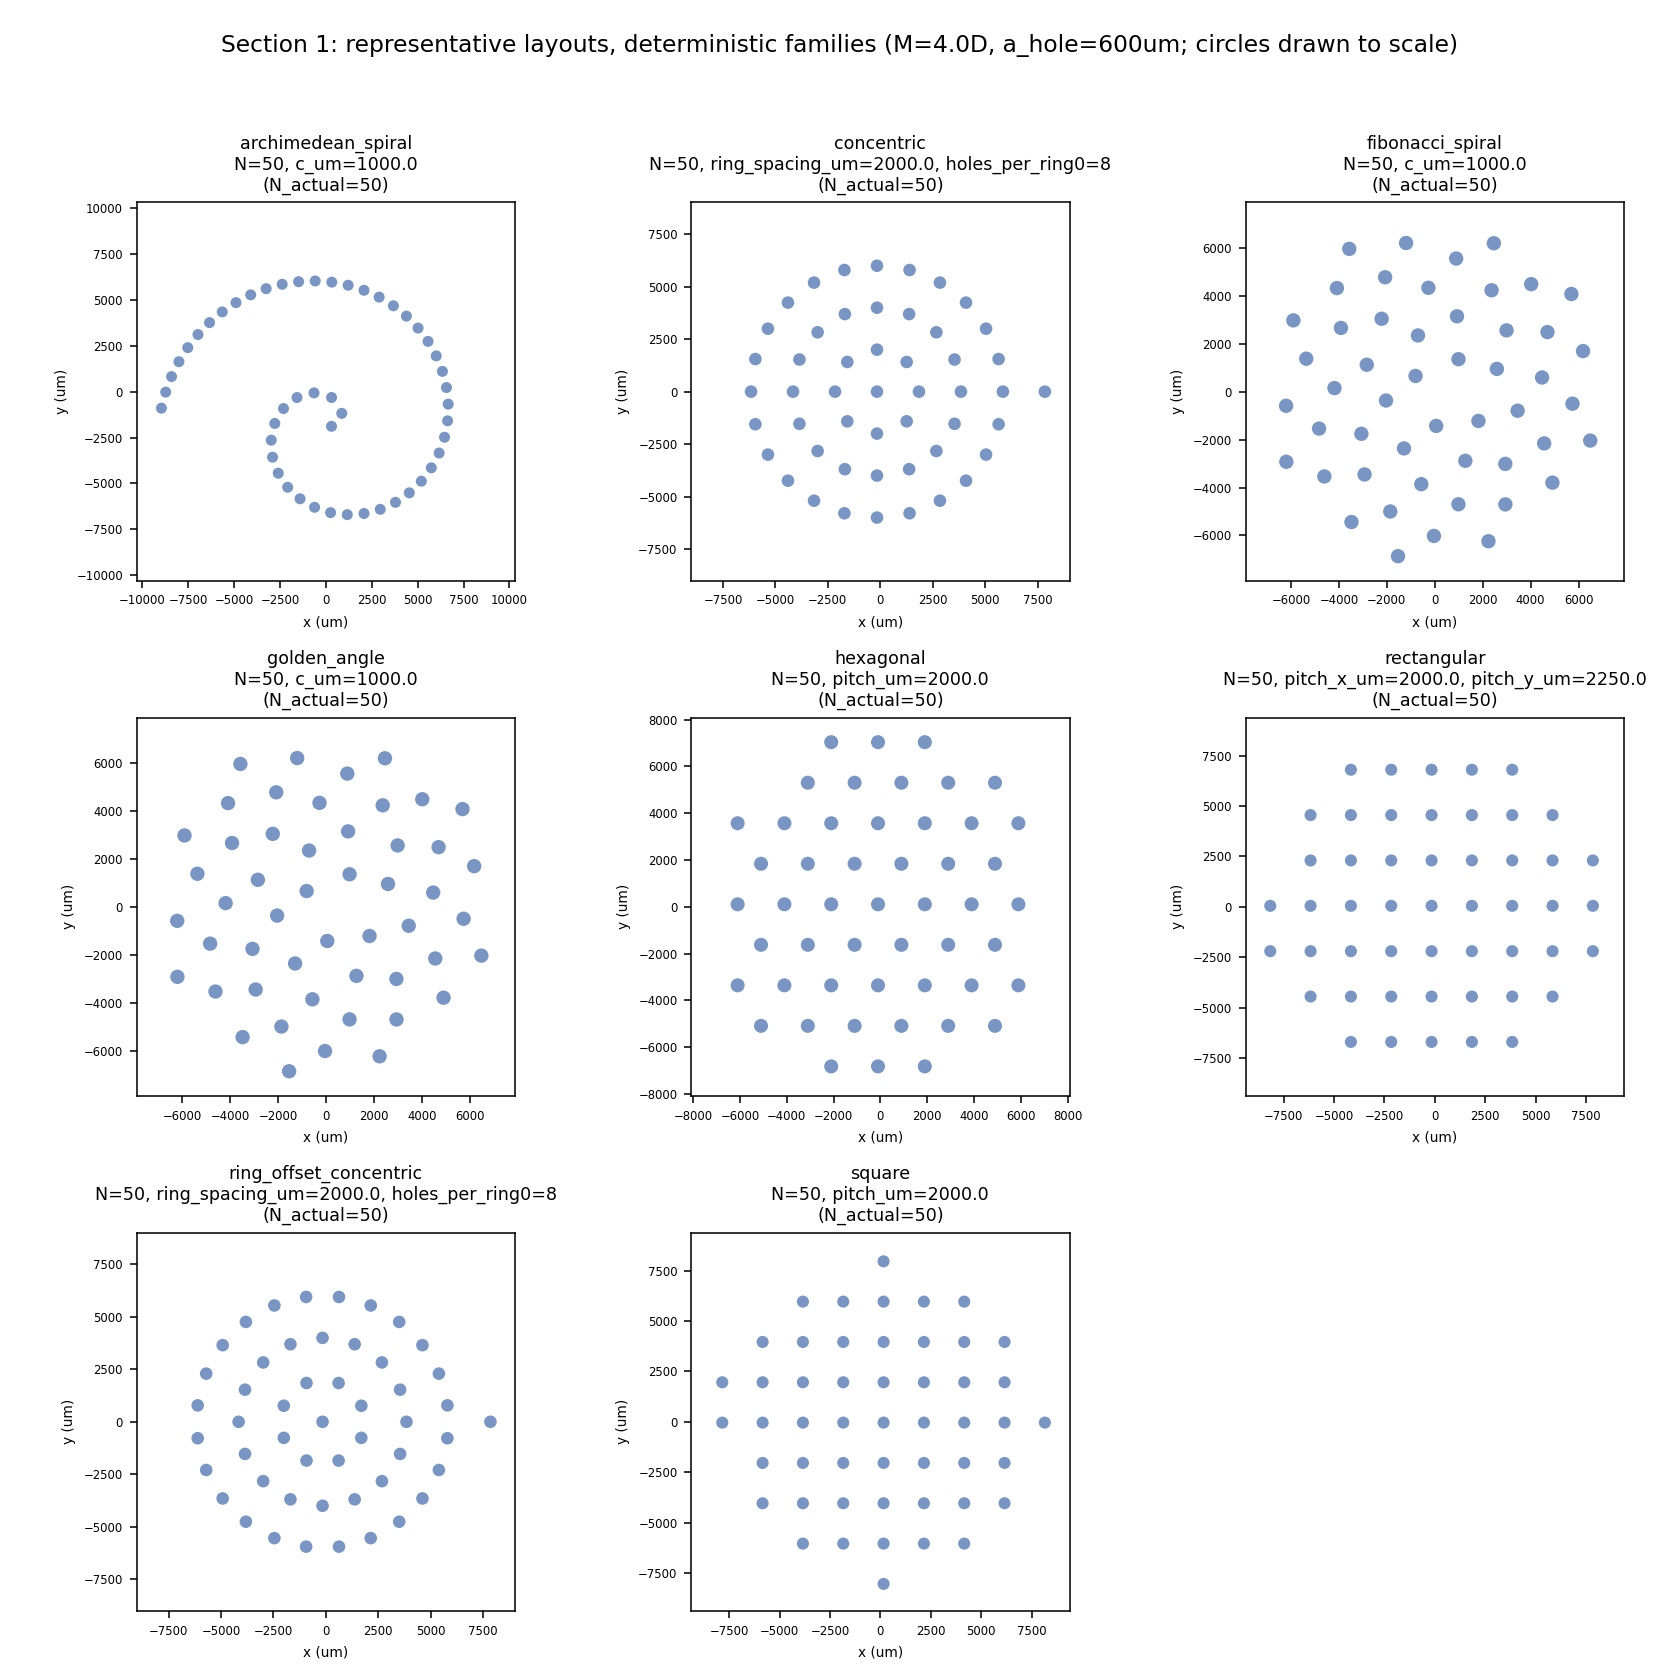
\includegraphics[width=0.95\textwidth]{figs_exploration/section1_deterministic_catalog.png}
\caption{Representative layout, all 8 deterministic families, at their own mid-range
tested $(N, \text{spacing})$.}
\end{figure}
\clearpage
\begin{figure}[h!]
\centering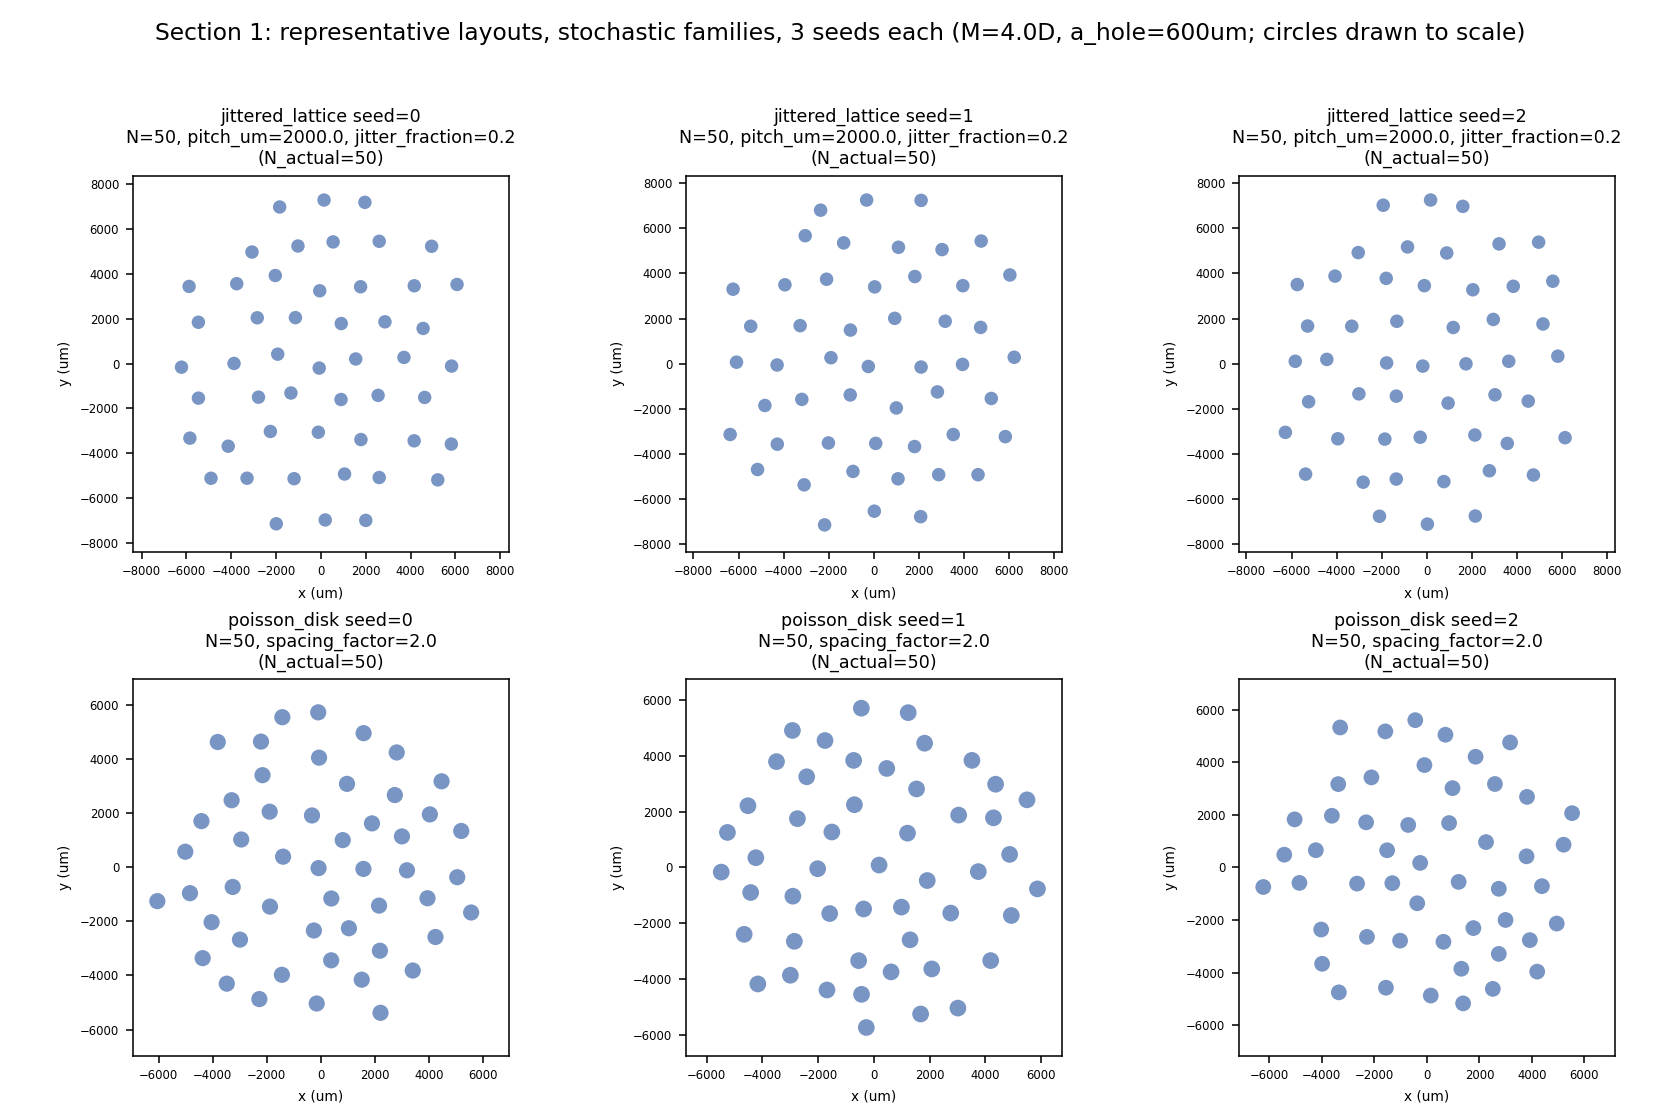
\includegraphics[width=0.95\textwidth]{figs_exploration/section1_stochastic_catalog.png}
\caption{Representative layout, both stochastic families, 3 seeds each (same
$N$/spacing point, seed 0/1/2) -- the visible difference between panels in a row is
seed-driven layout variation at fixed parameters.}
\end{figure}
\clearpage

%======================================================================
\chapter{Margin Heatmaps}
\label{ch:heatmaps}
%======================================================================
For each family, four items, in this order: (1) a heatmap of
\texttt{worst\_case\_ghost\_margin} and \texttt{worst\_case\_vignetting\_margin} over
$(N, \text{primary spacing parameter})$, one small panel per tested $M$ (including
\texttt{global}) -- \textbf{every cell is now annotated with its own exact numeric
value} (or \texttt{inf}), not color alone; (2) a sign-agreement map over the same axes,
coloring each cell by whether the two margins' \emph{signs} agree (both positive, both
negative) or disagree, per $M$; (3) a line-plot view of the same data (margin vs.\ $N$,
one line per primary spacing value, faceted by $M$) as a complementary graphical
representation for reading trends across $N$ directly, which a color grid can obscure;
(4) a raw number list -- one row per tested $(N, \text{primary spacing}, M)$ point,
listing the exact \texttt{worst\_case\_ghost\_margin}/\texttt{worst\_case\_vignetting\_margin}
values with no clipping or color encoding, for readers who want the literal numbers
behind items (1)--(3). Where a family has a secondary spacing parameter (e.g.\
\texttt{holes\_per\_ring0}, \texttt{jitter\_fraction}), it is held fixed at its own
median tested value -- stated in each heatmap's own caption/subtitle -- so every
heatmap's two axes are exactly $(N, \text{primary spacing})$, nothing folded in
silently. For the two stochastic families, every cell (heatmap, line plot, and raw
table alike) is the seed-aggregated worst-case value computed directly from
\texttt{sweep\_results.csv} over \emph{all} tested seeds at that point -- not only the
seeds that happened to end up in \texttt{family\_ranking.csv}'s safe-only subset, which
would silently leave gaps at every unsafe point (a real gap in an earlier draft of this
chapter, fixed by computing all four items from one shared grid-builder function
that reads the full sweep, both here and in Chapter~\ref{ch:seedvariance}). Per-seed
\emph{distributional} detail (the spread across individual seeds, not just their
worst-case) remains Chapter~\ref{ch:seedvariance}'s job.

\textbf{Color/display convention, stated once}: heatmap color is clipped to $[-5, 5]$;
a cell with $+\infty$ margin (zero active hole pairs under the pupil -- a structural,
not narrowly-numerical, safe result) is shown at the clipped color maximum but its
printed cell text always reads \texttt{inf}, and the raw number list always reports the
literal value -- clipping is a display-only convention for the color scale, never
applied to any number actually printed or listed.

\section{archimedean\_spiral}
\begin{figure}[h!]
\centering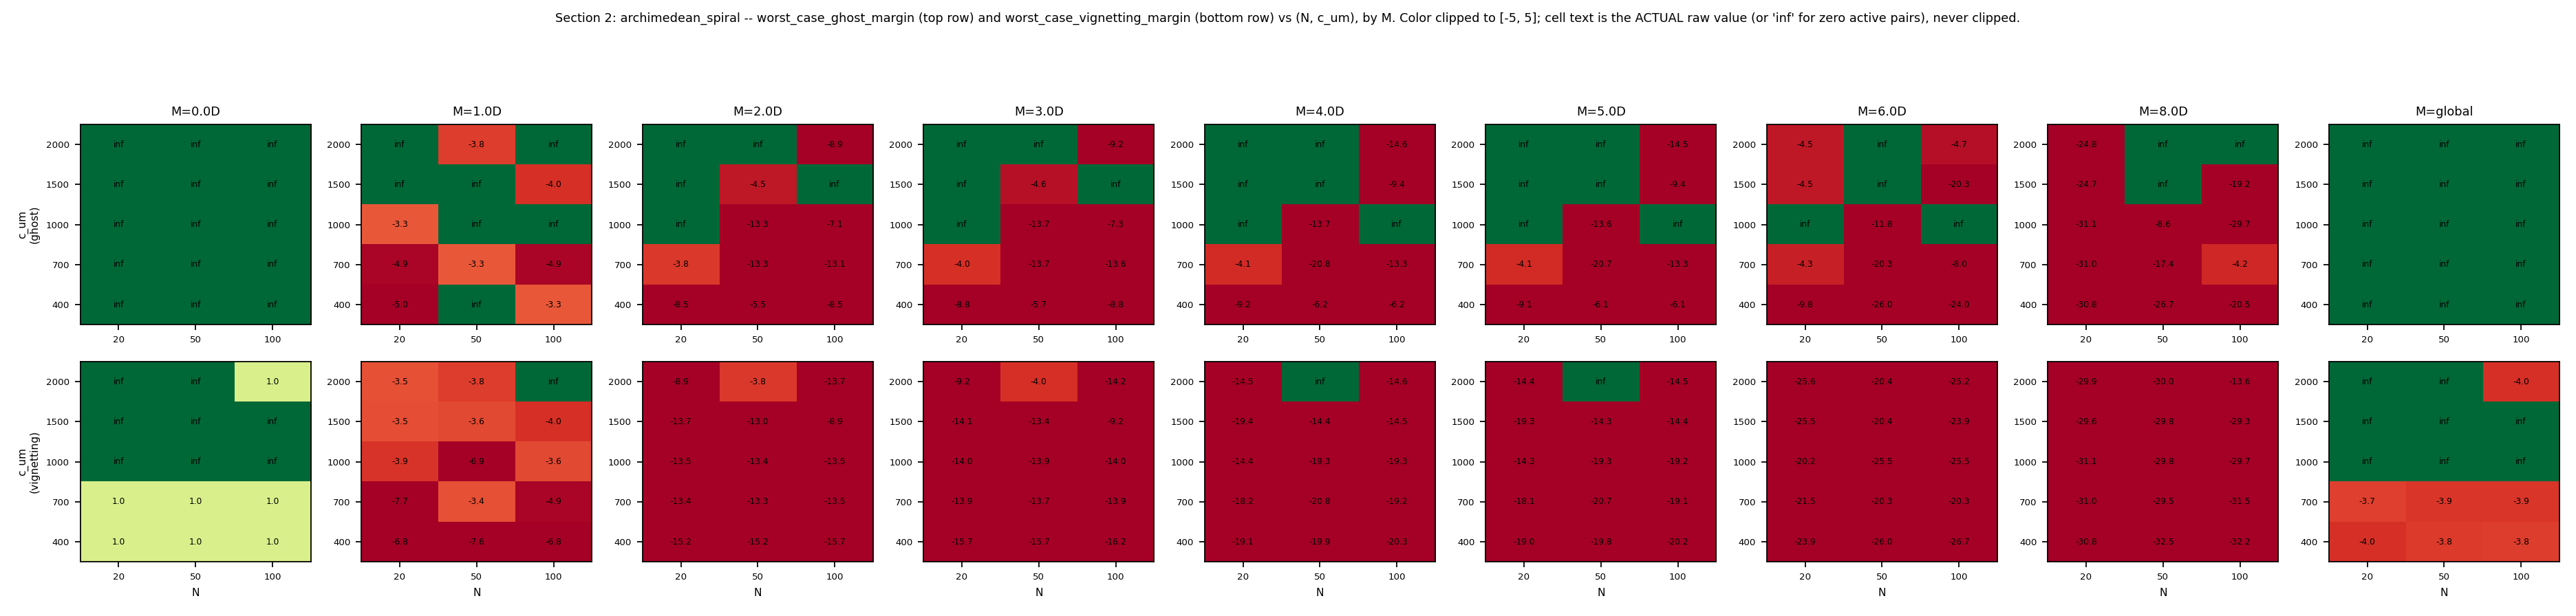
\includegraphics[width=\textwidth]{figs_exploration/section2_heatmap_archimedean_spiral.png}
\caption{archimedean\_spiral: worst\_case\_ghost\_margin (top row) and worst\_case\_vignetting\_margin (bottom row) vs.\ $(N, \text{c\_um})$, by $M$. axes: $N \in \{20,50,100\}$.}
\end{figure}
\begin{figure}[h!]
\centering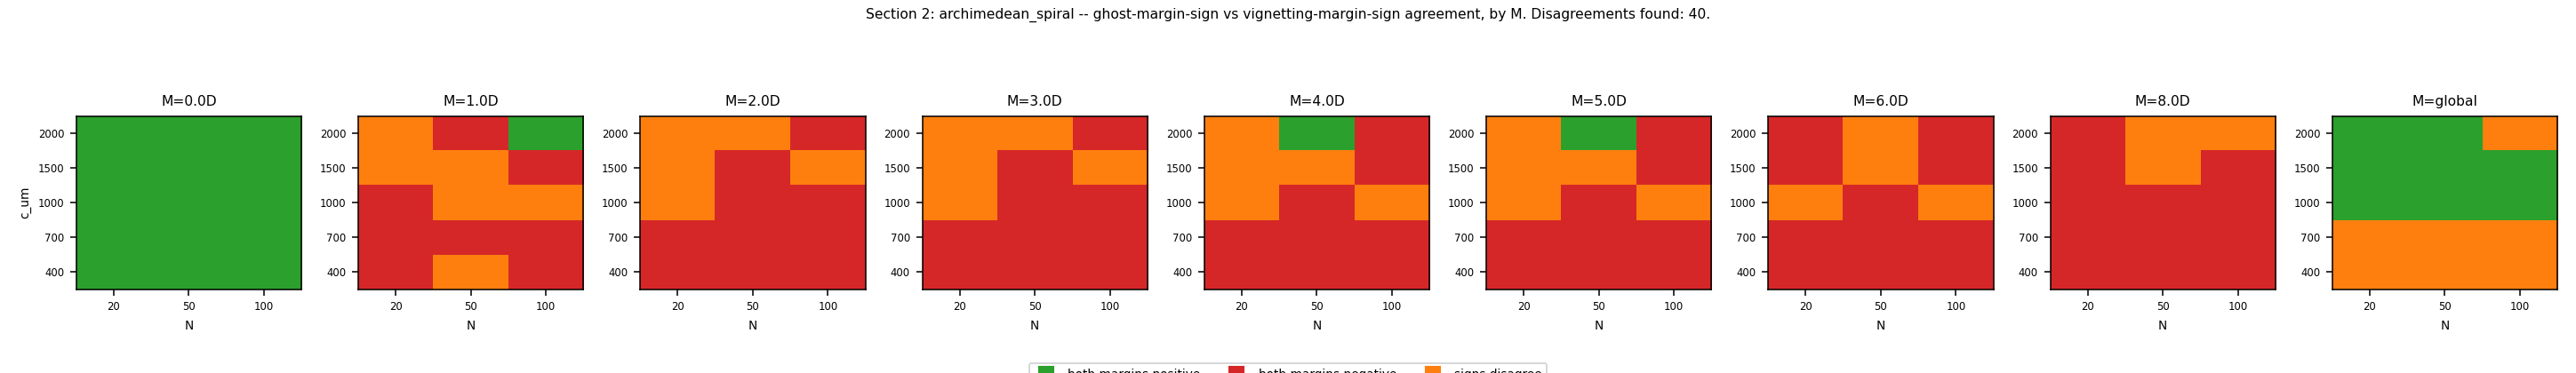
\includegraphics[width=\textwidth]{figs_exploration/section2_signagreement_archimedean_spiral.png}
\caption{archimedean\_spiral: ghost-margin-sign vs.\ vignetting-margin-sign agreement, by $M$ (see the figure's own title for the exact disagreement count).}
\end{figure}
\clearpage
\begin{figure}[h!]
\centering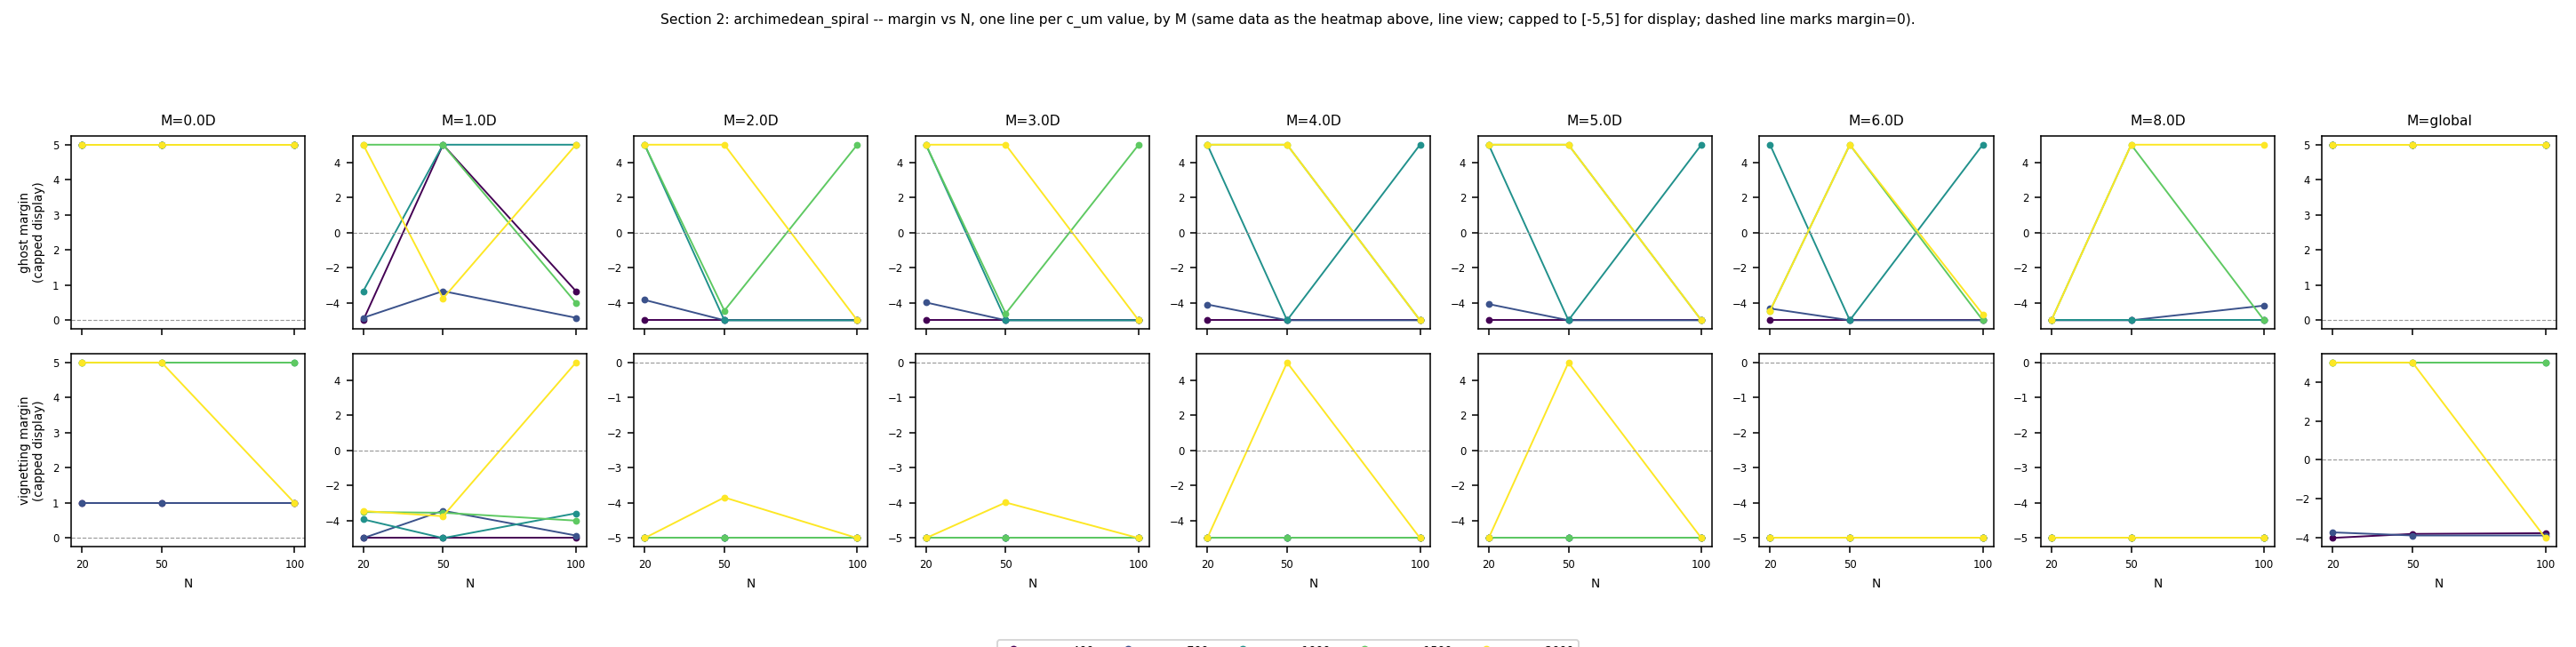
\includegraphics[width=\textwidth]{figs_exploration/section2_lineplot_archimedean_spiral.png}
\caption{archimedean\_spiral: same margin data as the heatmap above, shown as line plots (margin vs.\ $N$, one line per c\_um value) -- a complementary graphical view for reading trends across $N$ directly.}
\end{figure}
\clearpage
\subsection*{archimedean\_spiral: raw number list}
\begin{longtable}{rrrrr}
\caption{archimedean\_spiral: raw worst\_case\_ghost\_margin and worst\_case\_vignetting\_margin values behind the heatmap and line plot above -- one row per tested $(N, c\_um, M)$ point. `inf' = zero active hole pairs under the pupil at that point (structurally safe, undisplayable on a linear scale).} \\
\toprule
N & c\_um & M & ghost\_margin & vignetting\_margin \\
\midrule
\endfirsthead
\toprule
N & c\_um & M & ghost\_margin & vignetting\_margin \\
\midrule
\endhead
\midrule
\multicolumn{5}{r}{\itshape continued on next page} \\
\endfoot
\bottomrule
\endlastfoot
20 & 400 & 0D & inf & 1.000 \\
20 & 400 & 1D & -4.996 & -6.762 \\
20 & 400 & 2D & -8.487 & -15.237 \\
20 & 400 & 3D & -8.768 & -15.717 \\
20 & 400 & 4D & -9.186 & -19.128 \\
20 & 400 & 5D & -9.143 & -19.042 \\
20 & 400 & 6D & -9.800 & -23.865 \\
20 & 400 & 8D & -30.798 & -30.798 \\
20 & 400 & global & inf & -4.013 \\
50 & 400 & 0D & inf & 1.000 \\
50 & 400 & 1D & inf & -7.624 \\
50 & 400 & 2D & -5.465 & -15.237 \\
50 & 400 & 3D & -5.656 & -15.717 \\
50 & 400 & 4D & -6.173 & -19.874 \\
50 & 400 & 5D & -6.142 & -19.785 \\
50 & 400 & 6D & -25.994 & -26.044 \\
50 & 400 & 8D & -26.702 & -32.483 \\
50 & 400 & global & inf & -3.808 \\
100 & 400 & 0D & inf & 1.000 \\
100 & 400 & 1D & -3.337 & -6.762 \\
100 & 400 & 2D & -8.487 & -15.747 \\
100 & 400 & 3D & -8.768 & -16.243 \\
100 & 400 & 4D & -6.173 & -20.254 \\
100 & 400 & 5D & -6.142 & -20.164 \\
100 & 400 & 6D & -24.034 & -26.733 \\
100 & 400 & 8D & -20.535 & -32.226 \\
100 & 400 & global & inf & -3.770 \\
20 & 700 & 0D & inf & 1.000 \\
20 & 700 & 1D & -4.854 & -7.683 \\
20 & 700 & 2D & -3.842 & -13.442 \\
20 & 700 & 3D & -3.986 & -13.869 \\
20 & 700 & 4D & -4.101 & -18.192 \\
20 & 700 & 5D & -4.079 & -18.111 \\
20 & 700 & 6D & -4.331 & -21.487 \\
20 & 700 & 8D & -31.017 & -31.017 \\
20 & 700 & global & inf & -3.729 \\
50 & 700 & 0D & inf & 1.000 \\
50 & 700 & 1D & -3.337 & -3.441 \\
50 & 700 & 2D & -13.291 & -13.291 \\
50 & 700 & 3D & -13.714 & -13.714 \\
50 & 700 & 4D & -20.806 & -20.806 \\
50 & 700 & 5D & -20.713 & -20.713 \\
50 & 700 & 6D & -20.265 & -20.265 \\
50 & 700 & 8D & -17.356 & -29.462 \\
50 & 700 & global & inf & -3.888 \\
100 & 700 & 0D & inf & 1.000 \\
100 & 700 & 1D & -4.854 & -4.854 \\
100 & 700 & 2D & -13.145 & -13.496 \\
100 & 700 & 3D & -13.563 & -13.925 \\
100 & 700 & 4D & -13.324 & -19.154 \\
100 & 700 & 5D & -13.263 & -19.069 \\
100 & 700 & 6D & -7.969 & -20.265 \\
100 & 700 & 8D & -4.164 & -31.532 \\
100 & 700 & global & inf & -3.888 \\
20 & 1000 & 0D & inf & inf \\
20 & 1000 & 1D & -3.337 & -3.934 \\
20 & 1000 & 2D & inf & -13.547 \\
20 & 1000 & 3D & inf & -13.977 \\
20 & 1000 & 4D & inf & -14.393 \\
20 & 1000 & 5D & inf & -14.327 \\
20 & 1000 & 6D & inf & -20.212 \\
20 & 1000 & 8D & -31.099 & -31.099 \\
20 & 1000 & global & inf & inf \\
50 & 1000 & 0D & inf & inf \\
50 & 1000 & 1D & inf & -6.857 \\
50 & 1000 & 2D & -13.285 & -13.430 \\
50 & 1000 & 3D & -13.708 & -13.857 \\
50 & 1000 & 4D & -13.661 & -19.347 \\
50 & 1000 & 5D & -13.599 & -19.260 \\
50 & 1000 & 6D & -11.770 & -25.505 \\
50 & 1000 & 8D & -8.593 & -29.771 \\
50 & 1000 & global & inf & inf \\
100 & 1000 & 0D & inf & inf \\
100 & 1000 & 1D & inf & -3.588 \\
100 & 1000 & 2D & -7.060 & -13.546 \\
100 & 1000 & 3D & -7.298 & -13.976 \\
100 & 1000 & 4D & inf & -19.332 \\
100 & 1000 & 5D & inf & -19.246 \\
100 & 1000 & 6D & inf & -25.467 \\
100 & 1000 & 8D & -29.705 & -29.705 \\
100 & 1000 & global & inf & inf \\
20 & 1500 & 0D & inf & inf \\
20 & 1500 & 1D & inf & -3.515 \\
20 & 1500 & 2D & inf & -13.655 \\
20 & 1500 & 3D & inf & -14.088 \\
20 & 1500 & 4D & inf & -19.411 \\
20 & 1500 & 5D & inf & -19.324 \\
20 & 1500 & 6D & -4.460 & -25.456 \\
20 & 1500 & 8D & -24.713 & -29.565 \\
20 & 1500 & global & inf & inf \\
50 & 1500 & 0D & inf & inf \\
50 & 1500 & 1D & inf & -3.556 \\
50 & 1500 & 2D & -4.455 & -13.024 \\
50 & 1500 & 3D & -4.616 & -13.439 \\
50 & 1500 & 4D & inf & -14.362 \\
50 & 1500 & 5D & inf & -14.297 \\
50 & 1500 & 6D & inf & -20.367 \\
50 & 1500 & 8D & inf & -29.813 \\
50 & 1500 & global & inf & inf \\
100 & 1500 & 0D & inf & inf \\
100 & 1500 & 1D & -4.005 & -4.005 \\
100 & 1500 & 2D & inf & -8.862 \\
100 & 1500 & 3D & inf & -9.154 \\
100 & 1500 & 4D & -9.426 & -14.486 \\
100 & 1500 & 5D & -9.382 & -14.420 \\
100 & 1500 & 6D & -20.254 & -23.931 \\
100 & 1500 & 8D & -19.189 & -29.253 \\
100 & 1500 & global & inf & inf \\
20 & 2000 & 0D & inf & inf \\
20 & 2000 & 1D & inf & -3.457 \\
20 & 2000 & 2D & inf & -8.864 \\
20 & 2000 & 3D & inf & -9.155 \\
20 & 2000 & 4D & inf & -14.502 \\
20 & 2000 & 5D & inf & -14.436 \\
20 & 2000 & 6D & -4.462 & -25.642 \\
20 & 2000 & 8D & -24.835 & -29.860 \\
20 & 2000 & global & inf & inf \\
50 & 2000 & 0D & inf & inf \\
50 & 2000 & 1D & -3.753 & -3.753 \\
50 & 2000 & 2D & inf & -3.842 \\
50 & 2000 & 3D & inf & -3.986 \\
50 & 2000 & 4D & inf & inf \\
50 & 2000 & 5D & inf & inf \\
50 & 2000 & 6D & inf & -20.434 \\
50 & 2000 & 8D & inf & -29.960 \\
50 & 2000 & global & inf & inf \\
100 & 2000 & 0D & inf & 1.000 \\
100 & 2000 & 1D & inf & inf \\
100 & 2000 & 2D & -8.927 & -13.727 \\
100 & 2000 & 3D & -9.220 & -14.162 \\
100 & 2000 & 4D & -14.604 & -14.604 \\
100 & 2000 & 5D & -14.538 & -14.538 \\
100 & 2000 & 6D & -4.660 & -25.192 \\
100 & 2000 & 8D & inf & -13.564 \\
100 & 2000 & global & inf & -4.023 \\
\end{longtable}

\clearpage

\section{concentric}
\begin{figure}[h!]
\centering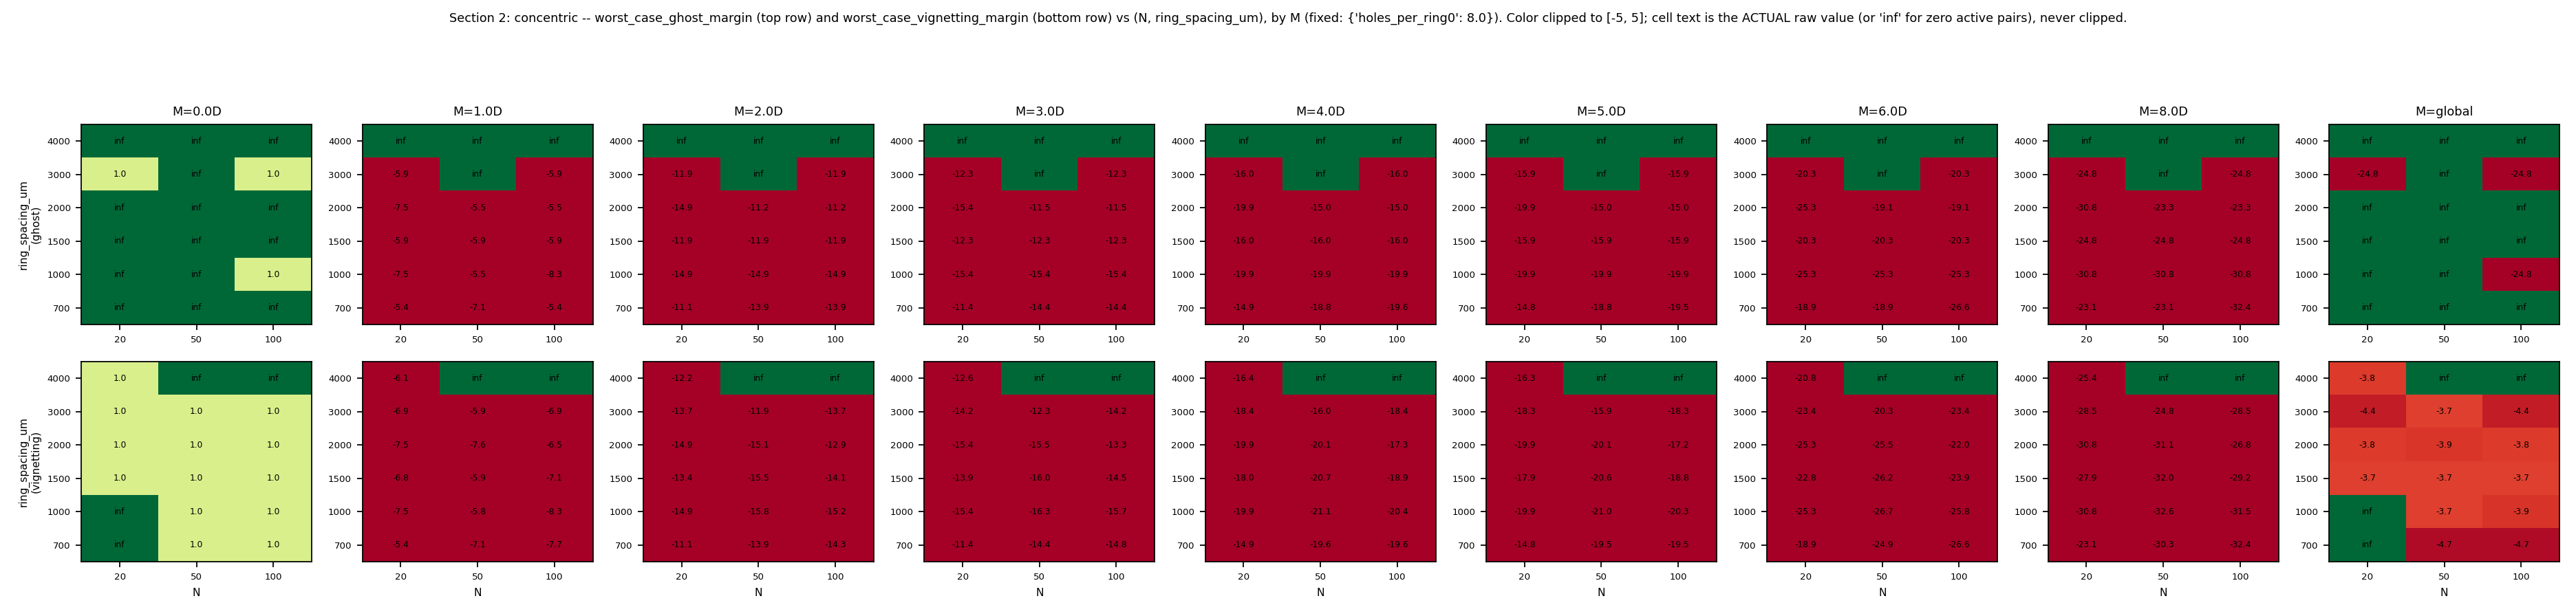
\includegraphics[width=\textwidth]{figs_exploration/section2_heatmap_concentric.png}
\caption{concentric: worst\_case\_ghost\_margin (top row) and worst\_case\_vignetting\_margin (bottom row) vs.\ $(N, \text{ring\_spacing\_um})$, by $M$. holes\_per\_ring0=8.0 held fixed at its own median tested value; axes: $N \in \{20,50,100\}$.}
\end{figure}
\begin{figure}[h!]
\centering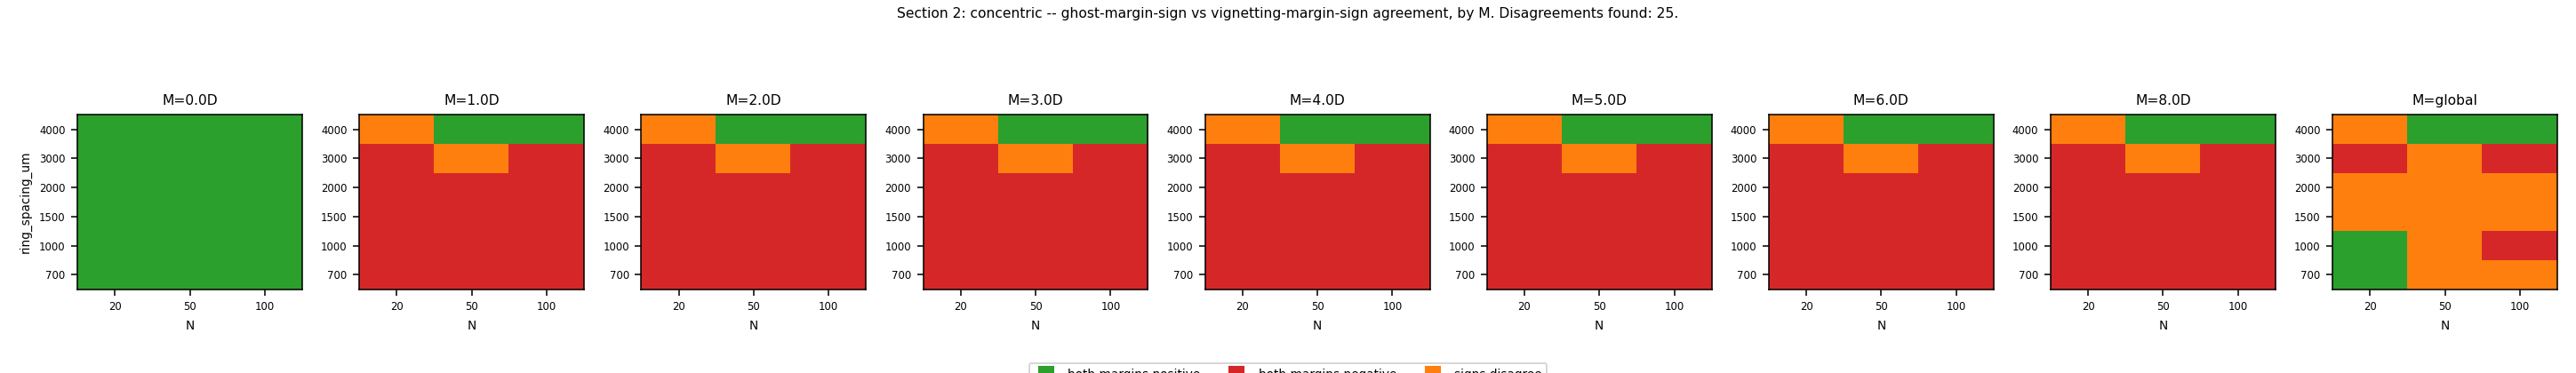
\includegraphics[width=\textwidth]{figs_exploration/section2_signagreement_concentric.png}
\caption{concentric: ghost-margin-sign vs.\ vignetting-margin-sign agreement, by $M$ (see the figure's own title for the exact disagreement count).}
\end{figure}
\clearpage
\begin{figure}[h!]
\centering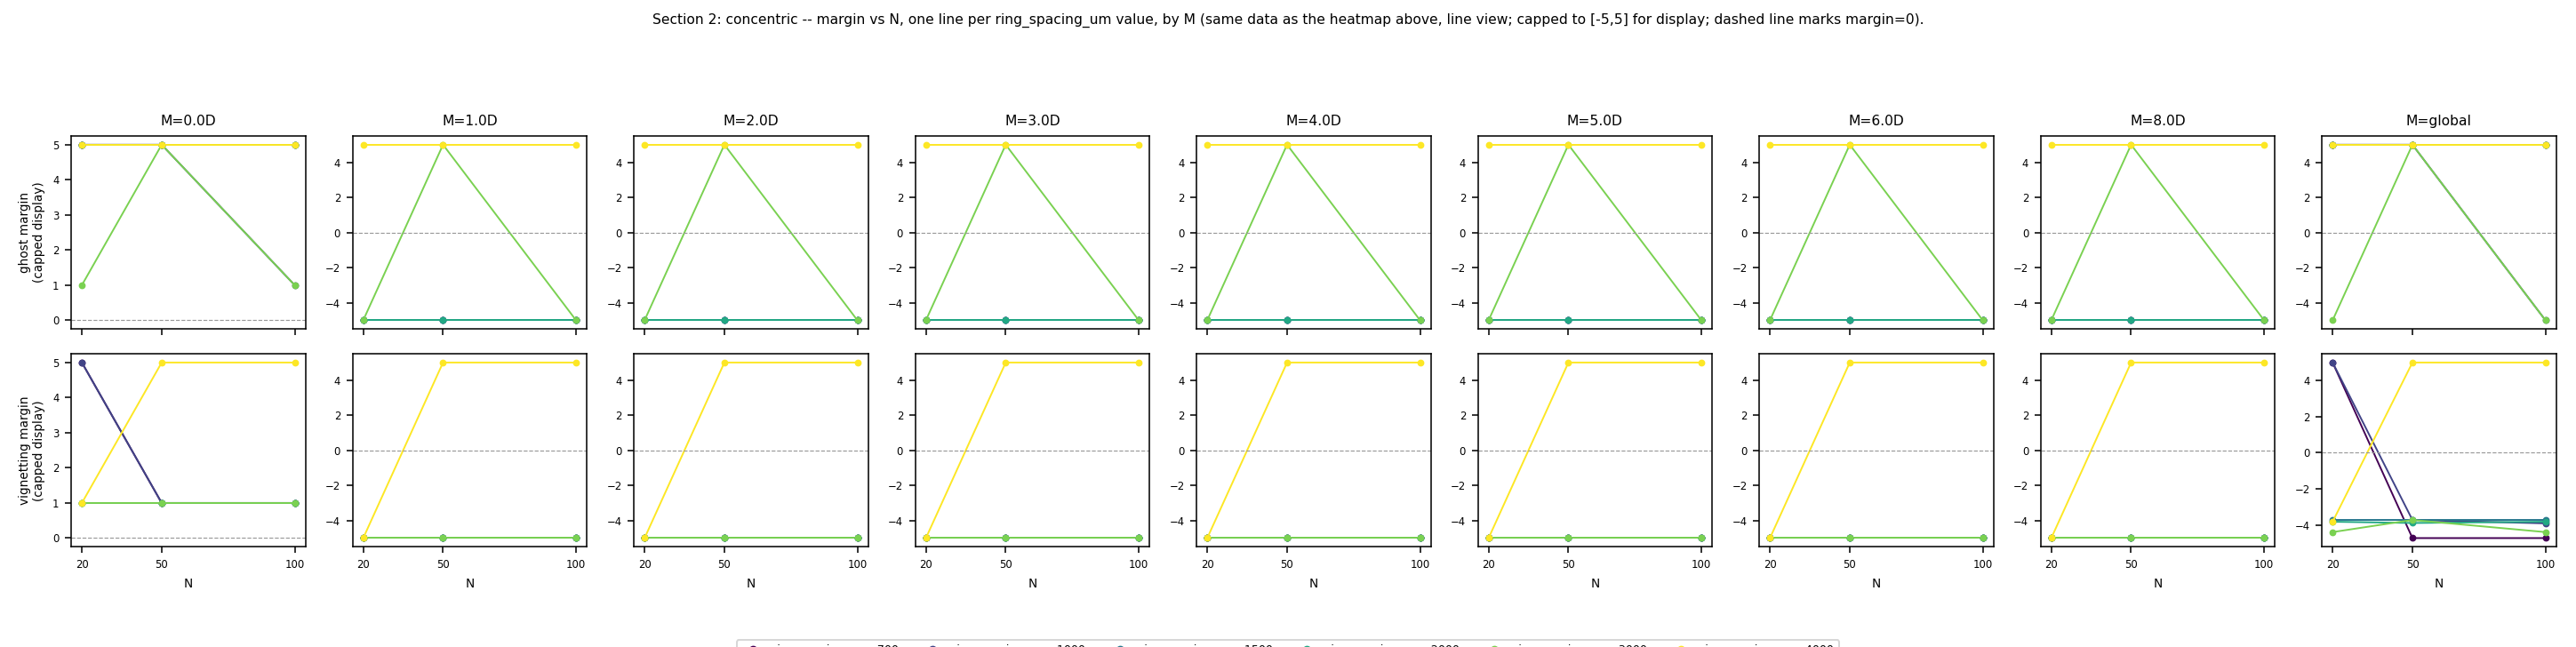
\includegraphics[width=\textwidth]{figs_exploration/section2_lineplot_concentric.png}
\caption{concentric: same margin data as the heatmap above, shown as line plots (margin vs.\ $N$, one line per ring\_spacing\_um value) -- a complementary graphical view for reading trends across $N$ directly.}
\end{figure}
\clearpage
\subsection*{concentric: raw number list}
\begin{longtable}{rrrrr}
\caption{concentric: raw worst\_case\_ghost\_margin and worst\_case\_vignetting\_margin values behind the heatmap and line plot above -- one row per tested $(N, ring\_spacing\_um, M)$ point. `inf' = zero active hole pairs under the pupil at that point (structurally safe, undisplayable on a linear scale).} \\
\toprule
N & ring\_spacing\_um & M & ghost\_margin & vignetting\_margin \\
\midrule
\endfirsthead
\toprule
N & ring\_spacing\_um & M & ghost\_margin & vignetting\_margin \\
\midrule
\endhead
\midrule
\multicolumn{5}{r}{\itshape continued on next page} \\
\endfoot
\bottomrule
\endlastfoot
20 & 700 & 0D & inf & inf \\
20 & 700 & 1D & -5.352 & -5.352 \\
20 & 700 & 2D & -11.052 & -11.052 \\
20 & 700 & 3D & -11.408 & -11.408 \\
20 & 700 & 4D & -14.870 & -14.870 \\
20 & 700 & 5D & -14.802 & -14.802 \\
20 & 700 & 6D & -18.904 & -18.904 \\
20 & 700 & 8D & -23.100 & -23.100 \\
20 & 700 & global & inf & inf \\
50 & 700 & 0D & inf & 1.000 \\
50 & 700 & 1D & -7.096 & -7.096 \\
50 & 700 & 2D & -13.942 & -13.942 \\
50 & 700 & 3D & -14.383 & -14.383 \\
50 & 700 & 4D & -18.837 & -19.615 \\
50 & 700 & 5D & -18.753 & -19.528 \\
50 & 700 & 6D & -18.904 & -24.856 \\
50 & 700 & 8D & -23.100 & -30.307 \\
50 & 700 & global & inf & -4.733 \\
100 & 700 & 0D & inf & 1.000 \\
100 & 700 & 1D & -5.352 & -7.703 \\
100 & 700 & 2D & -13.942 & -14.326 \\
100 & 700 & 3D & -14.383 & -14.779 \\
100 & 700 & 4D & -19.615 & -19.615 \\
100 & 700 & 5D & -19.528 & -19.528 \\
100 & 700 & 6D & -26.583 & -26.583 \\
100 & 700 & 8D & -32.399 & -32.399 \\
100 & 700 & global & inf & -4.733 \\
20 & 1000 & 0D & inf & inf \\
20 & 1000 & 1D & -7.548 & -7.548 \\
20 & 1000 & 2D & -14.907 & -14.907 \\
20 & 1000 & 3D & -15.377 & -15.377 \\
20 & 1000 & 4D & -19.945 & -19.945 \\
20 & 1000 & 5D & -19.857 & -19.857 \\
20 & 1000 & 6D & -25.270 & -25.270 \\
20 & 1000 & 8D & -30.808 & -30.808 \\
20 & 1000 & global & inf & inf \\
50 & 1000 & 0D & inf & 1.000 \\
50 & 1000 & 1D & -5.542 & -5.817 \\
50 & 1000 & 2D & -14.907 & -15.779 \\
50 & 1000 & 3D & -15.377 & -16.275 \\
50 & 1000 & 4D & -19.945 & -21.094 \\
50 & 1000 & 5D & -19.857 & -21.001 \\
50 & 1000 & 6D & -25.270 & -26.711 \\
50 & 1000 & 8D & -30.808 & -32.553 \\
50 & 1000 & global & inf & -3.729 \\
100 & 1000 & 0D & 1.000 & 1.000 \\
100 & 1000 & 1D & -8.252 & -8.252 \\
100 & 1000 & 2D & -14.907 & -15.244 \\
100 & 1000 & 3D & -15.377 & -15.725 \\
100 & 1000 & 4D & -19.945 & -20.390 \\
100 & 1000 & 5D & -19.857 & -20.299 \\
100 & 1000 & 6D & -25.270 & -25.827 \\
100 & 1000 & 8D & -30.808 & -31.483 \\
100 & 1000 & global & -24.822 & -3.916 \\
20 & 1500 & 0D & inf & 1.000 \\
20 & 1500 & 1D & -5.939 & -6.758 \\
20 & 1500 & 2D & -11.913 & -13.437 \\
20 & 1500 & 3D & -12.295 & -13.864 \\
20 & 1500 & 4D & -16.003 & -18.010 \\
20 & 1500 & 5D & -15.931 & -17.930 \\
20 & 1500 & 6D & -20.326 & -22.843 \\
20 & 1500 & 8D & -24.822 & -27.870 \\
20 & 1500 & global & inf & -3.729 \\
50 & 1500 & 0D & inf & 1.000 \\
50 & 1500 & 1D & -5.939 & -5.939 \\
50 & 1500 & 2D & -11.913 & -15.500 \\
50 & 1500 & 3D & -12.295 & -15.988 \\
50 & 1500 & 4D & -16.003 & -20.726 \\
50 & 1500 & 5D & -15.931 & -20.634 \\
50 & 1500 & 6D & -20.326 & -26.249 \\
50 & 1500 & 8D & -24.822 & -31.994 \\
50 & 1500 & global & inf & -3.729 \\
100 & 1500 & 0D & inf & 1.000 \\
100 & 1500 & 1D & -5.939 & -7.113 \\
100 & 1500 & 2D & -11.913 & -14.098 \\
100 & 1500 & 3D & -12.295 & -14.545 \\
100 & 1500 & 4D & -16.003 & -18.881 \\
100 & 1500 & 5D & -15.931 & -18.796 \\
100 & 1500 & 6D & -20.326 & -23.934 \\
100 & 1500 & 8D & -24.822 & -29.191 \\
100 & 1500 & global & inf & -3.729 \\
20 & 2000 & 0D & inf & 1.000 \\
20 & 2000 & 1D & -7.548 & -7.548 \\
20 & 2000 & 2D & -14.907 & -14.907 \\
20 & 2000 & 3D & -15.377 & -15.377 \\
20 & 2000 & 4D & -19.945 & -19.945 \\
20 & 2000 & 5D & -19.857 & -19.857 \\
20 & 2000 & 6D & -25.270 & -25.270 \\
20 & 2000 & 8D & -30.808 & -30.808 \\
20 & 2000 & global & inf & -3.825 \\
50 & 2000 & 0D & inf & 1.000 \\
50 & 2000 & 1D & -5.542 & -7.630 \\
50 & 2000 & 2D & -11.175 & -15.059 \\
50 & 2000 & 3D & -11.534 & -15.534 \\
50 & 2000 & 4D & -15.031 & -20.145 \\
50 & 2000 & 5D & -14.963 & -20.056 \\
50 & 2000 & 6D & -19.106 & -25.521 \\
50 & 2000 & 8D & -23.345 & -31.112 \\
50 & 2000 & global & inf & -3.895 \\
100 & 2000 & 0D & inf & 1.000 \\
100 & 2000 & 1D & -5.542 & -6.470 \\
100 & 2000 & 2D & -11.175 & -12.902 \\
100 & 2000 & 3D & -11.534 & -13.313 \\
100 & 2000 & 4D & -15.031 & -17.305 \\
100 & 2000 & 5D & -14.963 & -17.227 \\
100 & 2000 & 6D & -19.106 & -21.958 \\
100 & 2000 & 8D & -23.345 & -26.799 \\
100 & 2000 & global & inf & -3.825 \\
20 & 3000 & 0D & 1.000 & 1.000 \\
20 & 3000 & 1D & -5.939 & -6.926 \\
20 & 3000 & 2D & -11.913 & -13.748 \\
20 & 3000 & 3D & -12.295 & -14.185 \\
20 & 3000 & 4D & -16.003 & -18.420 \\
20 & 3000 & 5D & -15.931 & -18.338 \\
20 & 3000 & 6D & -20.326 & -23.357 \\
20 & 3000 & 8D & -24.822 & -28.492 \\
20 & 3000 & global & -24.822 & -4.401 \\
50 & 3000 & 0D & inf & 1.000 \\
50 & 3000 & 1D & inf & -5.939 \\
50 & 3000 & 2D & inf & -11.913 \\
50 & 3000 & 3D & inf & -12.295 \\
50 & 3000 & 4D & inf & -16.003 \\
50 & 3000 & 5D & inf & -15.931 \\
50 & 3000 & 6D & inf & -20.326 \\
50 & 3000 & 8D & inf & -24.822 \\
50 & 3000 & global & inf & -3.729 \\
100 & 3000 & 0D & 1.000 & 1.000 \\
100 & 3000 & 1D & -5.939 & -6.926 \\
100 & 3000 & 2D & -11.913 & -13.748 \\
100 & 3000 & 3D & -12.295 & -14.185 \\
100 & 3000 & 4D & -16.003 & -18.420 \\
100 & 3000 & 5D & -15.931 & -18.338 \\
100 & 3000 & 6D & -20.326 & -23.357 \\
100 & 3000 & 8D & -24.822 & -28.492 \\
100 & 3000 & global & -24.822 & -4.401 \\
20 & 4000 & 0D & inf & 1.000 \\
20 & 4000 & 1D & inf & -6.081 \\
20 & 4000 & 2D & inf & -12.178 \\
20 & 4000 & 3D & inf & -12.567 \\
20 & 4000 & 4D & inf & -16.352 \\
20 & 4000 & 5D & inf & -16.278 \\
20 & 4000 & 6D & inf & -20.763 \\
20 & 4000 & 8D & inf & -25.351 \\
20 & 4000 & global & inf & -3.825 \\
50 & 4000 & 0D & inf & inf \\
50 & 4000 & 1D & inf & inf \\
50 & 4000 & 2D & inf & inf \\
50 & 4000 & 3D & inf & inf \\
50 & 4000 & 4D & inf & inf \\
50 & 4000 & 5D & inf & inf \\
50 & 4000 & 6D & inf & inf \\
50 & 4000 & 8D & inf & inf \\
50 & 4000 & global & inf & inf \\
100 & 4000 & 0D & inf & inf \\
100 & 4000 & 1D & inf & inf \\
100 & 4000 & 2D & inf & inf \\
100 & 4000 & 3D & inf & inf \\
100 & 4000 & 4D & inf & inf \\
100 & 4000 & 5D & inf & inf \\
100 & 4000 & 6D & inf & inf \\
100 & 4000 & 8D & inf & inf \\
100 & 4000 & global & inf & inf \\
\end{longtable}

\clearpage

\section{fibonacci\_spiral}
\begin{figure}[h!]
\centering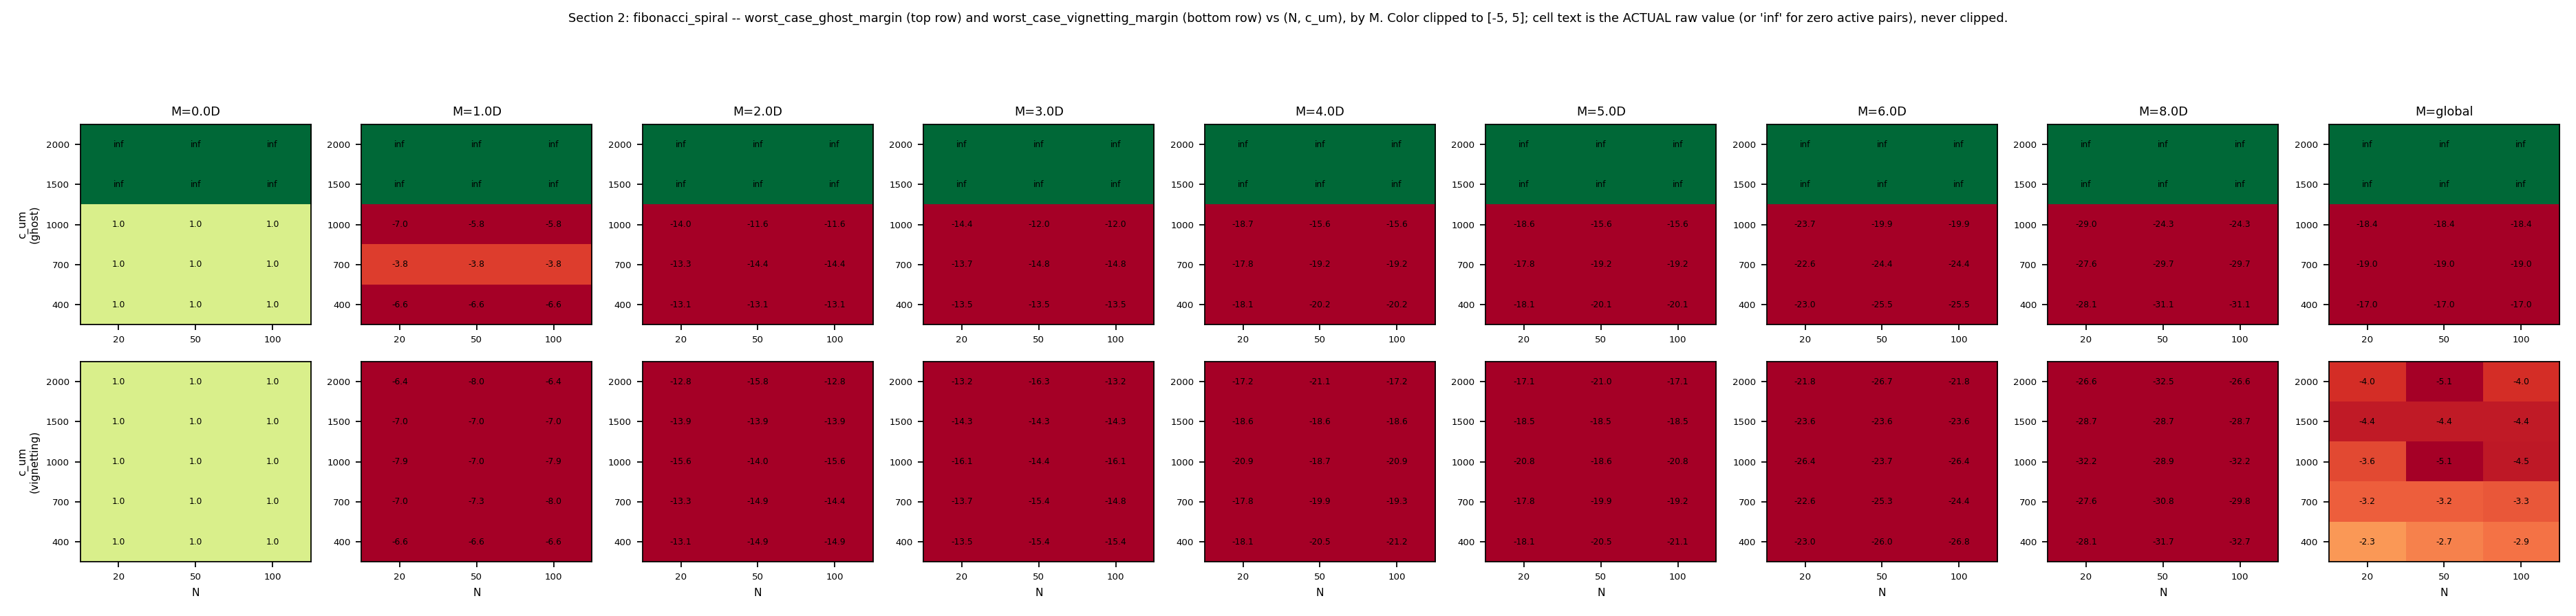
\includegraphics[width=\textwidth]{figs_exploration/section2_heatmap_fibonacci_spiral.png}
\caption{fibonacci\_spiral: worst\_case\_ghost\_margin (top row) and worst\_case\_vignetting\_margin (bottom row) vs.\ $(N, \text{c\_um})$, by $M$. axes: $N \in \{20,50,100\}$.}
\end{figure}
\begin{figure}[h!]
\centering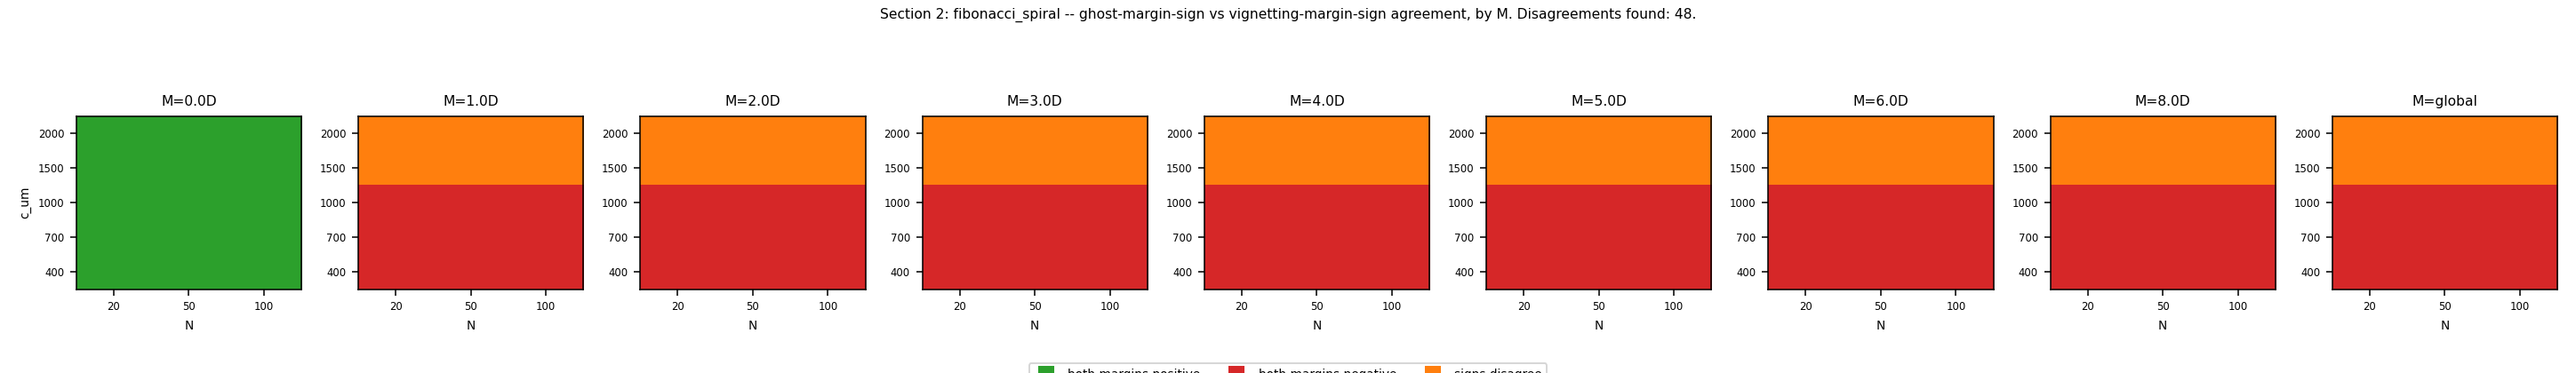
\includegraphics[width=\textwidth]{figs_exploration/section2_signagreement_fibonacci_spiral.png}
\caption{fibonacci\_spiral: ghost-margin-sign vs.\ vignetting-margin-sign agreement, by $M$ (see the figure's own title for the exact disagreement count).}
\end{figure}
\clearpage
\begin{figure}[h!]
\centering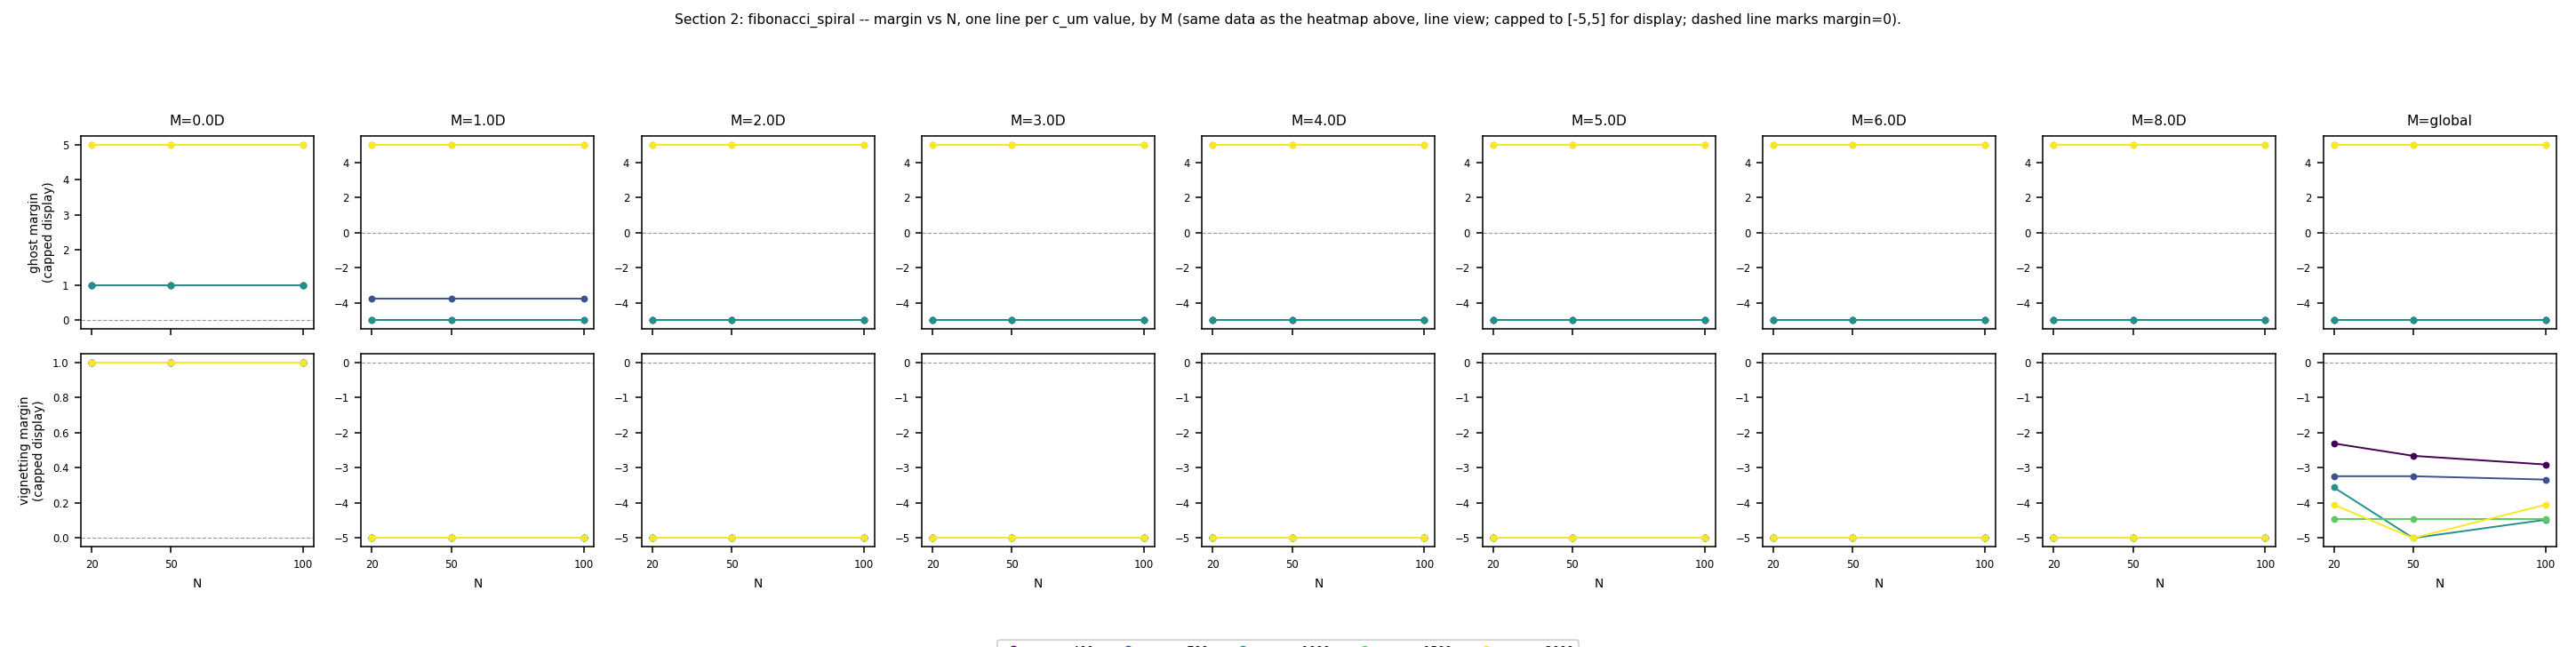
\includegraphics[width=\textwidth]{figs_exploration/section2_lineplot_fibonacci_spiral.png}
\caption{fibonacci\_spiral: same margin data as the heatmap above, shown as line plots (margin vs.\ $N$, one line per c\_um value) -- a complementary graphical view for reading trends across $N$ directly.}
\end{figure}
\clearpage
\subsection*{fibonacci\_spiral: raw number list}
\begin{longtable}{rrrrr}
\caption{fibonacci\_spiral: raw worst\_case\_ghost\_margin and worst\_case\_vignetting\_margin values behind the heatmap and line plot above -- one row per tested $(N, c\_um, M)$ point. `inf' = zero active hole pairs under the pupil at that point (structurally safe, undisplayable on a linear scale).} \\
\toprule
N & c\_um & M & ghost\_margin & vignetting\_margin \\
\midrule
\endfirsthead
\toprule
N & c\_um & M & ghost\_margin & vignetting\_margin \\
\midrule
\endhead
\midrule
\multicolumn{5}{r}{\itshape continued on next page} \\
\endfoot
\bottomrule
\endlastfoot
20 & 400 & 0D & 1.000 & 1.000 \\
20 & 400 & 1D & -6.587 & -6.587 \\
20 & 400 & 2D & -13.119 & -13.119 \\
20 & 400 & 3D & -13.536 & -13.536 \\
20 & 400 & 4D & -18.134 & -18.134 \\
20 & 400 & 5D & -18.053 & -18.053 \\
20 & 400 & 6D & -22.998 & -22.998 \\
20 & 400 & 8D & -28.057 & -28.057 \\
20 & 400 & global & -17.047 & -2.305 \\
50 & 400 & 0D & 1.000 & 1.000 \\
50 & 400 & 1D & -6.587 & -6.587 \\
50 & 400 & 2D & -13.119 & -14.928 \\
50 & 400 & 3D & -13.536 & -15.399 \\
50 & 400 & 4D & -20.164 & -20.542 \\
50 & 400 & 5D & -20.074 & -20.451 \\
50 & 400 & 6D & -25.544 & -26.018 \\
50 & 400 & 8D & -31.140 & -31.715 \\
50 & 400 & global & -17.047 & -2.657 \\
100 & 400 & 0D & 1.000 & 1.000 \\
100 & 400 & 1D & -6.587 & -6.587 \\
100 & 400 & 2D & -13.119 & -14.929 \\
100 & 400 & 3D & -13.536 & -15.400 \\
100 & 400 & 4D & -20.164 & -21.185 \\
100 & 400 & 5D & -20.074 & -21.091 \\
100 & 400 & 6D & -25.544 & -26.825 \\
100 & 400 & 8D & -31.140 & -32.691 \\
100 & 400 & global & -17.047 & -2.904 \\
20 & 700 & 0D & 1.000 & 1.000 \\
20 & 700 & 1D & -3.752 & -7.016 \\
20 & 700 & 2D & -13.310 & -13.310 \\
20 & 700 & 3D & -13.733 & -13.733 \\
20 & 700 & 4D & -17.843 & -17.843 \\
20 & 700 & 5D & -17.763 & -17.763 \\
20 & 700 & 6D & -22.633 & -22.633 \\
20 & 700 & 8D & -27.616 & -27.616 \\
20 & 700 & global & -18.952 & -3.238 \\
50 & 700 & 0D & 1.000 & 1.000 \\
50 & 700 & 1D & -3.752 & -7.268 \\
50 & 700 & 2D & -14.374 & -14.907 \\
50 & 700 & 3D & -14.829 & -15.377 \\
50 & 700 & 4D & -19.244 & -19.946 \\
50 & 700 & 5D & -19.158 & -19.857 \\
50 & 700 & 6D & -24.390 & -25.270 \\
50 & 700 & 8D & -29.743 & -30.809 \\
50 & 700 & global & -18.952 & -3.238 \\
100 & 700 & 0D & 1.000 & 1.000 \\
100 & 700 & 1D & -3.752 & -7.974 \\
100 & 700 & 2D & -14.374 & -14.386 \\
100 & 700 & 3D & -14.829 & -14.841 \\
100 & 700 & 4D & -19.244 & -19.259 \\
100 & 700 & 5D & -19.158 & -19.174 \\
100 & 700 & 6D & -24.390 & -24.410 \\
100 & 700 & 8D & -29.743 & -29.767 \\
100 & 700 & global & -18.952 & -3.333 \\
20 & 1000 & 0D & 1.000 & 1.000 \\
20 & 1000 & 1D & -7.049 & -7.932 \\
20 & 1000 & 2D & -13.978 & -15.621 \\
20 & 1000 & 3D & -14.421 & -16.112 \\
20 & 1000 & 4D & -18.722 & -20.886 \\
20 & 1000 & 5D & -18.639 & -20.793 \\
20 & 1000 & 6D & -23.736 & -26.449 \\
20 & 1000 & 8D & -28.951 & -32.237 \\
20 & 1000 & global & -18.410 & -3.556 \\
50 & 1000 & 0D & 1.000 & 1.000 \\
50 & 1000 & 1D & -5.788 & -7.038 \\
50 & 1000 & 2D & -11.632 & -13.958 \\
50 & 1000 & 3D & -12.005 & -14.401 \\
50 & 1000 & 4D & -15.633 & -18.696 \\
50 & 1000 & 5D & -15.563 & -18.613 \\
50 & 1000 & 6D & -19.861 & -23.703 \\
50 & 1000 & 8D & -24.259 & -28.912 \\
50 & 1000 & global & -18.410 & -5.086 \\
100 & 1000 & 0D & 1.000 & 1.000 \\
100 & 1000 & 1D & -5.788 & -7.932 \\
100 & 1000 & 2D & -11.632 & -15.621 \\
100 & 1000 & 3D & -12.005 & -16.112 \\
100 & 1000 & 4D & -15.633 & -20.886 \\
100 & 1000 & 5D & -15.563 & -20.793 \\
100 & 1000 & 6D & -19.861 & -26.449 \\
100 & 1000 & 8D & -24.259 & -32.237 \\
100 & 1000 & global & -18.410 & -4.478 \\
20 & 1500 & 0D & inf & 1.000 \\
20 & 1500 & 1D & inf & -6.991 \\
20 & 1500 & 2D & inf & -13.869 \\
20 & 1500 & 3D & inf & -14.309 \\
20 & 1500 & 4D & inf & -18.579 \\
20 & 1500 & 5D & inf & -18.496 \\
20 & 1500 & 6D & inf & -23.556 \\
20 & 1500 & 8D & inf & -28.734 \\
20 & 1500 & global & inf & -4.445 \\
50 & 1500 & 0D & inf & 1.000 \\
50 & 1500 & 1D & inf & -6.991 \\
50 & 1500 & 2D & inf & -13.869 \\
50 & 1500 & 3D & inf & -14.309 \\
50 & 1500 & 4D & inf & -18.579 \\
50 & 1500 & 5D & inf & -18.496 \\
50 & 1500 & 6D & inf & -23.556 \\
50 & 1500 & 8D & inf & -28.734 \\
50 & 1500 & global & inf & -4.445 \\
100 & 1500 & 0D & inf & 1.000 \\
100 & 1500 & 1D & inf & -6.991 \\
100 & 1500 & 2D & inf & -13.869 \\
100 & 1500 & 3D & inf & -14.309 \\
100 & 1500 & 4D & inf & -18.579 \\
100 & 1500 & 5D & inf & -18.496 \\
100 & 1500 & 6D & inf & -23.556 \\
100 & 1500 & 8D & inf & -28.734 \\
100 & 1500 & global & inf & -4.445 \\
20 & 2000 & 0D & inf & 1.000 \\
20 & 2000 & 1D & inf & -6.411 \\
20 & 2000 & 2D & inf & -12.791 \\
20 & 2000 & 3D & inf & -13.198 \\
20 & 2000 & 4D & inf & -17.159 \\
20 & 2000 & 5D & inf & -17.082 \\
20 & 2000 & 6D & inf & -21.775 \\
20 & 2000 & 8D & inf & -26.577 \\
20 & 2000 & global & inf & -4.050 \\
50 & 2000 & 0D & inf & 1.000 \\
50 & 2000 & 1D & inf & -8.007 \\
50 & 2000 & 2D & inf & -15.761 \\
50 & 2000 & 3D & inf & -16.256 \\
50 & 2000 & 4D & inf & -21.070 \\
50 & 2000 & 5D & inf & -20.976 \\
50 & 2000 & 6D & inf & -26.680 \\
50 & 2000 & 8D & inf & -32.516 \\
50 & 2000 & global & inf & -5.138 \\
100 & 2000 & 0D & inf & 1.000 \\
100 & 2000 & 1D & inf & -6.411 \\
100 & 2000 & 2D & inf & -12.791 \\
100 & 2000 & 3D & inf & -13.198 \\
100 & 2000 & 4D & inf & -17.159 \\
100 & 2000 & 5D & inf & -17.082 \\
100 & 2000 & 6D & inf & -21.775 \\
100 & 2000 & 8D & inf & -26.577 \\
100 & 2000 & global & inf & -4.050 \\
\end{longtable}

\clearpage

\section{golden\_angle}
\begin{figure}[h!]
\centering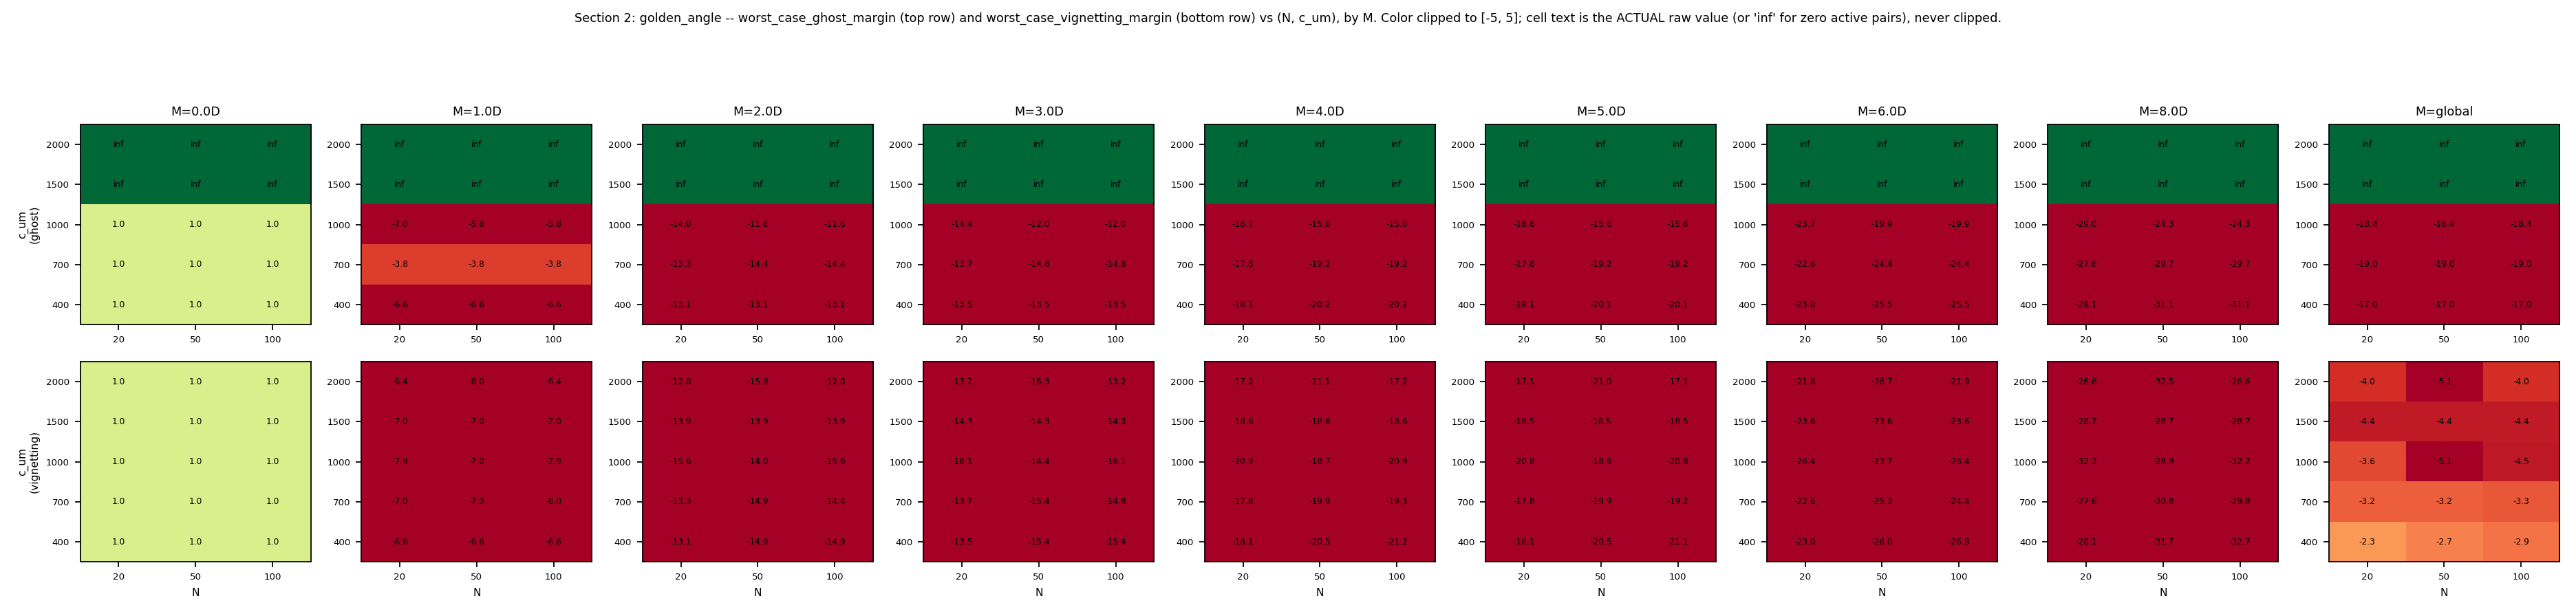
\includegraphics[width=\textwidth]{figs_exploration/section2_heatmap_golden_angle.png}
\caption{golden\_angle: worst\_case\_ghost\_margin (top row) and worst\_case\_vignetting\_margin (bottom row) vs.\ $(N, \text{c\_um})$, by $M$. axes: $N \in \{20,50,100\}$.}
\end{figure}
\begin{figure}[h!]
\centering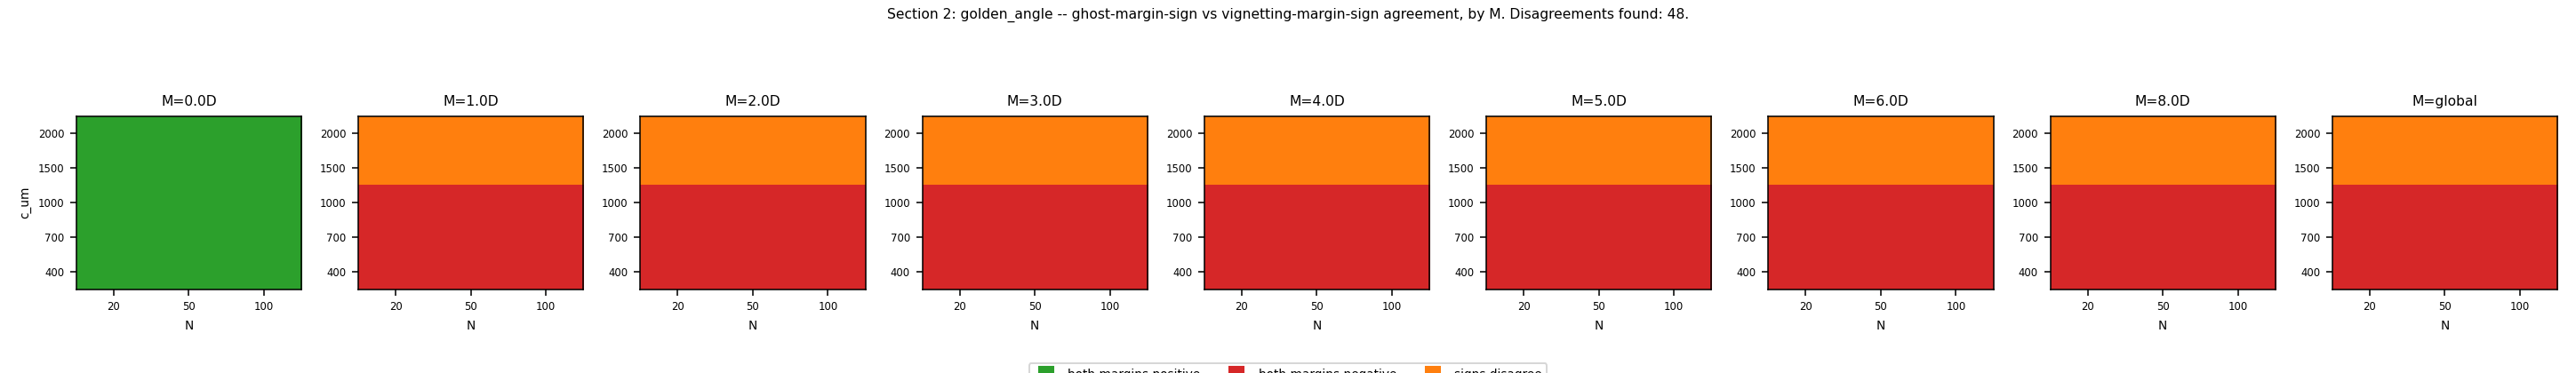
\includegraphics[width=\textwidth]{figs_exploration/section2_signagreement_golden_angle.png}
\caption{golden\_angle: ghost-margin-sign vs.\ vignetting-margin-sign agreement, by $M$ (see the figure's own title for the exact disagreement count).}
\end{figure}
\clearpage
\begin{figure}[h!]
\centering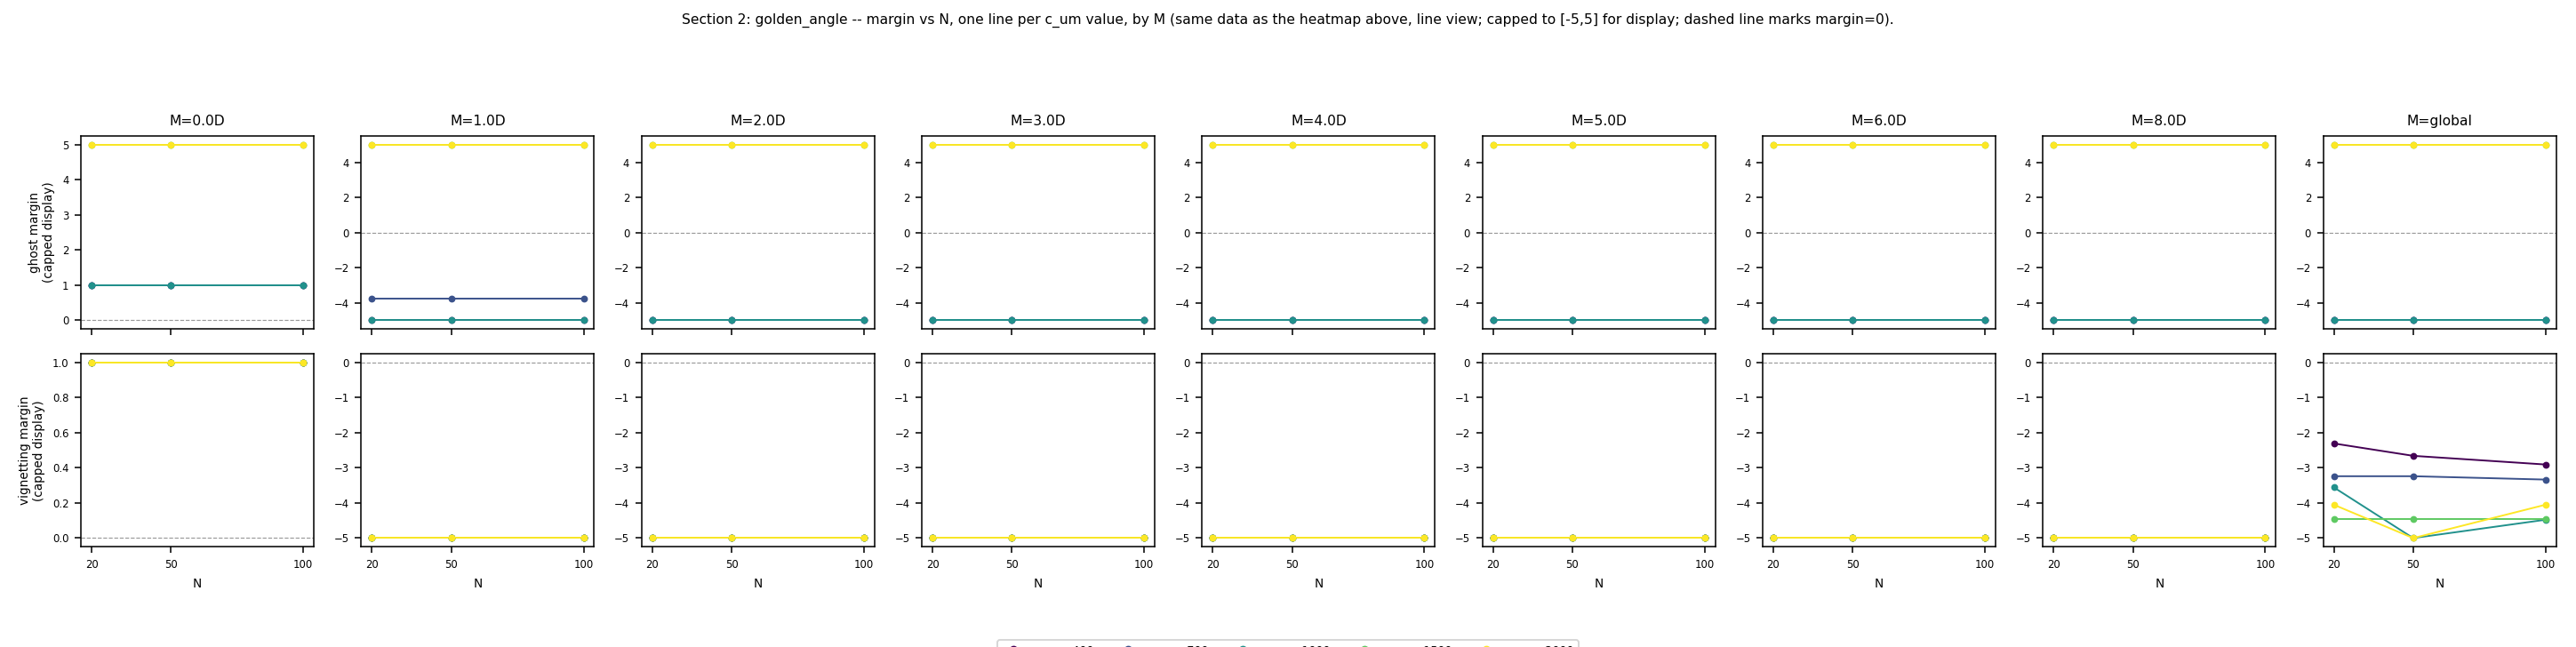
\includegraphics[width=\textwidth]{figs_exploration/section2_lineplot_golden_angle.png}
\caption{golden\_angle: same margin data as the heatmap above, shown as line plots (margin vs.\ $N$, one line per c\_um value) -- a complementary graphical view for reading trends across $N$ directly.}
\end{figure}
\clearpage
\subsection*{golden\_angle: raw number list}
\begin{longtable}{rrrrr}
\caption{golden\_angle: raw worst\_case\_ghost\_margin and worst\_case\_vignetting\_margin values behind the heatmap and line plot above -- one row per tested $(N, c\_um, M)$ point. `inf' = zero active hole pairs under the pupil at that point (structurally safe, undisplayable on a linear scale).} \\
\toprule
N & c\_um & M & ghost\_margin & vignetting\_margin \\
\midrule
\endfirsthead
\toprule
N & c\_um & M & ghost\_margin & vignetting\_margin \\
\midrule
\endhead
\midrule
\multicolumn{5}{r}{\itshape continued on next page} \\
\endfoot
\bottomrule
\endlastfoot
20 & 400 & 0D & 1.000 & 1.000 \\
20 & 400 & 1D & -6.587 & -6.587 \\
20 & 400 & 2D & -13.119 & -13.119 \\
20 & 400 & 3D & -13.536 & -13.536 \\
20 & 400 & 4D & -18.134 & -18.134 \\
20 & 400 & 5D & -18.053 & -18.053 \\
20 & 400 & 6D & -22.998 & -22.998 \\
20 & 400 & 8D & -28.057 & -28.057 \\
20 & 400 & global & -17.047 & -2.305 \\
50 & 400 & 0D & 1.000 & 1.000 \\
50 & 400 & 1D & -6.587 & -6.587 \\
50 & 400 & 2D & -13.119 & -14.928 \\
50 & 400 & 3D & -13.536 & -15.399 \\
50 & 400 & 4D & -20.164 & -20.542 \\
50 & 400 & 5D & -20.074 & -20.451 \\
50 & 400 & 6D & -25.544 & -26.018 \\
50 & 400 & 8D & -31.140 & -31.715 \\
50 & 400 & global & -17.047 & -2.657 \\
100 & 400 & 0D & 1.000 & 1.000 \\
100 & 400 & 1D & -6.587 & -6.587 \\
100 & 400 & 2D & -13.119 & -14.929 \\
100 & 400 & 3D & -13.536 & -15.400 \\
100 & 400 & 4D & -20.164 & -21.185 \\
100 & 400 & 5D & -20.074 & -21.091 \\
100 & 400 & 6D & -25.544 & -26.825 \\
100 & 400 & 8D & -31.140 & -32.691 \\
100 & 400 & global & -17.047 & -2.904 \\
20 & 700 & 0D & 1.000 & 1.000 \\
20 & 700 & 1D & -3.752 & -7.016 \\
20 & 700 & 2D & -13.310 & -13.310 \\
20 & 700 & 3D & -13.733 & -13.733 \\
20 & 700 & 4D & -17.843 & -17.843 \\
20 & 700 & 5D & -17.763 & -17.763 \\
20 & 700 & 6D & -22.633 & -22.633 \\
20 & 700 & 8D & -27.616 & -27.616 \\
20 & 700 & global & -18.952 & -3.238 \\
50 & 700 & 0D & 1.000 & 1.000 \\
50 & 700 & 1D & -3.752 & -7.268 \\
50 & 700 & 2D & -14.374 & -14.907 \\
50 & 700 & 3D & -14.829 & -15.377 \\
50 & 700 & 4D & -19.244 & -19.946 \\
50 & 700 & 5D & -19.158 & -19.857 \\
50 & 700 & 6D & -24.390 & -25.270 \\
50 & 700 & 8D & -29.743 & -30.809 \\
50 & 700 & global & -18.952 & -3.238 \\
100 & 700 & 0D & 1.000 & 1.000 \\
100 & 700 & 1D & -3.752 & -7.974 \\
100 & 700 & 2D & -14.374 & -14.386 \\
100 & 700 & 3D & -14.829 & -14.841 \\
100 & 700 & 4D & -19.244 & -19.259 \\
100 & 700 & 5D & -19.158 & -19.174 \\
100 & 700 & 6D & -24.390 & -24.410 \\
100 & 700 & 8D & -29.743 & -29.767 \\
100 & 700 & global & -18.952 & -3.333 \\
20 & 1000 & 0D & 1.000 & 1.000 \\
20 & 1000 & 1D & -7.049 & -7.932 \\
20 & 1000 & 2D & -13.978 & -15.621 \\
20 & 1000 & 3D & -14.421 & -16.112 \\
20 & 1000 & 4D & -18.722 & -20.886 \\
20 & 1000 & 5D & -18.639 & -20.793 \\
20 & 1000 & 6D & -23.736 & -26.449 \\
20 & 1000 & 8D & -28.951 & -32.237 \\
20 & 1000 & global & -18.410 & -3.556 \\
50 & 1000 & 0D & 1.000 & 1.000 \\
50 & 1000 & 1D & -5.788 & -7.038 \\
50 & 1000 & 2D & -11.632 & -13.958 \\
50 & 1000 & 3D & -12.005 & -14.401 \\
50 & 1000 & 4D & -15.633 & -18.696 \\
50 & 1000 & 5D & -15.563 & -18.613 \\
50 & 1000 & 6D & -19.861 & -23.703 \\
50 & 1000 & 8D & -24.259 & -28.912 \\
50 & 1000 & global & -18.410 & -5.086 \\
100 & 1000 & 0D & 1.000 & 1.000 \\
100 & 1000 & 1D & -5.788 & -7.932 \\
100 & 1000 & 2D & -11.632 & -15.621 \\
100 & 1000 & 3D & -12.005 & -16.112 \\
100 & 1000 & 4D & -15.633 & -20.886 \\
100 & 1000 & 5D & -15.563 & -20.793 \\
100 & 1000 & 6D & -19.861 & -26.449 \\
100 & 1000 & 8D & -24.259 & -32.237 \\
100 & 1000 & global & -18.410 & -4.478 \\
20 & 1500 & 0D & inf & 1.000 \\
20 & 1500 & 1D & inf & -6.991 \\
20 & 1500 & 2D & inf & -13.869 \\
20 & 1500 & 3D & inf & -14.309 \\
20 & 1500 & 4D & inf & -18.579 \\
20 & 1500 & 5D & inf & -18.496 \\
20 & 1500 & 6D & inf & -23.556 \\
20 & 1500 & 8D & inf & -28.734 \\
20 & 1500 & global & inf & -4.445 \\
50 & 1500 & 0D & inf & 1.000 \\
50 & 1500 & 1D & inf & -6.991 \\
50 & 1500 & 2D & inf & -13.869 \\
50 & 1500 & 3D & inf & -14.309 \\
50 & 1500 & 4D & inf & -18.579 \\
50 & 1500 & 5D & inf & -18.496 \\
50 & 1500 & 6D & inf & -23.556 \\
50 & 1500 & 8D & inf & -28.734 \\
50 & 1500 & global & inf & -4.445 \\
100 & 1500 & 0D & inf & 1.000 \\
100 & 1500 & 1D & inf & -6.991 \\
100 & 1500 & 2D & inf & -13.869 \\
100 & 1500 & 3D & inf & -14.309 \\
100 & 1500 & 4D & inf & -18.579 \\
100 & 1500 & 5D & inf & -18.496 \\
100 & 1500 & 6D & inf & -23.556 \\
100 & 1500 & 8D & inf & -28.734 \\
100 & 1500 & global & inf & -4.445 \\
20 & 2000 & 0D & inf & 1.000 \\
20 & 2000 & 1D & inf & -6.411 \\
20 & 2000 & 2D & inf & -12.791 \\
20 & 2000 & 3D & inf & -13.198 \\
20 & 2000 & 4D & inf & -17.159 \\
20 & 2000 & 5D & inf & -17.082 \\
20 & 2000 & 6D & inf & -21.775 \\
20 & 2000 & 8D & inf & -26.577 \\
20 & 2000 & global & inf & -4.050 \\
50 & 2000 & 0D & inf & 1.000 \\
50 & 2000 & 1D & inf & -8.007 \\
50 & 2000 & 2D & inf & -15.761 \\
50 & 2000 & 3D & inf & -16.256 \\
50 & 2000 & 4D & inf & -21.070 \\
50 & 2000 & 5D & inf & -20.976 \\
50 & 2000 & 6D & inf & -26.680 \\
50 & 2000 & 8D & inf & -32.516 \\
50 & 2000 & global & inf & -5.138 \\
100 & 2000 & 0D & inf & 1.000 \\
100 & 2000 & 1D & inf & -6.411 \\
100 & 2000 & 2D & inf & -12.791 \\
100 & 2000 & 3D & inf & -13.198 \\
100 & 2000 & 4D & inf & -17.159 \\
100 & 2000 & 5D & inf & -17.082 \\
100 & 2000 & 6D & inf & -21.775 \\
100 & 2000 & 8D & inf & -26.577 \\
100 & 2000 & global & inf & -4.050 \\
\end{longtable}

\clearpage

\section{hexagonal}
\begin{figure}[h!]
\centering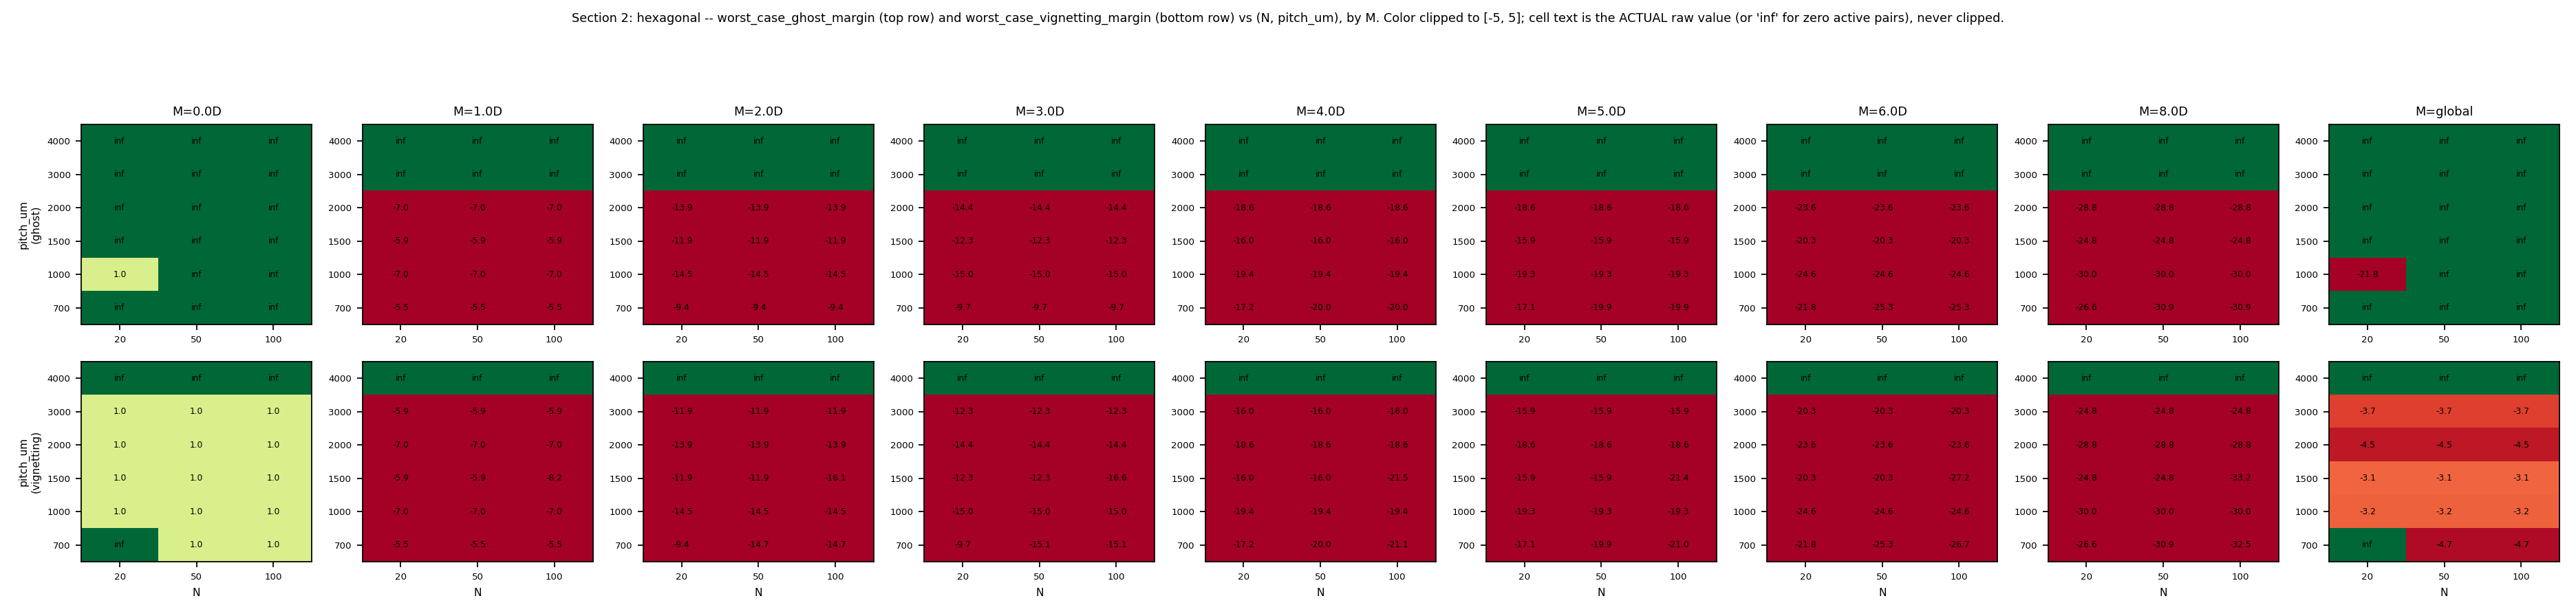
\includegraphics[width=\textwidth]{figs_exploration/section2_heatmap_hexagonal.png}
\caption{hexagonal: worst\_case\_ghost\_margin (top row) and worst\_case\_vignetting\_margin (bottom row) vs.\ $(N, \text{pitch\_um})$, by $M$. axes: $N \in \{20,50,100\}$.}
\end{figure}
\begin{figure}[h!]
\centering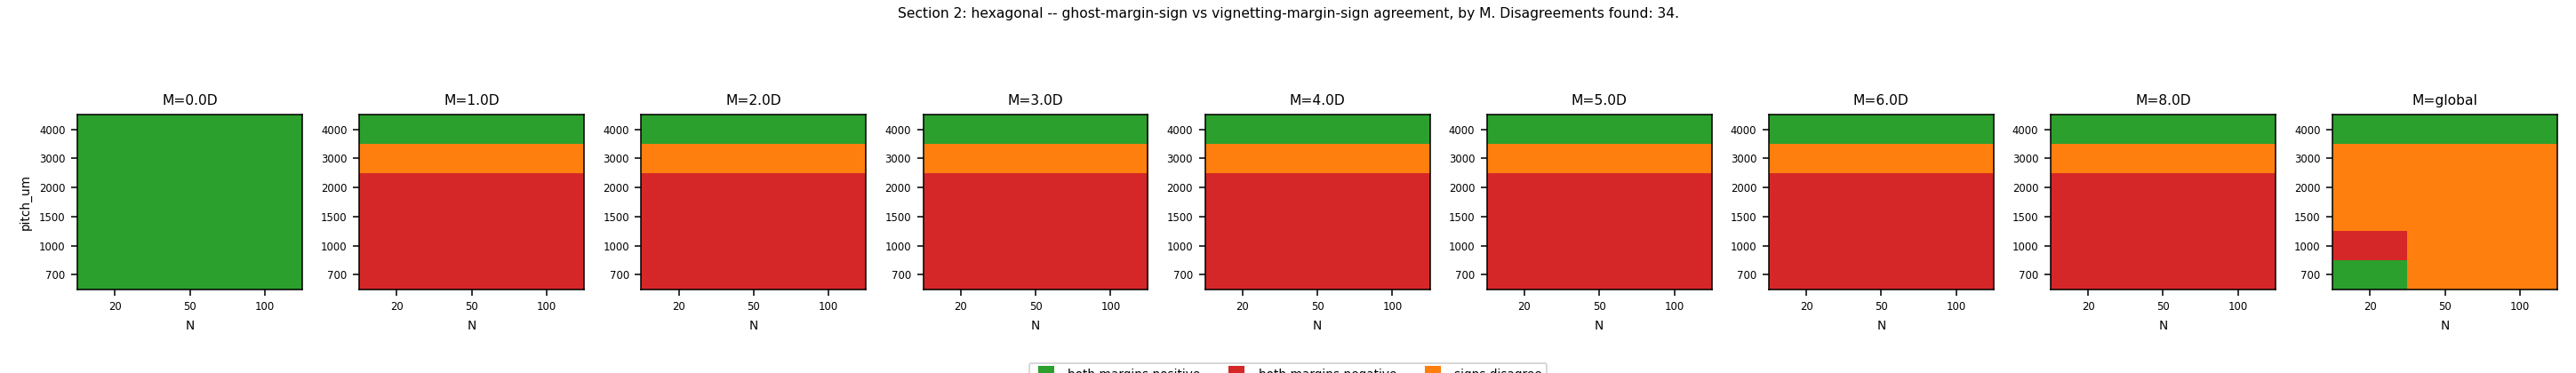
\includegraphics[width=\textwidth]{figs_exploration/section2_signagreement_hexagonal.png}
\caption{hexagonal: ghost-margin-sign vs.\ vignetting-margin-sign agreement, by $M$ (see the figure's own title for the exact disagreement count).}
\end{figure}
\clearpage
\begin{figure}[h!]
\centering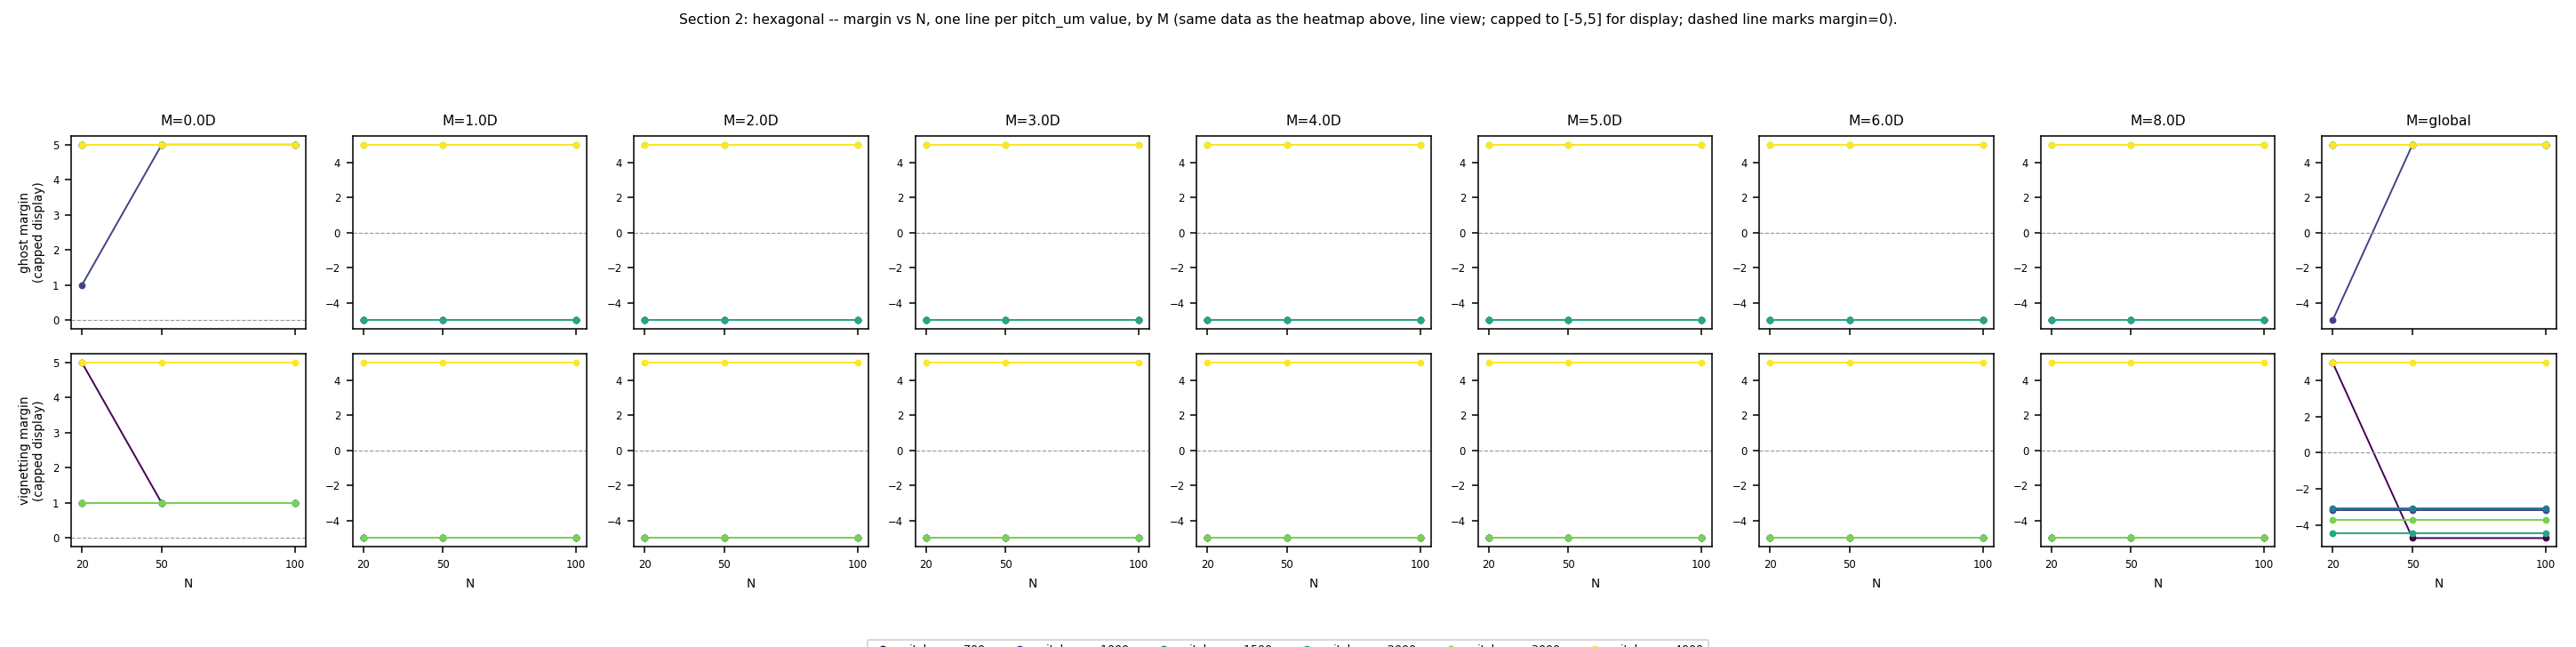
\includegraphics[width=\textwidth]{figs_exploration/section2_lineplot_hexagonal.png}
\caption{hexagonal: same margin data as the heatmap above, shown as line plots (margin vs.\ $N$, one line per pitch\_um value) -- a complementary graphical view for reading trends across $N$ directly.}
\end{figure}
\clearpage
\subsection*{hexagonal: raw number list}
\begin{longtable}{rrrrr}
\caption{hexagonal: raw worst\_case\_ghost\_margin and worst\_case\_vignetting\_margin values behind the heatmap and line plot above -- one row per tested $(N, pitch\_um, M)$ point. `inf' = zero active hole pairs under the pupil at that point (structurally safe, undisplayable on a linear scale).} \\
\toprule
N & pitch\_um & M & ghost\_margin & vignetting\_margin \\
\midrule
\endfirsthead
\toprule
N & pitch\_um & M & ghost\_margin & vignetting\_margin \\
\midrule
\endhead
\midrule
\multicolumn{5}{r}{\itshape continued on next page} \\
\endfoot
\bottomrule
\endlastfoot
20 & 700 & 0D & inf & inf \\
20 & 700 & 1D & -5.477 & -5.477 \\
20 & 700 & 2D & -9.437 & -9.437 \\
20 & 700 & 3D & -9.746 & -9.746 \\
20 & 700 & 4D & -17.181 & -17.181 \\
20 & 700 & 5D & -17.104 & -17.104 \\
20 & 700 & 6D & -21.803 & -21.803 \\
20 & 700 & 8D & -26.610 & -26.610 \\
20 & 700 & global & inf & inf \\
50 & 700 & 0D & inf & 1.000 \\
50 & 700 & 1D & -5.477 & -5.477 \\
50 & 700 & 2D & -9.437 & -14.656 \\
50 & 700 & 3D & -9.746 & -15.119 \\
50 & 700 & 4D & -19.994 & -19.994 \\
50 & 700 & 5D & -19.905 & -19.905 \\
50 & 700 & 6D & -25.330 & -25.330 \\
50 & 700 & 8D & -30.882 & -30.882 \\
50 & 700 & global & inf & -4.733 \\
100 & 700 & 0D & inf & 1.000 \\
100 & 700 & 1D & -5.477 & -5.477 \\
100 & 700 & 2D & -9.437 & -14.656 \\
100 & 700 & 3D & -9.746 & -15.119 \\
100 & 700 & 4D & -19.994 & -21.090 \\
100 & 700 & 5D & -19.905 & -20.996 \\
100 & 700 & 6D & -25.330 & -26.705 \\
100 & 700 & 8D & -30.882 & -32.546 \\
100 & 700 & global & inf & -4.733 \\
20 & 1000 & 0D & 1.000 & 1.000 \\
20 & 1000 & 1D & -7.013 & -7.013 \\
20 & 1000 & 2D & -14.520 & -14.520 \\
20 & 1000 & 3D & -14.978 & -14.978 \\
20 & 1000 & 4D & -19.435 & -19.435 \\
20 & 1000 & 5D & -19.349 & -19.349 \\
20 & 1000 & 6D & -24.630 & -24.630 \\
20 & 1000 & 8D & -30.034 & -30.034 \\
20 & 1000 & global & -21.773 & -3.170 \\
50 & 1000 & 0D & inf & 1.000 \\
50 & 1000 & 1D & -7.013 & -7.013 \\
50 & 1000 & 2D & -14.520 & -14.520 \\
50 & 1000 & 3D & -14.978 & -14.978 \\
50 & 1000 & 4D & -19.435 & -19.435 \\
50 & 1000 & 5D & -19.349 & -19.349 \\
50 & 1000 & 6D & -24.630 & -24.630 \\
50 & 1000 & 8D & -30.034 & -30.034 \\
50 & 1000 & global & inf & -3.170 \\
100 & 1000 & 0D & inf & 1.000 \\
100 & 1000 & 1D & -7.013 & -7.013 \\
100 & 1000 & 2D & -14.520 & -14.520 \\
100 & 1000 & 3D & -14.978 & -14.978 \\
100 & 1000 & 4D & -19.435 & -19.435 \\
100 & 1000 & 5D & -19.349 & -19.349 \\
100 & 1000 & 6D & -24.630 & -24.630 \\
100 & 1000 & 8D & -30.034 & -30.034 \\
100 & 1000 & global & inf & -3.170 \\
20 & 1500 & 0D & inf & 1.000 \\
20 & 1500 & 1D & -5.939 & -5.939 \\
20 & 1500 & 2D & -11.913 & -11.913 \\
20 & 1500 & 3D & -12.295 & -12.295 \\
20 & 1500 & 4D & -16.003 & -16.003 \\
20 & 1500 & 5D & -15.931 & -15.931 \\
20 & 1500 & 6D & -20.326 & -20.326 \\
20 & 1500 & 8D & -24.822 & -24.822 \\
20 & 1500 & global & inf & -3.095 \\
50 & 1500 & 0D & inf & 1.000 \\
50 & 1500 & 1D & -5.939 & -5.939 \\
50 & 1500 & 2D & -11.913 & -11.913 \\
50 & 1500 & 3D & -12.295 & -12.295 \\
50 & 1500 & 4D & -16.003 & -16.003 \\
50 & 1500 & 5D & -15.931 & -15.931 \\
50 & 1500 & 6D & -20.326 & -20.326 \\
50 & 1500 & 8D & -24.822 & -24.822 \\
50 & 1500 & global & inf & -3.095 \\
100 & 1500 & 0D & inf & 1.000 \\
100 & 1500 & 1D & -5.939 & -8.180 \\
100 & 1500 & 2D & -11.913 & -16.082 \\
100 & 1500 & 3D & -12.295 & -16.587 \\
100 & 1500 & 4D & -16.003 & -21.493 \\
100 & 1500 & 5D & -15.931 & -21.398 \\
100 & 1500 & 6D & -20.326 & -27.211 \\
100 & 1500 & 8D & -24.822 & -33.159 \\
100 & 1500 & global & inf & -3.095 \\
20 & 2000 & 0D & inf & 1.000 \\
20 & 2000 & 1D & -7.013 & -7.013 \\
20 & 2000 & 2D & -13.911 & -13.911 \\
20 & 2000 & 3D & -14.352 & -14.352 \\
20 & 2000 & 4D & -18.634 & -18.634 \\
20 & 2000 & 5D & -18.550 & -18.550 \\
20 & 2000 & 6D & -23.625 & -23.625 \\
20 & 2000 & 8D & -28.816 & -28.816 \\
20 & 2000 & global & inf & -4.460 \\
50 & 2000 & 0D & inf & 1.000 \\
50 & 2000 & 1D & -7.013 & -7.013 \\
50 & 2000 & 2D & -13.911 & -13.911 \\
50 & 2000 & 3D & -14.352 & -14.352 \\
50 & 2000 & 4D & -18.634 & -18.634 \\
50 & 2000 & 5D & -18.550 & -18.550 \\
50 & 2000 & 6D & -23.625 & -23.625 \\
50 & 2000 & 8D & -28.816 & -28.816 \\
50 & 2000 & global & inf & -4.460 \\
100 & 2000 & 0D & inf & 1.000 \\
100 & 2000 & 1D & -7.013 & -7.013 \\
100 & 2000 & 2D & -13.911 & -13.911 \\
100 & 2000 & 3D & -14.352 & -14.352 \\
100 & 2000 & 4D & -18.634 & -18.634 \\
100 & 2000 & 5D & -18.550 & -18.550 \\
100 & 2000 & 6D & -23.625 & -23.625 \\
100 & 2000 & 8D & -28.816 & -28.816 \\
100 & 2000 & global & inf & -4.460 \\
20 & 3000 & 0D & inf & 1.000 \\
20 & 3000 & 1D & inf & -5.939 \\
20 & 3000 & 2D & inf & -11.913 \\
20 & 3000 & 3D & inf & -12.295 \\
20 & 3000 & 4D & inf & -16.003 \\
20 & 3000 & 5D & inf & -15.931 \\
20 & 3000 & 6D & inf & -20.326 \\
20 & 3000 & 8D & inf & -24.822 \\
20 & 3000 & global & inf & -3.729 \\
50 & 3000 & 0D & inf & 1.000 \\
50 & 3000 & 1D & inf & -5.939 \\
50 & 3000 & 2D & inf & -11.913 \\
50 & 3000 & 3D & inf & -12.295 \\
50 & 3000 & 4D & inf & -16.003 \\
50 & 3000 & 5D & inf & -15.931 \\
50 & 3000 & 6D & inf & -20.326 \\
50 & 3000 & 8D & inf & -24.822 \\
50 & 3000 & global & inf & -3.729 \\
100 & 3000 & 0D & inf & 1.000 \\
100 & 3000 & 1D & inf & -5.939 \\
100 & 3000 & 2D & inf & -11.913 \\
100 & 3000 & 3D & inf & -12.295 \\
100 & 3000 & 4D & inf & -16.003 \\
100 & 3000 & 5D & inf & -15.931 \\
100 & 3000 & 6D & inf & -20.326 \\
100 & 3000 & 8D & inf & -24.822 \\
100 & 3000 & global & inf & -3.729 \\
20 & 4000 & 0D & inf & inf \\
20 & 4000 & 1D & inf & inf \\
20 & 4000 & 2D & inf & inf \\
20 & 4000 & 3D & inf & inf \\
20 & 4000 & 4D & inf & inf \\
20 & 4000 & 5D & inf & inf \\
20 & 4000 & 6D & inf & inf \\
20 & 4000 & 8D & inf & inf \\
20 & 4000 & global & inf & inf \\
50 & 4000 & 0D & inf & inf \\
50 & 4000 & 1D & inf & inf \\
50 & 4000 & 2D & inf & inf \\
50 & 4000 & 3D & inf & inf \\
50 & 4000 & 4D & inf & inf \\
50 & 4000 & 5D & inf & inf \\
50 & 4000 & 6D & inf & inf \\
50 & 4000 & 8D & inf & inf \\
50 & 4000 & global & inf & inf \\
100 & 4000 & 0D & inf & inf \\
100 & 4000 & 1D & inf & inf \\
100 & 4000 & 2D & inf & inf \\
100 & 4000 & 3D & inf & inf \\
100 & 4000 & 4D & inf & inf \\
100 & 4000 & 5D & inf & inf \\
100 & 4000 & 6D & inf & inf \\
100 & 4000 & 8D & inf & inf \\
100 & 4000 & global & inf & inf \\
\end{longtable}

\clearpage

\section{jittered\_lattice}
\begin{figure}[h!]
\centering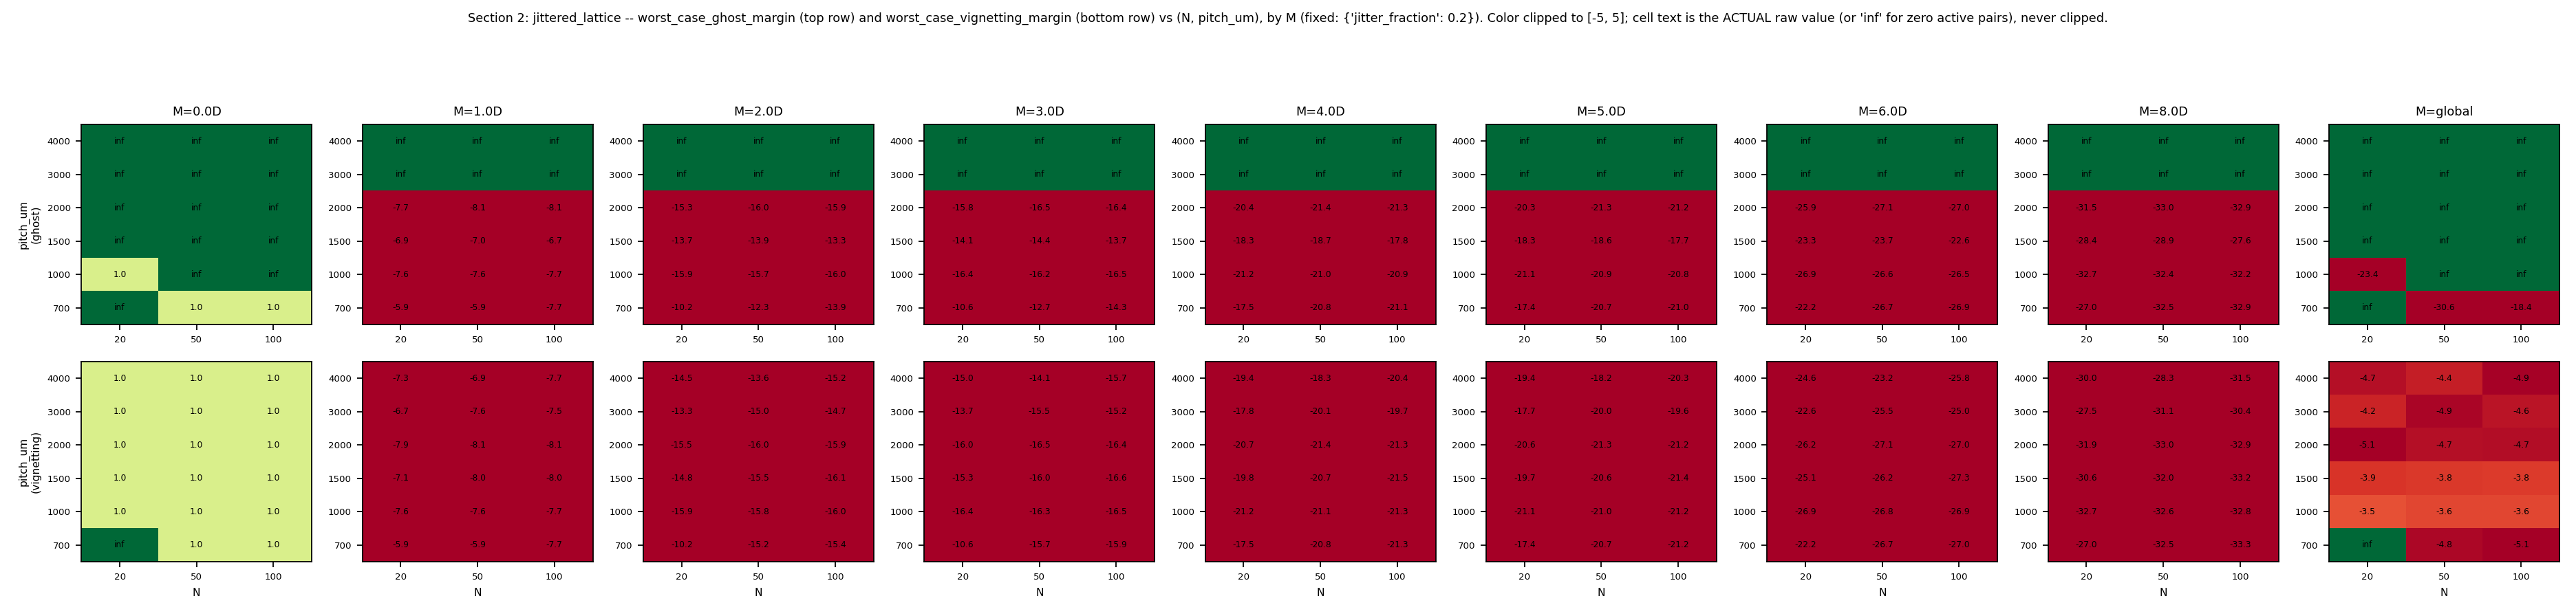
\includegraphics[width=\textwidth]{figs_exploration/section2_heatmap_jittered_lattice.png}
\caption{jittered\_lattice: worst\_case\_ghost\_margin (top row) and worst\_case\_vignetting\_margin (bottom row) vs.\ $(N, \text{pitch\_um})$, by $M$. jitter\_fraction=0.2 held fixed at its own median tested value; axes: $N \in \{20,50,100\}$.}
\end{figure}
\begin{figure}[h!]
\centering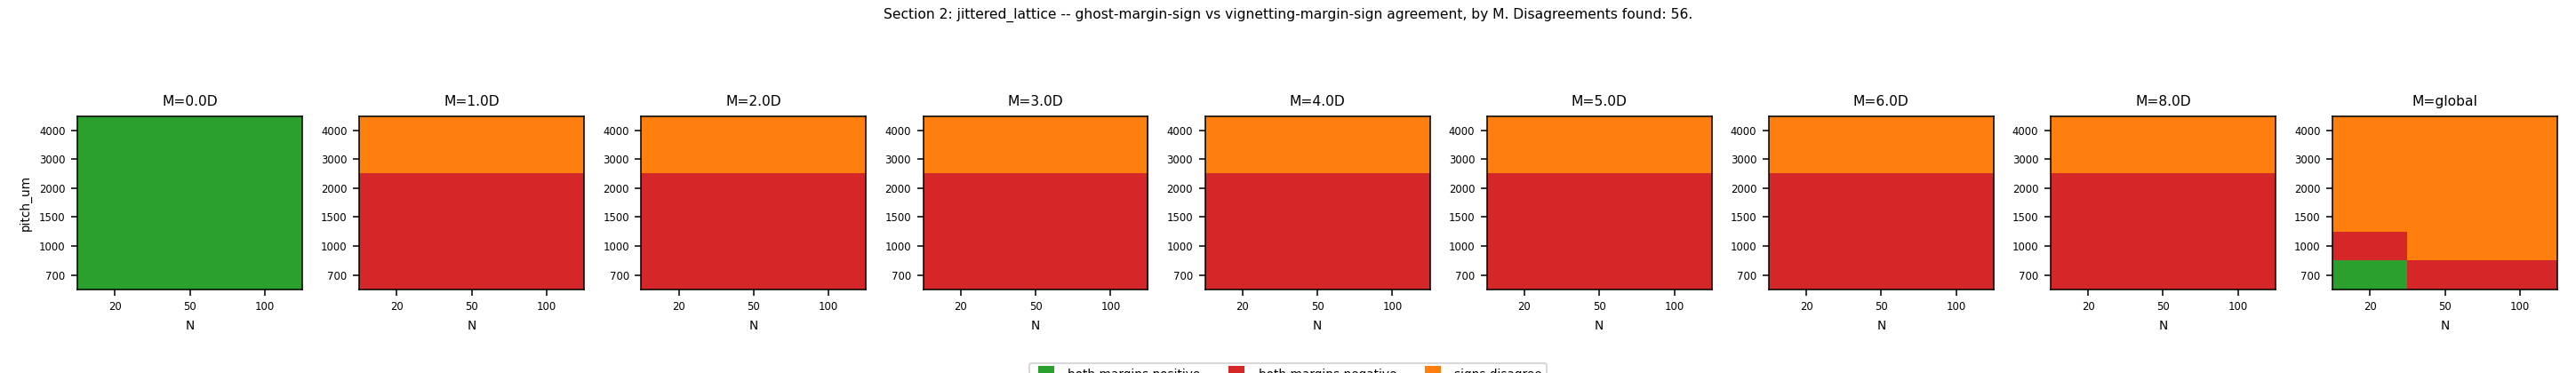
\includegraphics[width=\textwidth]{figs_exploration/section2_signagreement_jittered_lattice.png}
\caption{jittered\_lattice: ghost-margin-sign vs.\ vignetting-margin-sign agreement, by $M$ (see the figure's own title for the exact disagreement count).}
\end{figure}
\clearpage
\begin{figure}[h!]
\centering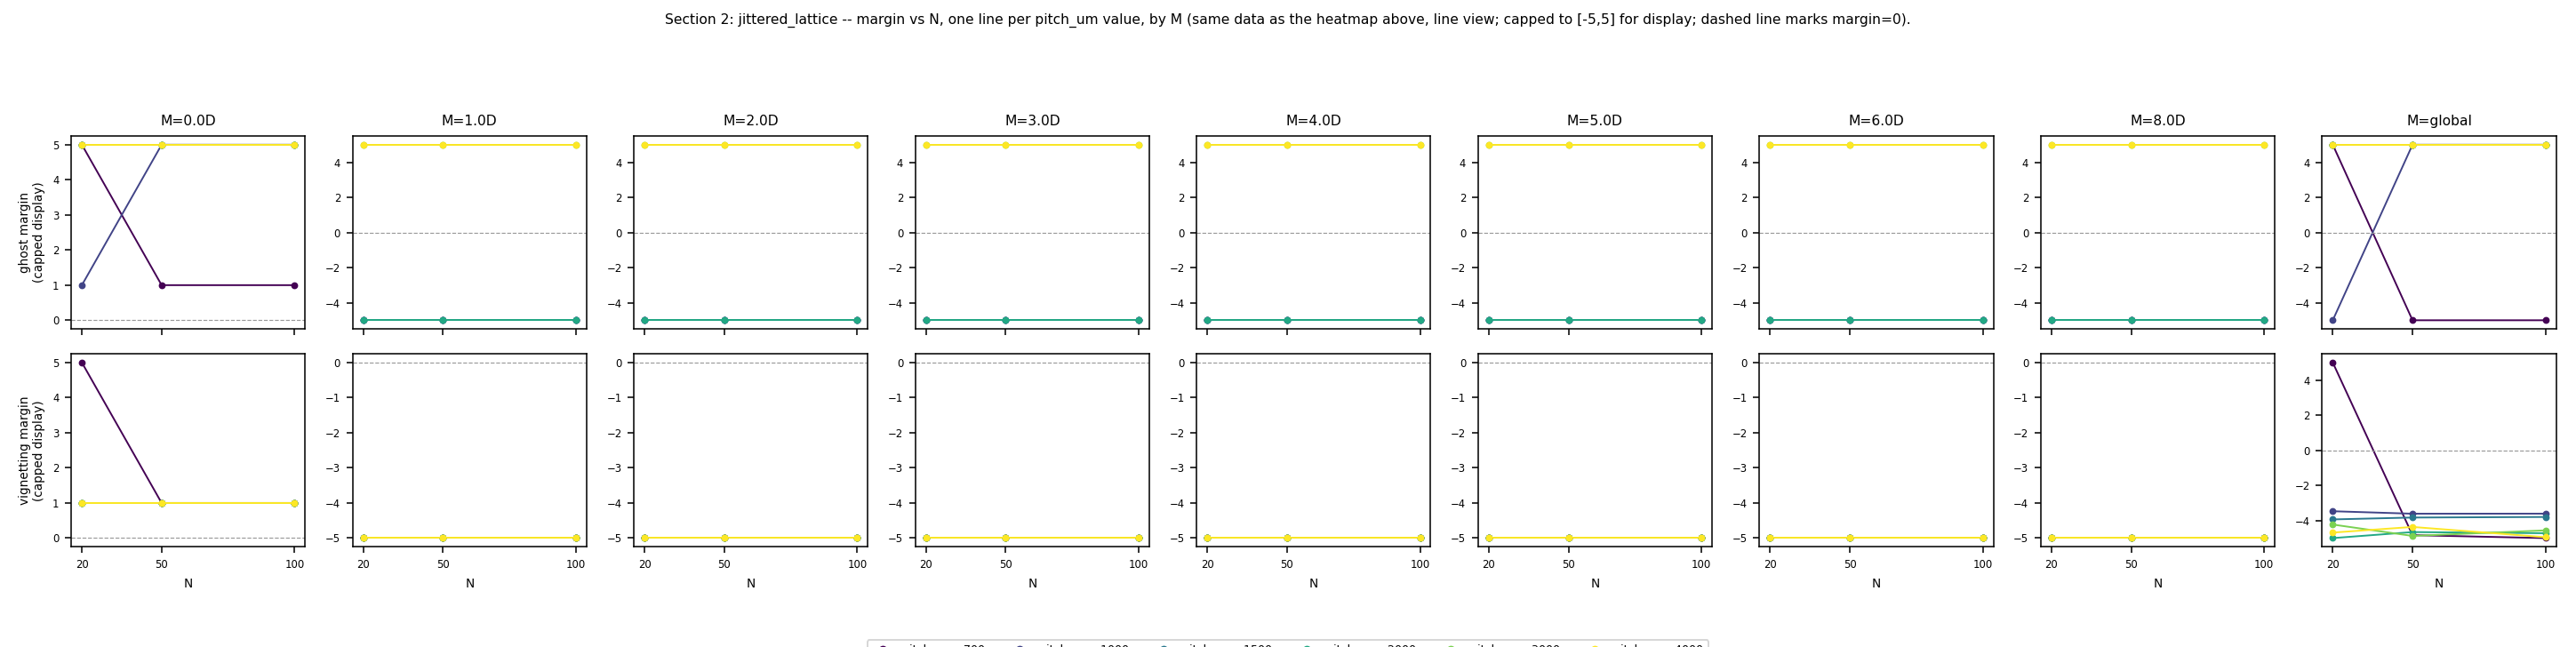
\includegraphics[width=\textwidth]{figs_exploration/section2_lineplot_jittered_lattice.png}
\caption{jittered\_lattice: same margin data as the heatmap above, shown as line plots (margin vs.\ $N$, one line per pitch\_um value) -- a complementary graphical view for reading trends across $N$ directly.}
\end{figure}
\clearpage
\subsection*{jittered\_lattice: raw number list}
\begin{longtable}{rrrrr}
\caption{jittered\_lattice: raw worst\_case\_ghost\_margin and worst\_case\_vignetting\_margin values behind the heatmap and line plot above -- one row per tested $(N, pitch\_um, M)$ point. `inf' = zero active hole pairs under the pupil at that point (structurally safe, undisplayable on a linear scale).} \\
\toprule
N & pitch\_um & M & ghost\_margin & vignetting\_margin \\
\midrule
\endfirsthead
\toprule
N & pitch\_um & M & ghost\_margin & vignetting\_margin \\
\midrule
\endhead
\midrule
\multicolumn{5}{r}{\itshape continued on next page} \\
\endfoot
\bottomrule
\endlastfoot
20 & 700 & 0D & inf & inf \\
20 & 700 & 1D & -5.944 & -5.944 \\
20 & 700 & 2D & -10.220 & -10.220 \\
20 & 700 & 3D & -10.551 & -10.551 \\
20 & 700 & 4D & -17.460 & -17.460 \\
20 & 700 & 5D & -17.382 & -17.382 \\
20 & 700 & 6D & -22.153 & -22.153 \\
20 & 700 & 8D & -27.034 & -27.034 \\
20 & 700 & global & inf & inf \\
50 & 700 & 0D & 1.000 & 1.000 \\
50 & 700 & 1D & -5.897 & -5.897 \\
50 & 700 & 2D & -12.341 & -15.225 \\
50 & 700 & 3D & -12.735 & -15.705 \\
50 & 700 & 4D & -20.772 & -20.772 \\
50 & 700 & 5D & -20.680 & -20.680 \\
50 & 700 & 6D & -26.750 & -26.750 \\
50 & 700 & 8D & -32.517 & -32.517 \\
50 & 700 & global & -30.592 & -4.833 \\
100 & 700 & 0D & 1.000 & 1.000 \\
100 & 700 & 1D & -7.668 & -7.690 \\
100 & 700 & 2D & -13.851 & -15.372 \\
100 & 700 & 3D & -14.290 & -15.856 \\
100 & 700 & 4D & -21.067 & -21.330 \\
100 & 700 & 5D & -20.974 & -21.236 \\
100 & 700 & 6D & -26.944 & -27.007 \\
100 & 700 & 8D & -32.862 & -33.320 \\
100 & 700 & global & -18.416 & -5.059 \\
20 & 1000 & 0D & 1.000 & 1.000 \\
20 & 1000 & 1D & -7.613 & -7.613 \\
20 & 1000 & 2D & -15.870 & -15.870 \\
20 & 1000 & 3D & -16.369 & -16.369 \\
20 & 1000 & 4D & -21.214 & -21.214 \\
20 & 1000 & 5D & -21.120 & -21.120 \\
20 & 1000 & 6D & -26.861 & -26.861 \\
20 & 1000 & 8D & -32.735 & -32.735 \\
20 & 1000 & global & -23.410 & -3.470 \\
50 & 1000 & 0D & inf & 1.000 \\
50 & 1000 & 1D & -7.642 & -7.642 \\
50 & 1000 & 2D & -15.709 & -15.804 \\
50 & 1000 & 3D & -16.202 & -16.300 \\
50 & 1000 & 4D & -21.001 & -21.141 \\
50 & 1000 & 5D & -20.908 & -21.047 \\
50 & 1000 & 6D & -26.594 & -26.769 \\
50 & 1000 & 8D & -32.411 & -32.624 \\
50 & 1000 & global & inf & -3.611 \\
100 & 1000 & 0D & inf & 1.000 \\
100 & 1000 & 1D & -7.670 & -7.670 \\
100 & 1000 & 2D & -15.972 & -15.972 \\
100 & 1000 & 3D & -16.474 & -16.474 \\
100 & 1000 & 4D & -20.892 & -21.258 \\
100 & 1000 & 5D & -20.799 & -21.164 \\
100 & 1000 & 6D & -26.457 & -26.916 \\
100 & 1000 & 8D & -32.246 & -32.802 \\
100 & 1000 & global & inf & -3.608 \\
20 & 1500 & 0D & inf & 1.000 \\
20 & 1500 & 1D & -6.895 & -7.127 \\
20 & 1500 & 2D & -13.692 & -14.821 \\
20 & 1500 & 3D & -14.127 & -15.289 \\
20 & 1500 & 4D & -18.346 & -19.832 \\
20 & 1500 & 5D & -18.264 & -19.744 \\
20 & 1500 & 6D & -23.264 & -25.128 \\
20 & 1500 & 8D & -28.380 & -30.637 \\
20 & 1500 & global & inf & -3.936 \\
50 & 1500 & 0D & inf & 1.000 \\
50 & 1500 & 1D & -7.026 & -7.950 \\
50 & 1500 & 2D & -13.936 & -15.495 \\
50 & 1500 & 3D & -14.378 & -15.983 \\
50 & 1500 & 4D & -18.667 & -20.720 \\
50 & 1500 & 5D & -18.584 & -20.628 \\
50 & 1500 & 6D & -23.667 & -26.241 \\
50 & 1500 & 8D & -28.867 & -31.985 \\
50 & 1500 & global & inf & -3.829 \\
100 & 1500 & 0D & inf & 1.000 \\
100 & 1500 & 1D & -6.677 & -7.975 \\
100 & 1500 & 2D & -13.286 & -16.107 \\
100 & 1500 & 3D & -13.708 & -16.613 \\
100 & 1500 & 4D & -17.811 & -21.526 \\
100 & 1500 & 5D & -17.731 & -21.430 \\
100 & 1500 & 6D & -22.592 & -27.252 \\
100 & 1500 & 8D & -27.566 & -33.209 \\
100 & 1500 & global & inf & -3.797 \\
20 & 2000 & 0D & inf & 1.000 \\
20 & 2000 & 1D & -7.743 & -7.851 \\
20 & 2000 & 2D & -15.270 & -15.471 \\
20 & 2000 & 3D & -15.751 & -15.958 \\
20 & 2000 & 4D & -20.424 & -20.688 \\
20 & 2000 & 5D & -20.333 & -20.596 \\
20 & 2000 & 6D & -25.870 & -26.202 \\
20 & 2000 & 8D & -31.535 & -31.937 \\
20 & 2000 & global & inf & -5.109 \\
50 & 2000 & 0D & inf & 1.000 \\
50 & 2000 & 1D & -8.141 & -8.141 \\
50 & 2000 & 2D & -16.011 & -16.011 \\
50 & 2000 & 3D & -16.514 & -16.514 \\
50 & 2000 & 4D & -21.399 & -21.399 \\
50 & 2000 & 5D & -21.304 & -21.304 \\
50 & 2000 & 6D & -27.093 & -27.093 \\
50 & 2000 & 8D & -33.016 & -33.016 \\
50 & 2000 & global & inf & -4.657 \\
100 & 2000 & 0D & inf & 1.000 \\
100 & 2000 & 1D & -8.104 & -8.104 \\
100 & 2000 & 2D & -15.941 & -15.941 \\
100 & 2000 & 3D & -16.442 & -16.442 \\
100 & 2000 & 4D & -21.308 & -21.308 \\
100 & 2000 & 5D & -21.213 & -21.213 \\
100 & 2000 & 6D & -26.979 & -26.979 \\
100 & 2000 & 8D & -32.877 & -32.877 \\
100 & 2000 & global & inf & -4.722 \\
20 & 3000 & 0D & inf & 1.000 \\
20 & 3000 & 1D & inf & -6.672 \\
20 & 3000 & 2D & inf & -13.277 \\
20 & 3000 & 3D & inf & -13.699 \\
20 & 3000 & 4D & inf & -17.800 \\
20 & 3000 & 5D & inf & -17.720 \\
20 & 3000 & 6D & inf & -22.579 \\
20 & 3000 & 8D & inf & -27.550 \\
20 & 3000 & global & inf & -4.228 \\
50 & 3000 & 0D & inf & 1.000 \\
50 & 3000 & 1D & inf & -7.624 \\
50 & 3000 & 2D & inf & -15.049 \\
50 & 3000 & 3D & inf & -15.523 \\
50 & 3000 & 4D & inf & -20.132 \\
50 & 3000 & 5D & inf & -20.043 \\
50 & 3000 & 6D & inf & -25.504 \\
50 & 3000 & 8D & inf & -31.092 \\
50 & 3000 & global & inf & -4.877 \\
100 & 3000 & 0D & inf & 1.000 \\
100 & 3000 & 1D & inf & -7.450 \\
100 & 3000 & 2D & inf & -14.725 \\
100 & 3000 & 3D & inf & -15.190 \\
100 & 3000 & 4D & inf & -19.706 \\
100 & 3000 & 5D & inf & -19.618 \\
100 & 3000 & 6D & inf & -24.969 \\
100 & 3000 & 8D & inf & -30.444 \\
100 & 3000 & global & inf & -4.561 \\
20 & 4000 & 0D & inf & 1.000 \\
20 & 4000 & 1D & inf & -7.344 \\
20 & 4000 & 2D & inf & -14.527 \\
20 & 4000 & 3D & inf & -14.986 \\
20 & 4000 & 4D & inf & -19.445 \\
20 & 4000 & 5D & inf & -19.358 \\
20 & 4000 & 6D & inf & -24.642 \\
20 & 4000 & 8D & inf & -30.049 \\
20 & 4000 & global & inf & -4.686 \\
50 & 4000 & 0D & inf & 1.000 \\
50 & 4000 & 1D & inf & -6.873 \\
50 & 4000 & 2D & inf & -13.650 \\
50 & 4000 & 3D & inf & -14.083 \\
50 & 4000 & 4D & inf & -18.290 \\
50 & 4000 & 5D & inf & -18.208 \\
50 & 4000 & 6D & inf & -23.194 \\
50 & 4000 & 8D & inf & -28.295 \\
50 & 4000 & global & inf & -4.365 \\
100 & 4000 & 0D & inf & 1.000 \\
100 & 4000 & 1D & inf & -7.730 \\
100 & 4000 & 2D & inf & -15.245 \\
100 & 4000 & 3D & inf & -15.726 \\
100 & 4000 & 4D & inf & -20.391 \\
100 & 4000 & 5D & inf & -20.301 \\
100 & 4000 & 6D & inf & -25.829 \\
100 & 4000 & 8D & inf & -31.485 \\
100 & 4000 & global & inf & -4.949 \\
\end{longtable}

\clearpage

\section{poisson\_disk}
\begin{figure}[h!]
\centering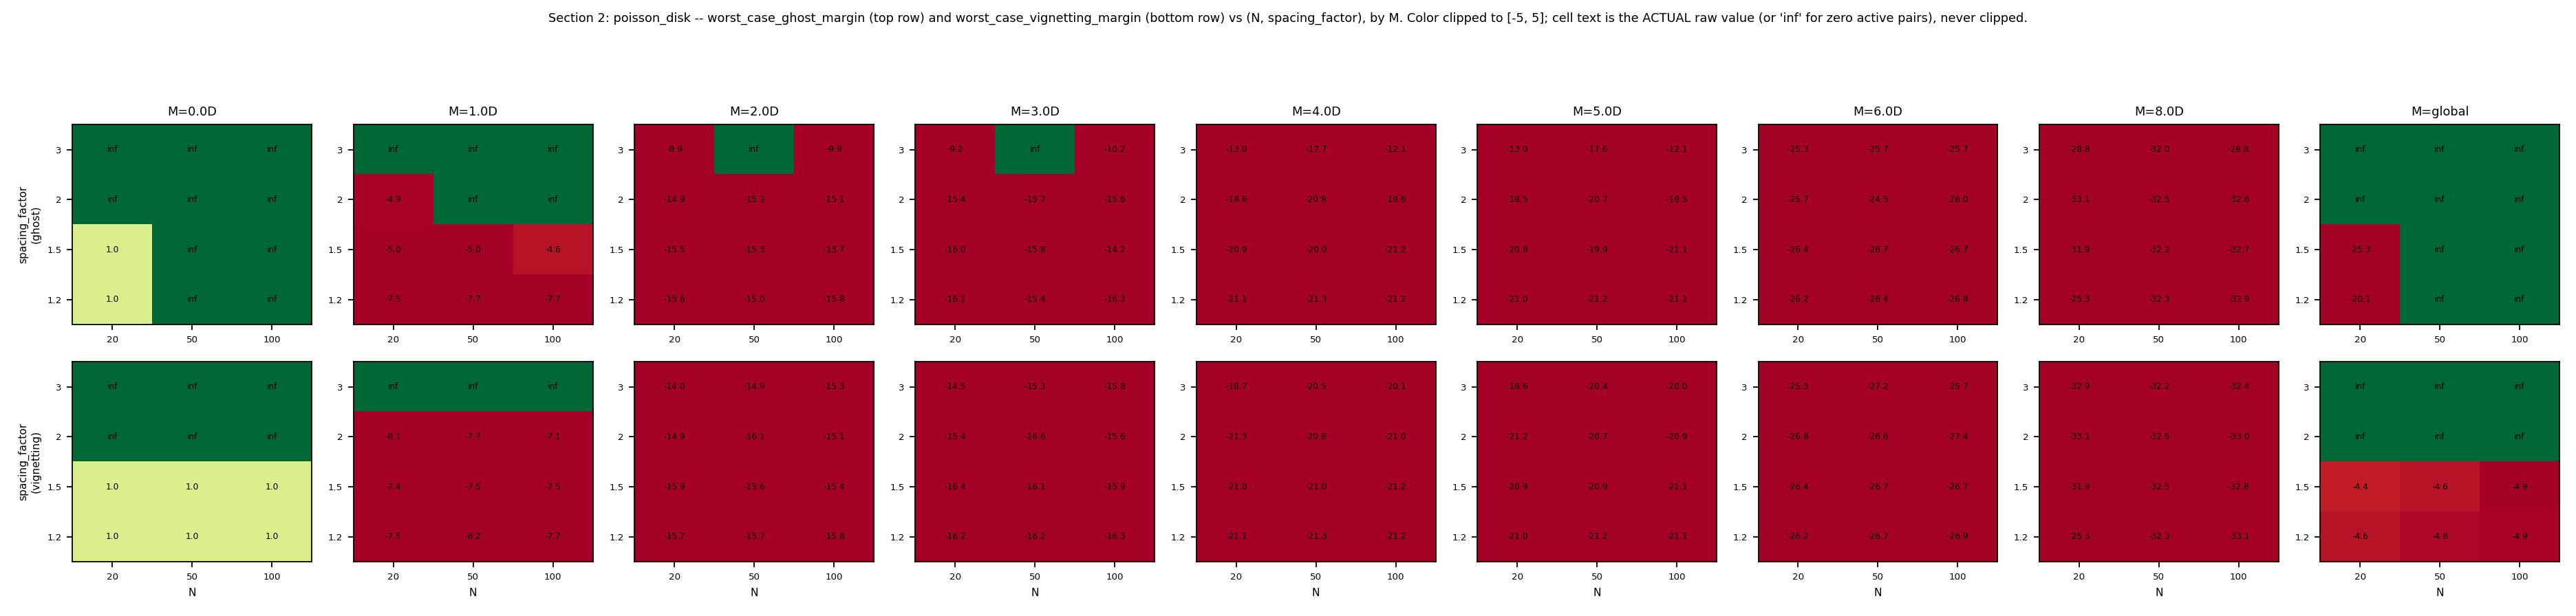
\includegraphics[width=\textwidth]{figs_exploration/section2_heatmap_poisson_disk.png}
\caption{poisson\_disk: worst\_case\_ghost\_margin (top row) and worst\_case\_vignetting\_margin (bottom row) vs.\ $(N, \text{spacing\_factor})$, by $M$. axes: $N \in \{20,50,100\}$.}
\end{figure}
\begin{figure}[h!]
\centering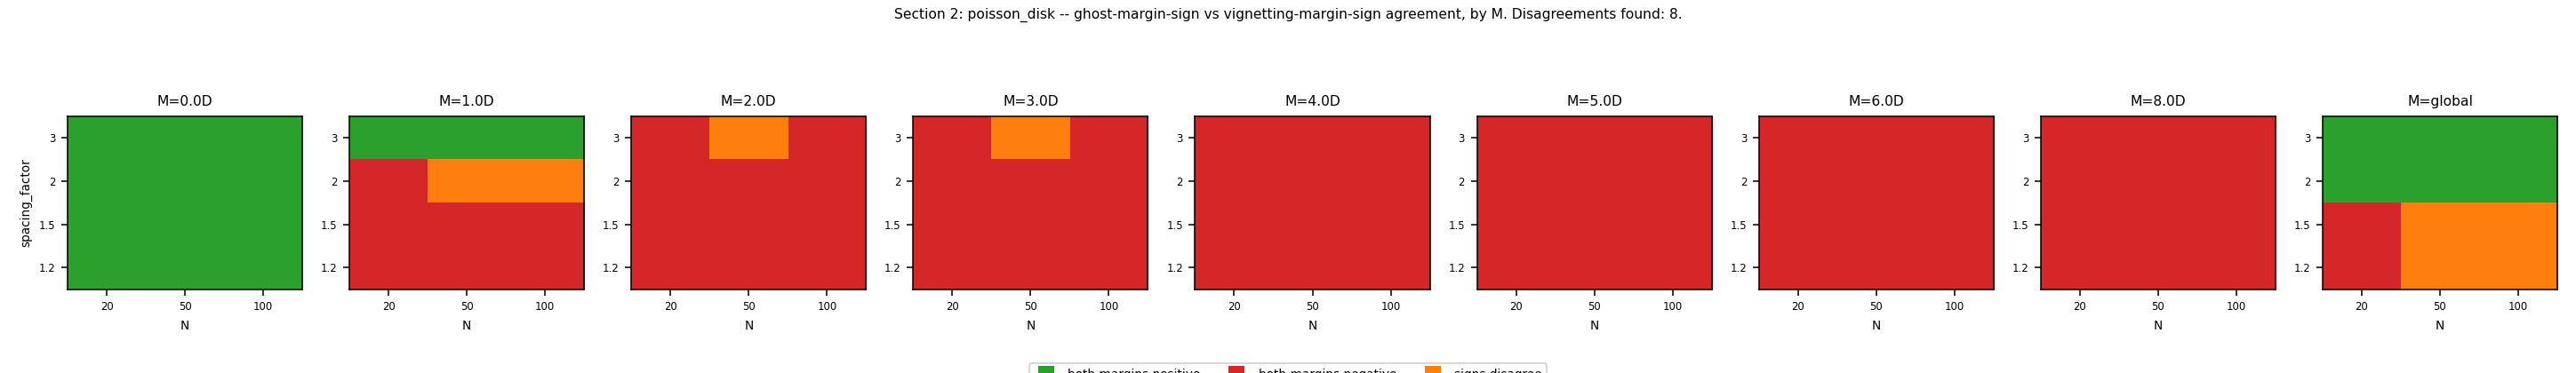
\includegraphics[width=\textwidth]{figs_exploration/section2_signagreement_poisson_disk.png}
\caption{poisson\_disk: ghost-margin-sign vs.\ vignetting-margin-sign agreement, by $M$ (see the figure's own title for the exact disagreement count).}
\end{figure}
\clearpage
\begin{figure}[h!]
\centering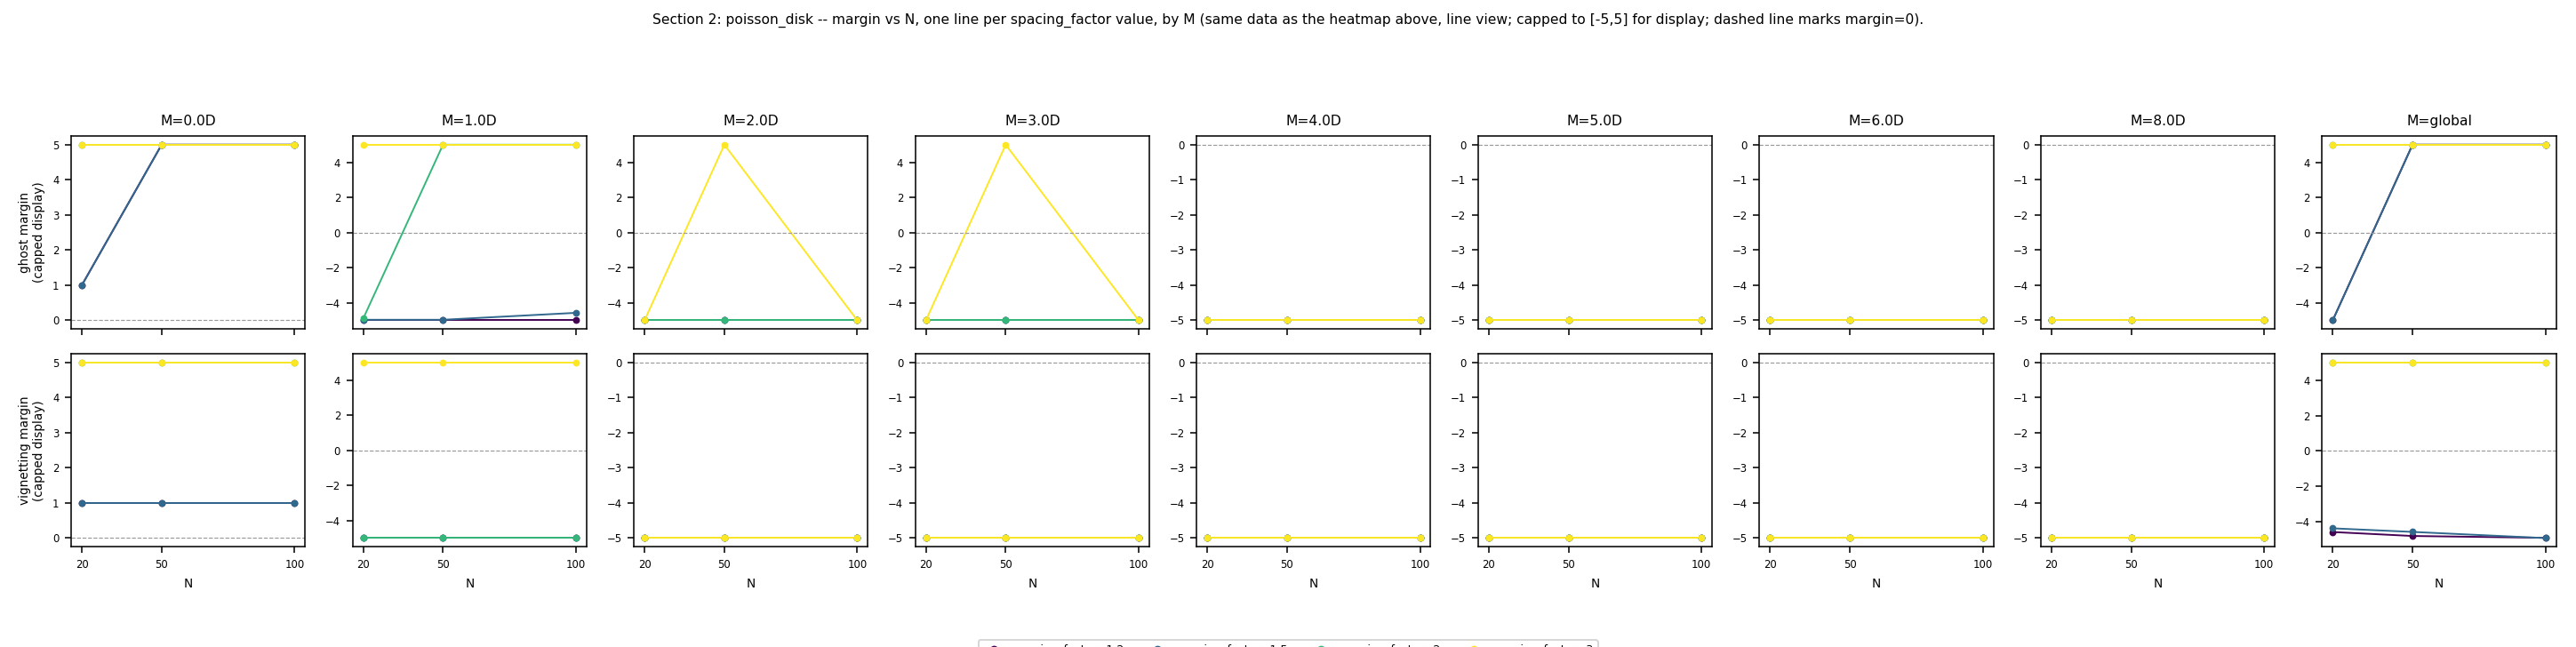
\includegraphics[width=\textwidth]{figs_exploration/section2_lineplot_poisson_disk.png}
\caption{poisson\_disk: same margin data as the heatmap above, shown as line plots (margin vs.\ $N$, one line per spacing\_factor value) -- a complementary graphical view for reading trends across $N$ directly.}
\end{figure}
\clearpage
\subsection*{poisson\_disk: raw number list}
\begin{longtable}{rrrrr}
\caption{poisson\_disk: raw worst\_case\_ghost\_margin and worst\_case\_vignetting\_margin values behind the heatmap and line plot above -- one row per tested $(N, spacing\_factor, M)$ point. `inf' = zero active hole pairs under the pupil at that point (structurally safe, undisplayable on a linear scale).} \\
\toprule
N & spacing\_factor & M & ghost\_margin & vignetting\_margin \\
\midrule
\endfirsthead
\toprule
N & spacing\_factor & M & ghost\_margin & vignetting\_margin \\
\midrule
\endhead
\midrule
\multicolumn{5}{r}{\itshape continued on next page} \\
\endfoot
\bottomrule
\endlastfoot
20 & 1.2 & 0D & 1.000 & 1.000 \\
20 & 1.2 & 1D & -7.544 & -7.544 \\
20 & 1.2 & 2D & -15.610 & -15.732 \\
20 & 1.2 & 3D & -16.101 & -16.227 \\
20 & 1.2 & 4D & -21.106 & -21.106 \\
20 & 1.2 & 5D & -21.012 & -21.012 \\
20 & 1.2 & 6D & -26.188 & -26.188 \\
20 & 1.2 & 8D & -25.336 & -25.336 \\
20 & 1.2 & global & -20.074 & -4.584 \\
50 & 1.2 & 0D & inf & 1.000 \\
50 & 1.2 & 1D & -7.698 & -8.164 \\
50 & 1.2 & 2D & -14.958 & -15.722 \\
50 & 1.2 & 3D & -15.430 & -16.217 \\
50 & 1.2 & 4D & -21.253 & -21.253 \\
50 & 1.2 & 5D & -21.159 & -21.159 \\
50 & 1.2 & 6D & -26.385 & -26.673 \\
50 & 1.2 & 8D & -32.283 & -32.283 \\
50 & 1.2 & global & inf & -4.808 \\
100 & 1.2 & 0D & inf & 1.000 \\
100 & 1.2 & 1D & -7.674 & -7.674 \\
100 & 1.2 & 2D & -15.840 & -15.840 \\
100 & 1.2 & 3D & -16.338 & -16.338 \\
100 & 1.2 & 4D & -21.234 & -21.234 \\
100 & 1.2 & 5D & -21.139 & -21.139 \\
100 & 1.2 & 6D & -26.796 & -26.922 \\
100 & 1.2 & 8D & -32.879 & -33.130 \\
100 & 1.2 & global & inf & -4.912 \\
20 & 1.5 & 0D & 1.000 & 1.000 \\
20 & 1.5 & 1D & -4.972 & -7.367 \\
20 & 1.5 & 2D & -15.469 & -15.930 \\
20 & 1.5 & 3D & -15.956 & -16.430 \\
20 & 1.5 & 4D & -20.871 & -21.032 \\
20 & 1.5 & 5D & -20.778 & -20.939 \\
20 & 1.5 & 6D & -26.356 & -26.356 \\
20 & 1.5 & 8D & -31.920 & -31.920 \\
20 & 1.5 & global & -25.343 & -4.375 \\
50 & 1.5 & 0D & inf & 1.000 \\
50 & 1.5 & 1D & -4.972 & -7.492 \\
50 & 1.5 & 2D & -15.299 & -15.584 \\
50 & 1.5 & 3D & -15.781 & -16.074 \\
50 & 1.5 & 4D & -20.013 & -21.019 \\
50 & 1.5 & 5D & -19.924 & -20.926 \\
50 & 1.5 & 6D & -26.725 & -26.725 \\
50 & 1.5 & 8D & -32.158 & -32.507 \\
50 & 1.5 & global & inf & -4.578 \\
100 & 1.5 & 0D & inf & 1.000 \\
100 & 1.5 & 1D & -4.577 & -7.527 \\
100 & 1.5 & 2D & -13.725 & -15.409 \\
100 & 1.5 & 3D & -14.160 & -15.894 \\
100 & 1.5 & 4D & -21.174 & -21.174 \\
100 & 1.5 & 5D & -21.080 & -21.080 \\
100 & 1.5 & 6D & -26.687 & -26.687 \\
100 & 1.5 & 8D & -32.656 & -32.808 \\
100 & 1.5 & global & inf & -4.927 \\
20 & 2 & 0D & inf & inf \\
20 & 2 & 1D & -4.899 & -8.085 \\
20 & 2 & 2D & -14.900 & -14.900 \\
20 & 2 & 3D & -15.370 & -15.370 \\
20 & 2 & 4D & -18.631 & -21.313 \\
20 & 2 & 5D & -18.547 & -21.218 \\
20 & 2 & 6D & -25.733 & -26.830 \\
20 & 2 & 8D & -33.081 & -33.081 \\
20 & 2 & global & inf & inf \\
50 & 2 & 0D & inf & inf \\
50 & 2 & 1D & inf & -7.742 \\
50 & 2 & 2D & -15.185 & -16.053 \\
50 & 2 & 3D & -15.663 & -16.557 \\
50 & 2 & 4D & -20.763 & -20.842 \\
50 & 2 & 5D & -20.670 & -20.749 \\
50 & 2 & 6D & -24.487 & -26.590 \\
50 & 2 & 8D & -32.491 & -32.582 \\
50 & 2 & global & inf & inf \\
100 & 2 & 0D & inf & inf \\
100 & 2 & 1D & inf & -7.110 \\
100 & 2 & 2D & -15.142 & -15.142 \\
100 & 2 & 3D & -15.619 & -15.619 \\
100 & 2 & 4D & -18.631 & -20.980 \\
100 & 2 & 5D & -18.547 & -20.886 \\
100 & 2 & 6D & -25.984 & -27.380 \\
100 & 2 & 8D & -32.630 & -33.032 \\
100 & 2 & global & inf & inf \\
20 & 3 & 0D & inf & inf \\
20 & 3 & 1D & inf & inf \\
20 & 3 & 2D & -8.880 & -14.037 \\
20 & 3 & 3D & -9.172 & -14.482 \\
20 & 3 & 4D & -13.048 & -18.683 \\
20 & 3 & 5D & -12.989 & -18.599 \\
20 & 3 & 6D & -25.259 & -25.259 \\
20 & 3 & 8D & -28.812 & -32.885 \\
20 & 3 & global & inf & inf \\
50 & 3 & 0D & inf & inf \\
50 & 3 & 1D & inf & inf \\
50 & 3 & 2D & inf & -14.854 \\
50 & 3 & 3D & inf & -15.322 \\
50 & 3 & 4D & -17.721 & -20.484 \\
50 & 3 & 5D & -17.642 & -20.393 \\
50 & 3 & 6D & -25.729 & -27.163 \\
50 & 3 & 8D & -32.049 & -32.169 \\
50 & 3 & global & inf & inf \\
100 & 3 & 0D & inf & inf \\
100 & 3 & 1D & inf & inf \\
100 & 3 & 2D & -9.917 & -15.300 \\
100 & 3 & 3D & -10.240 & -15.782 \\
100 & 3 & 4D & -12.118 & -20.059 \\
100 & 3 & 5D & -12.062 & -19.970 \\
100 & 3 & 6D & -25.658 & -25.658 \\
100 & 3 & 8D & -28.812 & -32.379 \\
100 & 3 & global & inf & inf \\
\end{longtable}

\clearpage

\section{rectangular}
\begin{figure}[h!]
\centering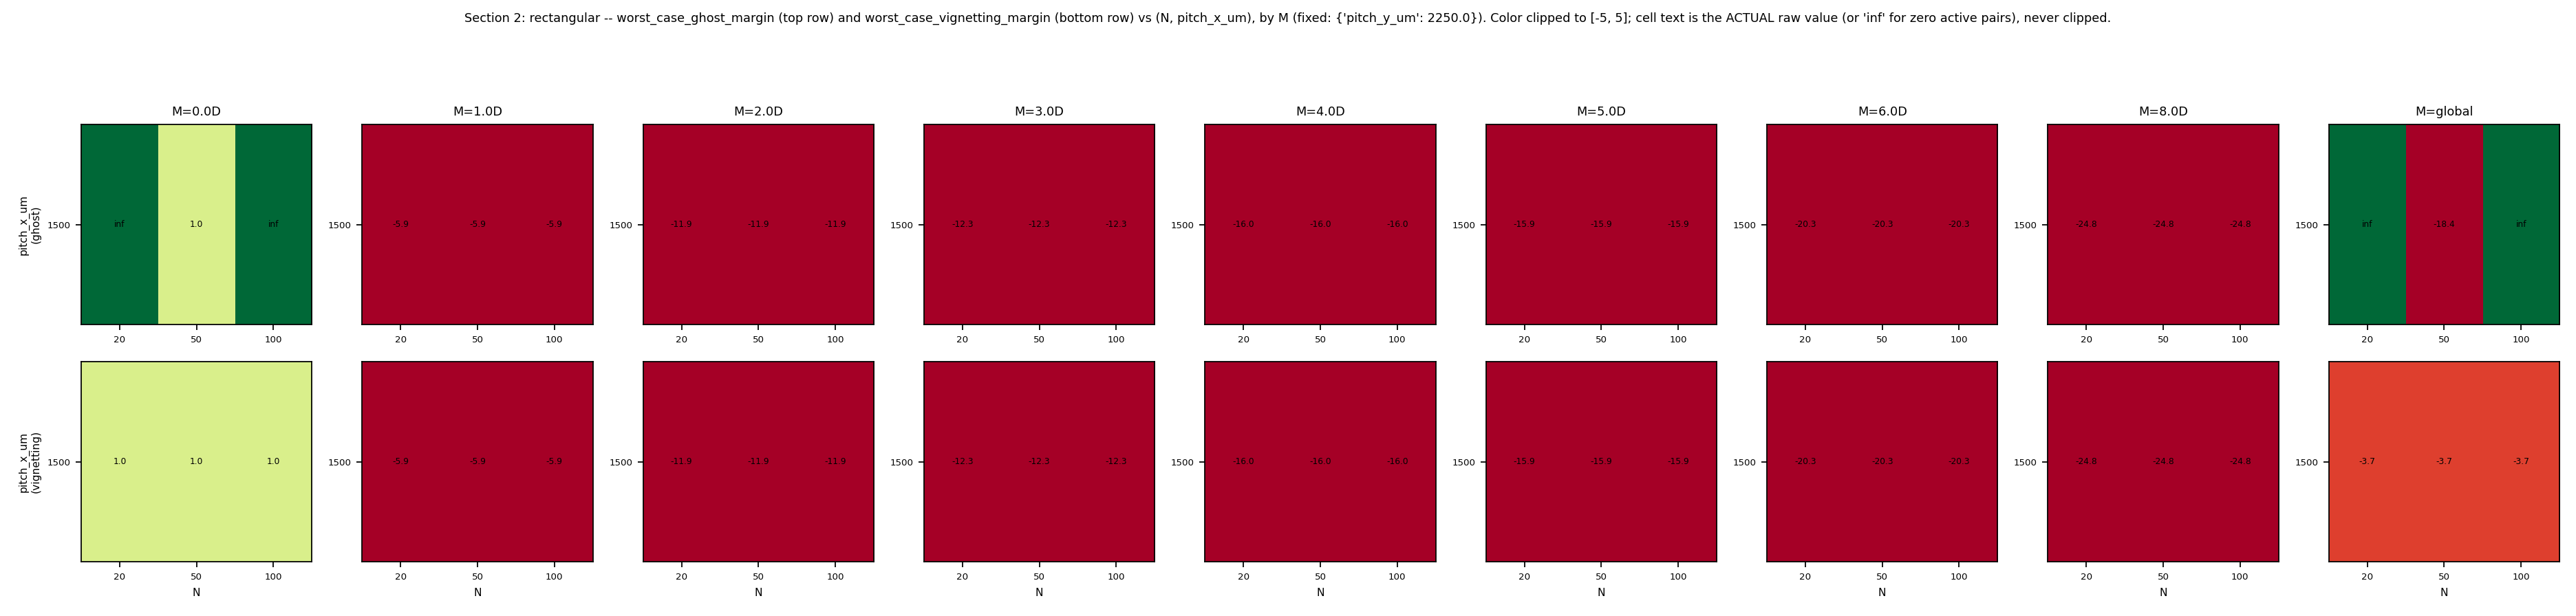
\includegraphics[width=\textwidth]{figs_exploration/section2_heatmap_rectangular.png}
\caption{rectangular: worst\_case\_ghost\_margin (top row) and worst\_case\_vignetting\_margin (bottom row) vs.\ $(N, \text{pitch\_x\_um})$, by $M$. pitch\_y\_um=2250.0 held fixed at its own median tested value; axes: $N \in \{20,50,100\}$.}
\end{figure}
\begin{figure}[h!]
\centering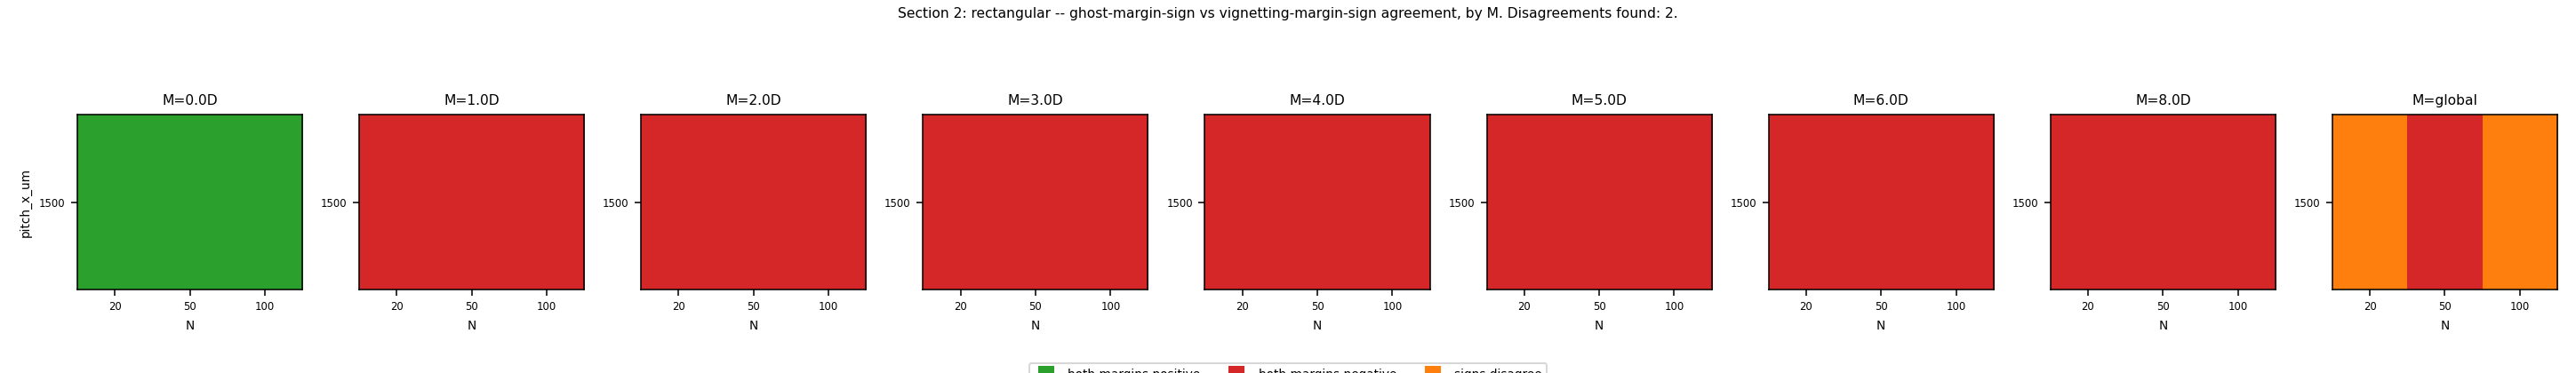
\includegraphics[width=\textwidth]{figs_exploration/section2_signagreement_rectangular.png}
\caption{rectangular: ghost-margin-sign vs.\ vignetting-margin-sign agreement, by $M$ (see the figure's own title for the exact disagreement count).}
\end{figure}
\clearpage
\begin{figure}[h!]
\centering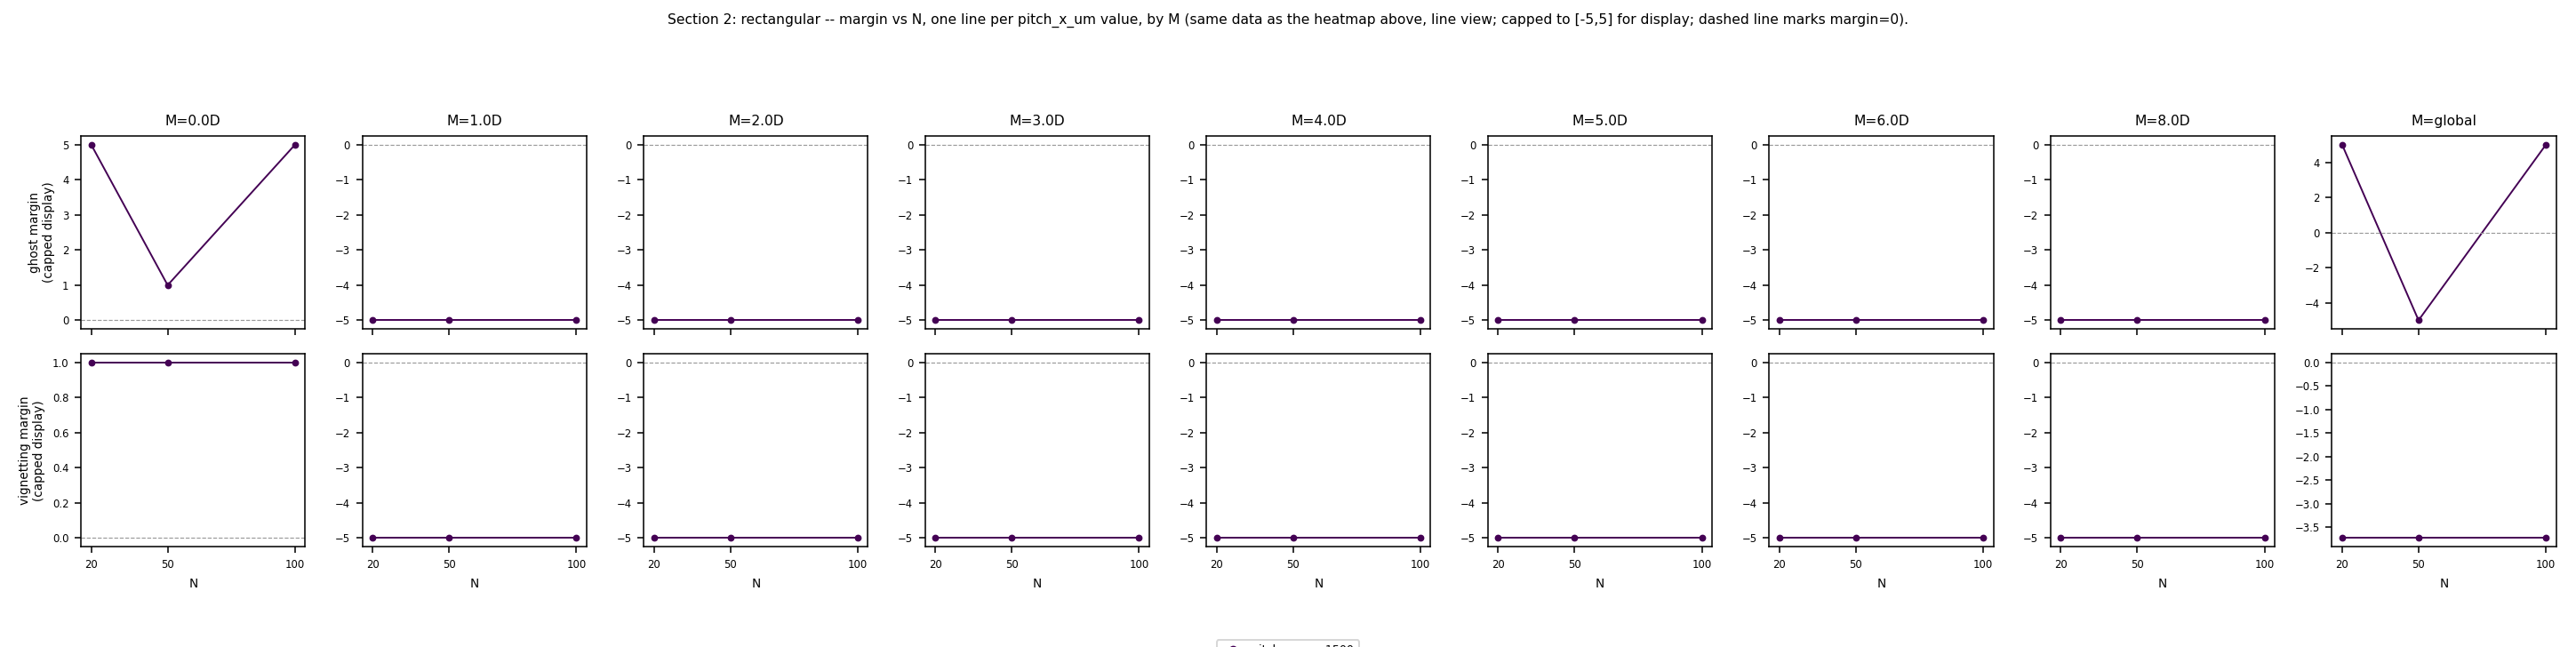
\includegraphics[width=\textwidth]{figs_exploration/section2_lineplot_rectangular.png}
\caption{rectangular: same margin data as the heatmap above, shown as line plots (margin vs.\ $N$, one line per pitch\_x\_um value) -- a complementary graphical view for reading trends across $N$ directly.}
\end{figure}
\clearpage
\subsection*{rectangular: raw number list}
\begin{longtable}{rrrrr}
\caption{rectangular: raw worst\_case\_ghost\_margin and worst\_case\_vignetting\_margin values behind the heatmap and line plot above -- one row per tested $(N, pitch\_x\_um, M)$ point. `inf' = zero active hole pairs under the pupil at that point (structurally safe, undisplayable on a linear scale).} \\
\toprule
N & pitch\_x\_um & M & ghost\_margin & vignetting\_margin \\
\midrule
\endfirsthead
\toprule
N & pitch\_x\_um & M & ghost\_margin & vignetting\_margin \\
\midrule
\endhead
\midrule
\multicolumn{5}{r}{\itshape continued on next page} \\
\endfoot
\bottomrule
\endlastfoot
20 & 1500 & 0D & inf & 1.000 \\
20 & 1500 & 1D & -5.939 & -5.939 \\
20 & 1500 & 2D & -11.913 & -11.913 \\
20 & 1500 & 3D & -12.295 & -12.295 \\
20 & 1500 & 4D & -16.003 & -16.003 \\
20 & 1500 & 5D & -15.931 & -15.931 \\
20 & 1500 & 6D & -20.326 & -20.326 \\
20 & 1500 & 8D & -24.822 & -24.822 \\
20 & 1500 & global & inf & -3.729 \\
50 & 1500 & 0D & 1.000 & 1.000 \\
50 & 1500 & 1D & -5.939 & -5.939 \\
50 & 1500 & 2D & -11.913 & -11.913 \\
50 & 1500 & 3D & -12.295 & -12.295 \\
50 & 1500 & 4D & -16.003 & -16.003 \\
50 & 1500 & 5D & -15.931 & -15.931 \\
50 & 1500 & 6D & -20.326 & -20.326 \\
50 & 1500 & 8D & -24.822 & -24.822 \\
50 & 1500 & global & -18.366 & -3.729 \\
100 & 1500 & 0D & inf & 1.000 \\
100 & 1500 & 1D & -5.939 & -5.939 \\
100 & 1500 & 2D & -11.913 & -11.913 \\
100 & 1500 & 3D & -12.295 & -12.295 \\
100 & 1500 & 4D & -16.003 & -16.003 \\
100 & 1500 & 5D & -15.931 & -15.931 \\
100 & 1500 & 6D & -20.326 & -20.326 \\
100 & 1500 & 8D & -24.822 & -24.822 \\
100 & 1500 & global & inf & -3.729 \\
\end{longtable}

\clearpage

\section{ring\_offset\_concentric}
\begin{figure}[h!]
\centering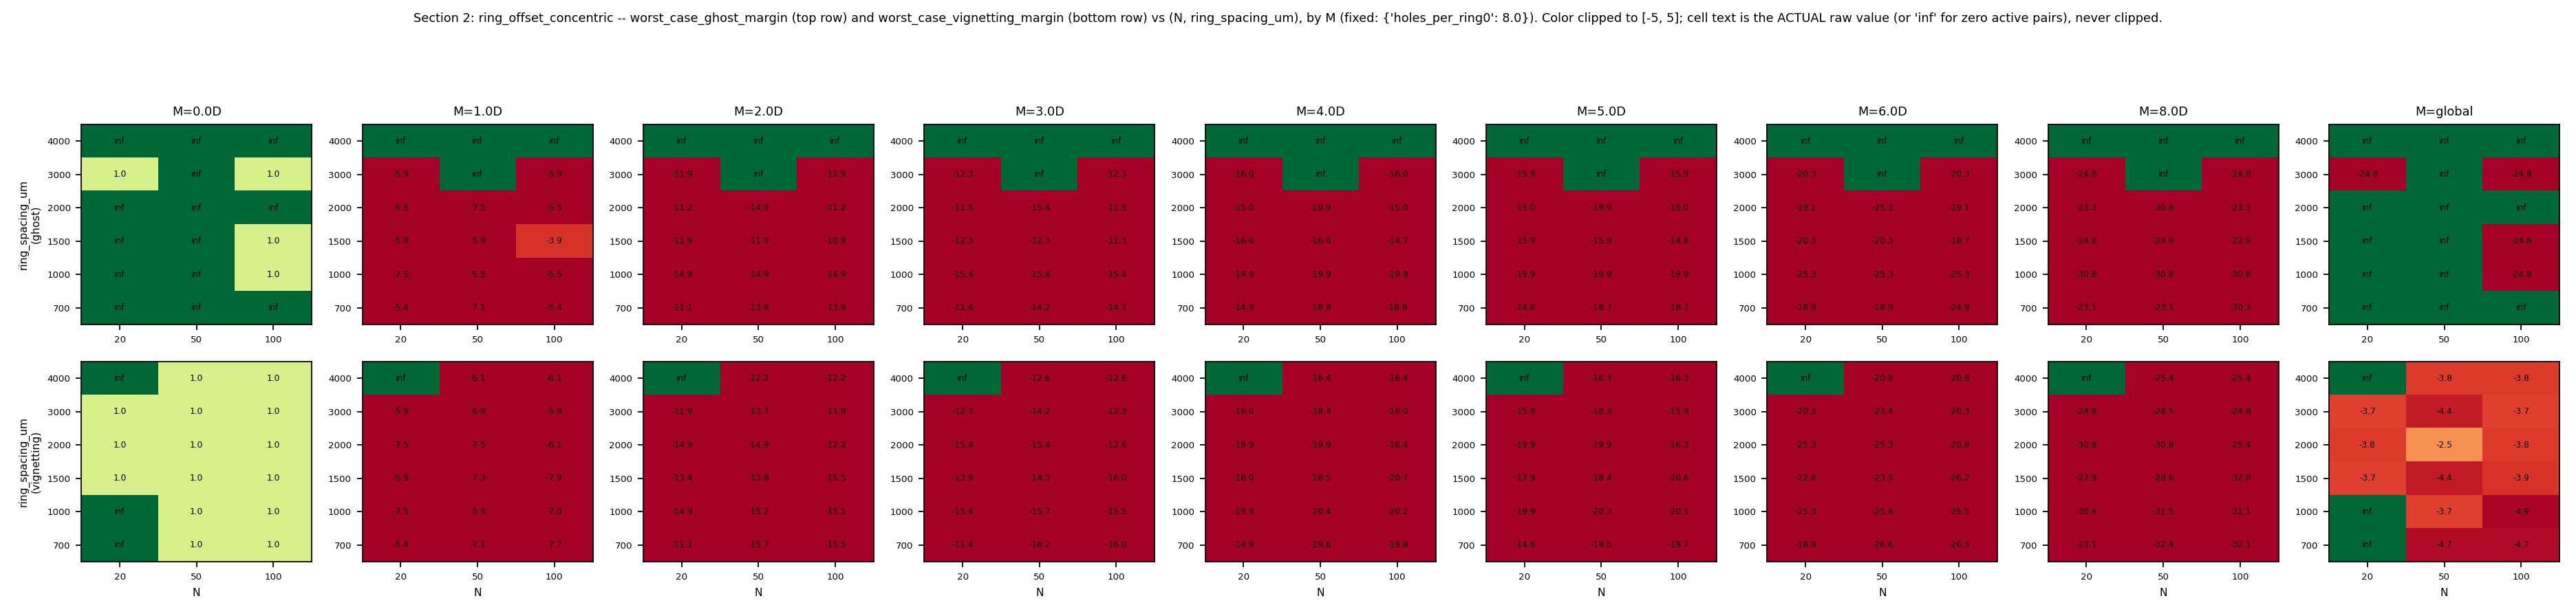
\includegraphics[width=\textwidth]{figs_exploration/section2_heatmap_ring_offset_concentric.png}
\caption{ring\_offset\_concentric: worst\_case\_ghost\_margin (top row) and worst\_case\_vignetting\_margin (bottom row) vs.\ $(N, \text{ring\_spacing\_um})$, by $M$. holes\_per\_ring0=8.0 held fixed at its own median tested value; axes: $N \in \{20,50,100\}$.}
\end{figure}
\begin{figure}[h!]
\centering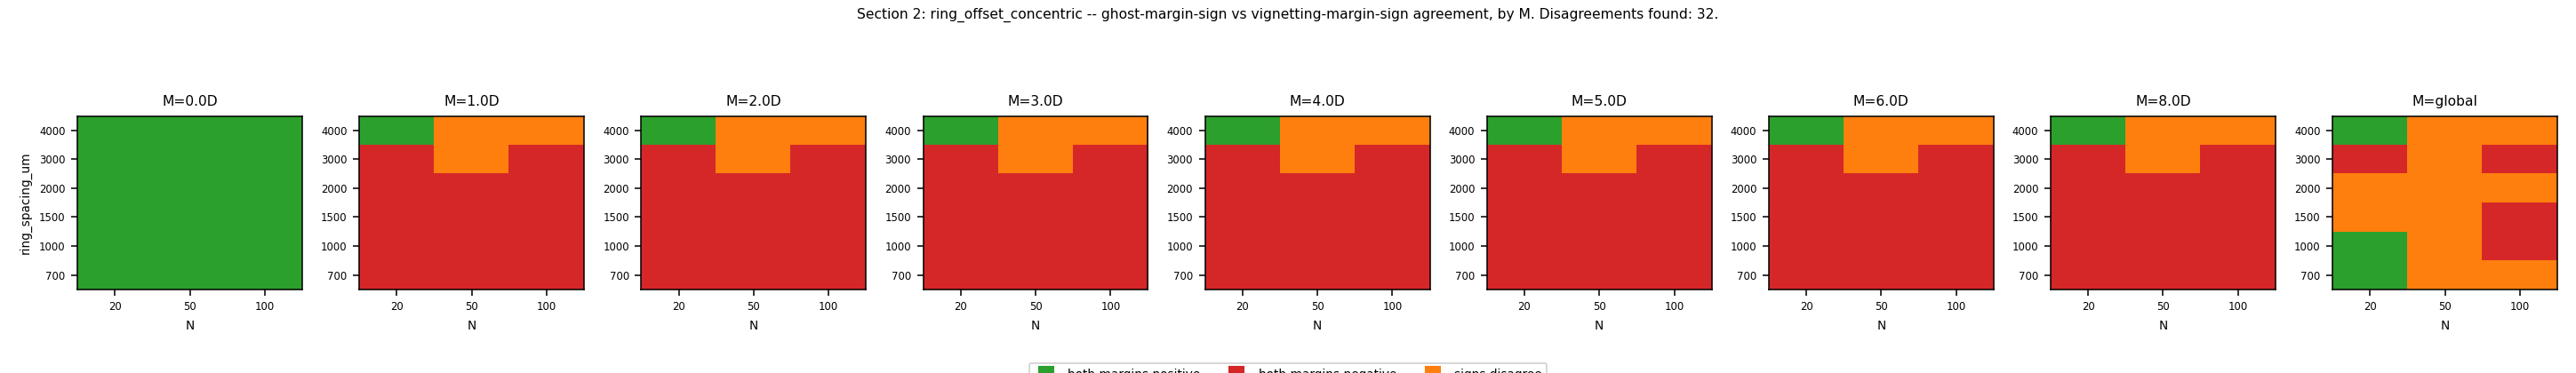
\includegraphics[width=\textwidth]{figs_exploration/section2_signagreement_ring_offset_concentric.png}
\caption{ring\_offset\_concentric: ghost-margin-sign vs.\ vignetting-margin-sign agreement, by $M$ (see the figure's own title for the exact disagreement count).}
\end{figure}
\clearpage
\begin{figure}[h!]
\centering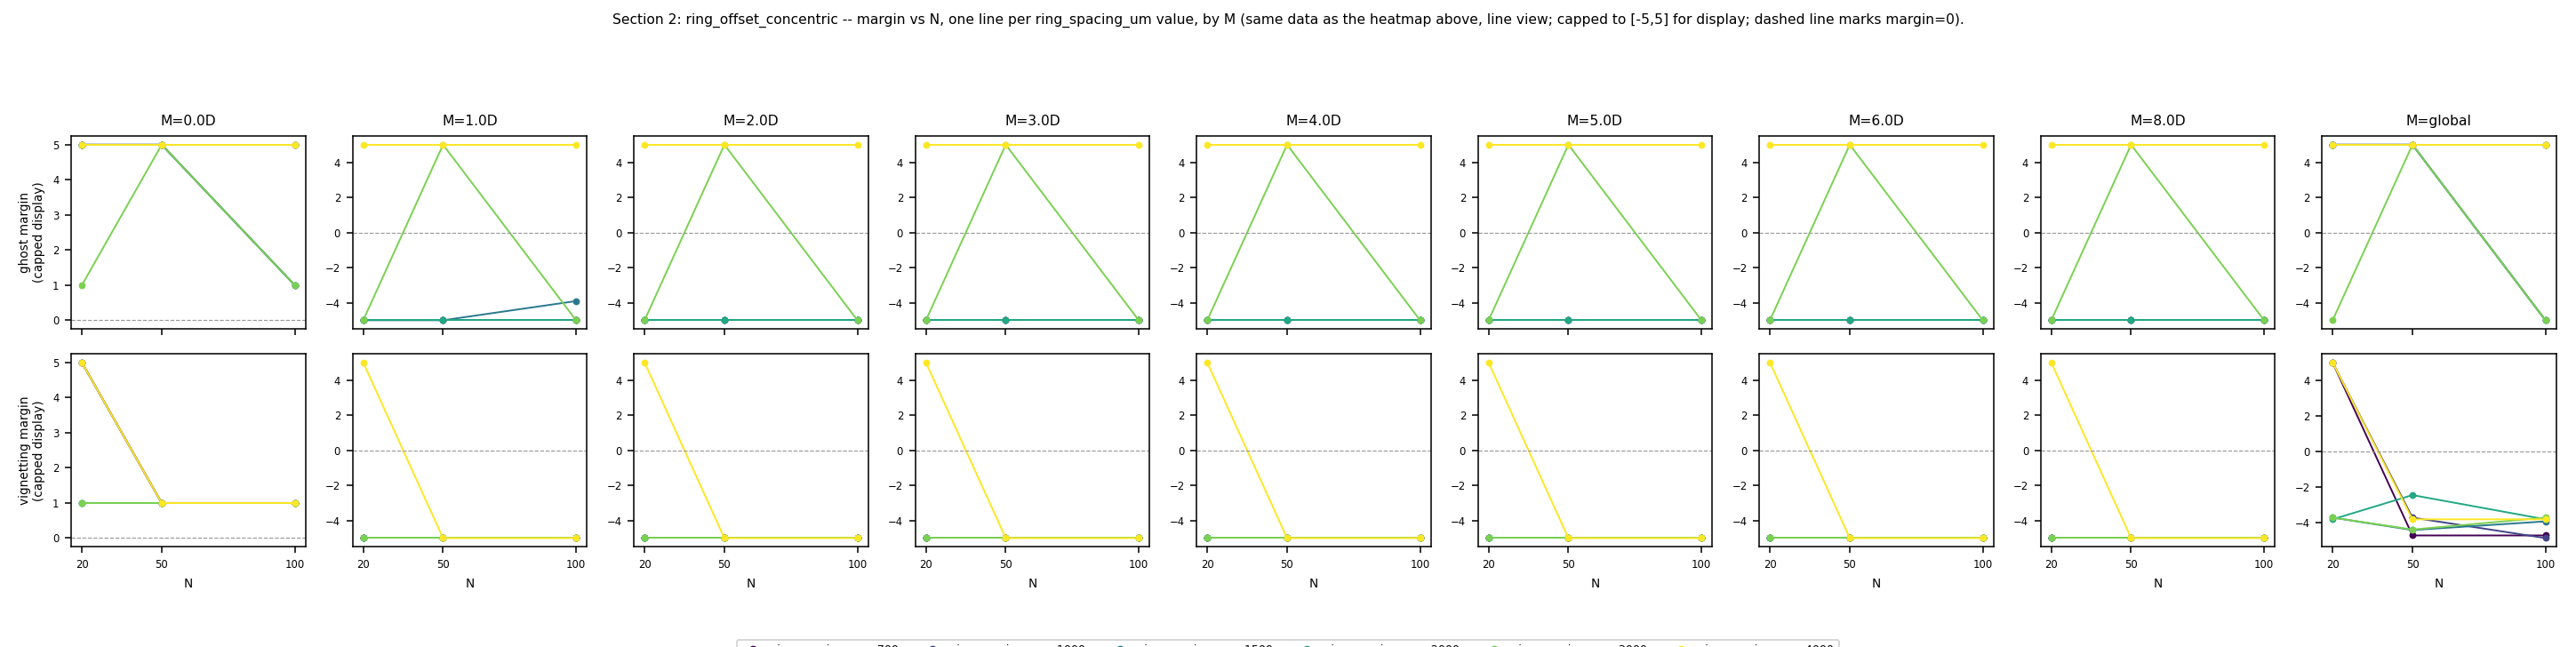
\includegraphics[width=\textwidth]{figs_exploration/section2_lineplot_ring_offset_concentric.png}
\caption{ring\_offset\_concentric: same margin data as the heatmap above, shown as line plots (margin vs.\ $N$, one line per ring\_spacing\_um value) -- a complementary graphical view for reading trends across $N$ directly.}
\end{figure}
\clearpage
\subsection*{ring\_offset\_concentric: raw number list}
\begin{longtable}{rrrrr}
\caption{ring\_offset\_concentric: raw worst\_case\_ghost\_margin and worst\_case\_vignetting\_margin values behind the heatmap and line plot above -- one row per tested $(N, ring\_spacing\_um, M)$ point. `inf' = zero active hole pairs under the pupil at that point (structurally safe, undisplayable on a linear scale).} \\
\toprule
N & ring\_spacing\_um & M & ghost\_margin & vignetting\_margin \\
\midrule
\endfirsthead
\toprule
N & ring\_spacing\_um & M & ghost\_margin & vignetting\_margin \\
\midrule
\endhead
\midrule
\multicolumn{5}{r}{\itshape continued on next page} \\
\endfoot
\bottomrule
\endlastfoot
20 & 700 & 0D & inf & inf \\
20 & 700 & 1D & -5.352 & -5.352 \\
20 & 700 & 2D & -11.052 & -11.052 \\
20 & 700 & 3D & -11.408 & -11.408 \\
20 & 700 & 4D & -14.870 & -14.870 \\
20 & 700 & 5D & -14.802 & -14.802 \\
20 & 700 & 6D & -18.904 & -18.904 \\
20 & 700 & 8D & -23.100 & -23.100 \\
20 & 700 & global & inf & inf \\
50 & 700 & 0D & inf & 1.000 \\
50 & 700 & 1D & -7.079 & -7.079 \\
50 & 700 & 2D & -13.787 & -15.702 \\
50 & 700 & 3D & -14.225 & -16.196 \\
50 & 700 & 4D & -18.796 & -19.615 \\
50 & 700 & 5D & -18.712 & -19.528 \\
50 & 700 & 6D & -18.904 & -26.583 \\
50 & 700 & 8D & -23.100 & -32.399 \\
50 & 700 & global & inf & -4.733 \\
100 & 700 & 0D & inf & 1.000 \\
100 & 700 & 1D & -5.352 & -7.703 \\
100 & 700 & 2D & -13.787 & -15.542 \\
100 & 700 & 3D & -14.225 & -16.031 \\
100 & 700 & 4D & -18.796 & -19.779 \\
100 & 700 & 5D & -18.712 & -19.691 \\
100 & 700 & 6D & -24.856 & -26.319 \\
100 & 700 & 8D & -30.307 & -32.079 \\
100 & 700 & global & inf & -4.733 \\
20 & 1000 & 0D & inf & inf \\
20 & 1000 & 1D & -7.548 & -7.548 \\
20 & 1000 & 2D & -14.907 & -14.907 \\
20 & 1000 & 3D & -15.377 & -15.377 \\
20 & 1000 & 4D & -19.945 & -19.945 \\
20 & 1000 & 5D & -19.857 & -19.857 \\
20 & 1000 & 6D & -25.270 & -25.270 \\
20 & 1000 & 8D & -30.808 & -30.808 \\
20 & 1000 & global & inf & inf \\
50 & 1000 & 0D & inf & 1.000 \\
50 & 1000 & 1D & -5.542 & -5.939 \\
50 & 1000 & 2D & -14.907 & -15.244 \\
50 & 1000 & 3D & -15.377 & -15.725 \\
50 & 1000 & 4D & -19.945 & -20.390 \\
50 & 1000 & 5D & -19.857 & -20.299 \\
50 & 1000 & 6D & -25.270 & -25.827 \\
50 & 1000 & 8D & -30.808 & -31.483 \\
50 & 1000 & global & inf & -3.729 \\
100 & 1000 & 0D & 1.000 & 1.000 \\
100 & 1000 & 1D & -5.542 & -6.995 \\
100 & 1000 & 2D & -14.907 & -15.070 \\
100 & 1000 & 3D & -15.377 & -15.545 \\
100 & 1000 & 4D & -19.945 & -20.160 \\
100 & 1000 & 5D & -19.857 & -20.071 \\
100 & 1000 & 6D & -25.270 & -25.539 \\
100 & 1000 & 8D & -30.808 & -31.135 \\
100 & 1000 & global & -24.822 & -4.882 \\
20 & 1500 & 0D & inf & 1.000 \\
20 & 1500 & 1D & -5.939 & -5.939 \\
20 & 1500 & 2D & -11.913 & -13.437 \\
20 & 1500 & 3D & -12.295 & -13.864 \\
20 & 1500 & 4D & -16.003 & -18.010 \\
20 & 1500 & 5D & -15.931 & -17.930 \\
20 & 1500 & 6D & -20.326 & -22.843 \\
20 & 1500 & 8D & -24.822 & -27.870 \\
20 & 1500 & global & inf & -3.729 \\
50 & 1500 & 0D & inf & 1.000 \\
50 & 1500 & 1D & -5.939 & -7.325 \\
50 & 1500 & 2D & -11.913 & -13.825 \\
50 & 1500 & 3D & -12.295 & -14.263 \\
50 & 1500 & 4D & -16.003 & -18.521 \\
50 & 1500 & 5D & -15.931 & -18.438 \\
50 & 1500 & 6D & -20.326 & -23.483 \\
50 & 1500 & 8D & -24.822 & -28.645 \\
50 & 1500 & global & inf & -4.429 \\
100 & 1500 & 0D & 1.000 & 1.000 \\
100 & 1500 & 1D & -3.907 & -7.867 \\
100 & 1500 & 2D & -10.930 & -15.500 \\
100 & 1500 & 3D & -11.283 & -15.988 \\
100 & 1500 & 4D & -14.709 & -20.726 \\
100 & 1500 & 5D & -14.642 & -20.634 \\
100 & 1500 & 6D & -18.702 & -26.249 \\
100 & 1500 & 8D & -22.856 & -31.994 \\
100 & 1500 & global & -24.822 & -3.942 \\
20 & 2000 & 0D & inf & 1.000 \\
20 & 2000 & 1D & -5.542 & -7.548 \\
20 & 2000 & 2D & -11.175 & -14.907 \\
20 & 2000 & 3D & -11.534 & -15.377 \\
20 & 2000 & 4D & -15.031 & -19.945 \\
20 & 2000 & 5D & -14.963 & -19.857 \\
20 & 2000 & 6D & -19.106 & -25.270 \\
20 & 2000 & 8D & -23.345 & -30.808 \\
20 & 2000 & global & inf & -3.825 \\
50 & 2000 & 0D & inf & 1.000 \\
50 & 2000 & 1D & -7.548 & -7.548 \\
50 & 2000 & 2D & -14.907 & -14.907 \\
50 & 2000 & 3D & -15.377 & -15.377 \\
50 & 2000 & 4D & -19.945 & -19.945 \\
50 & 2000 & 5D & -19.857 & -19.857 \\
50 & 2000 & 6D & -25.270 & -25.270 \\
50 & 2000 & 8D & -30.808 & -30.808 \\
50 & 2000 & global & inf & -2.461 \\
100 & 2000 & 0D & inf & 1.000 \\
100 & 2000 & 1D & -5.542 & -6.081 \\
100 & 2000 & 2D & -11.175 & -12.178 \\
100 & 2000 & 3D & -11.534 & -12.567 \\
100 & 2000 & 4D & -15.031 & -16.352 \\
100 & 2000 & 5D & -14.963 & -16.278 \\
100 & 2000 & 6D & -19.106 & -20.763 \\
100 & 2000 & 8D & -23.345 & -25.351 \\
100 & 2000 & global & inf & -3.825 \\
20 & 3000 & 0D & 1.000 & 1.000 \\
20 & 3000 & 1D & -5.939 & -5.939 \\
20 & 3000 & 2D & -11.913 & -11.913 \\
20 & 3000 & 3D & -12.295 & -12.295 \\
20 & 3000 & 4D & -16.003 & -16.003 \\
20 & 3000 & 5D & -15.931 & -15.931 \\
20 & 3000 & 6D & -20.326 & -20.326 \\
20 & 3000 & 8D & -24.822 & -24.822 \\
20 & 3000 & global & -24.822 & -3.729 \\
50 & 3000 & 0D & inf & 1.000 \\
50 & 3000 & 1D & inf & -6.926 \\
50 & 3000 & 2D & inf & -13.748 \\
50 & 3000 & 3D & inf & -14.185 \\
50 & 3000 & 4D & inf & -18.420 \\
50 & 3000 & 5D & inf & -18.338 \\
50 & 3000 & 6D & inf & -23.357 \\
50 & 3000 & 8D & inf & -28.492 \\
50 & 3000 & global & inf & -4.401 \\
100 & 3000 & 0D & 1.000 & 1.000 \\
100 & 3000 & 1D & -5.939 & -5.939 \\
100 & 3000 & 2D & -11.913 & -11.913 \\
100 & 3000 & 3D & -12.295 & -12.295 \\
100 & 3000 & 4D & -16.003 & -16.003 \\
100 & 3000 & 5D & -15.931 & -15.931 \\
100 & 3000 & 6D & -20.326 & -20.326 \\
100 & 3000 & 8D & -24.822 & -24.822 \\
100 & 3000 & global & -24.822 & -3.729 \\
20 & 4000 & 0D & inf & inf \\
20 & 4000 & 1D & inf & inf \\
20 & 4000 & 2D & inf & inf \\
20 & 4000 & 3D & inf & inf \\
20 & 4000 & 4D & inf & inf \\
20 & 4000 & 5D & inf & inf \\
20 & 4000 & 6D & inf & inf \\
20 & 4000 & 8D & inf & inf \\
20 & 4000 & global & inf & inf \\
50 & 4000 & 0D & inf & 1.000 \\
50 & 4000 & 1D & inf & -6.081 \\
50 & 4000 & 2D & inf & -12.178 \\
50 & 4000 & 3D & inf & -12.567 \\
50 & 4000 & 4D & inf & -16.352 \\
50 & 4000 & 5D & inf & -16.278 \\
50 & 4000 & 6D & inf & -20.763 \\
50 & 4000 & 8D & inf & -25.351 \\
50 & 4000 & global & inf & -3.825 \\
100 & 4000 & 0D & inf & 1.000 \\
100 & 4000 & 1D & inf & -6.081 \\
100 & 4000 & 2D & inf & -12.178 \\
100 & 4000 & 3D & inf & -12.567 \\
100 & 4000 & 4D & inf & -16.352 \\
100 & 4000 & 5D & inf & -16.278 \\
100 & 4000 & 6D & inf & -20.763 \\
100 & 4000 & 8D & inf & -25.351 \\
100 & 4000 & global & inf & -3.825 \\
\end{longtable}

\clearpage

\section{square}
\begin{figure}[h!]
\centering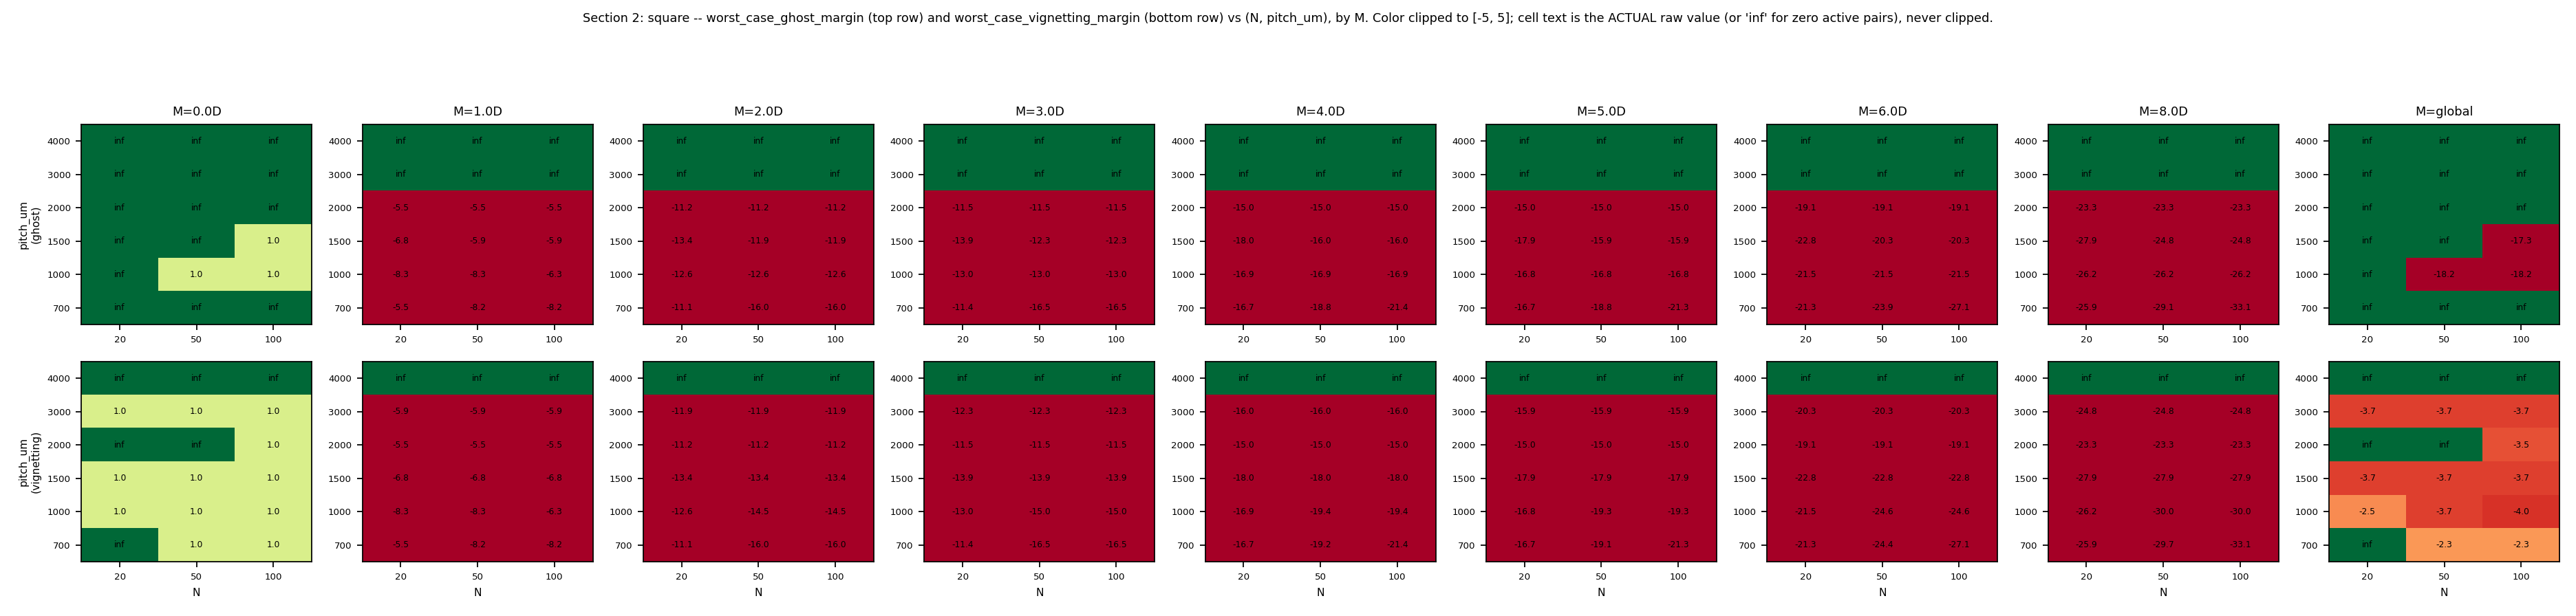
\includegraphics[width=\textwidth]{figs_exploration/section2_heatmap_square.png}
\caption{square: worst\_case\_ghost\_margin (top row) and worst\_case\_vignetting\_margin (bottom row) vs.\ $(N, \text{pitch\_um})$, by $M$. axes: $N \in \{20,50,100\}$.}
\end{figure}
\begin{figure}[h!]
\centering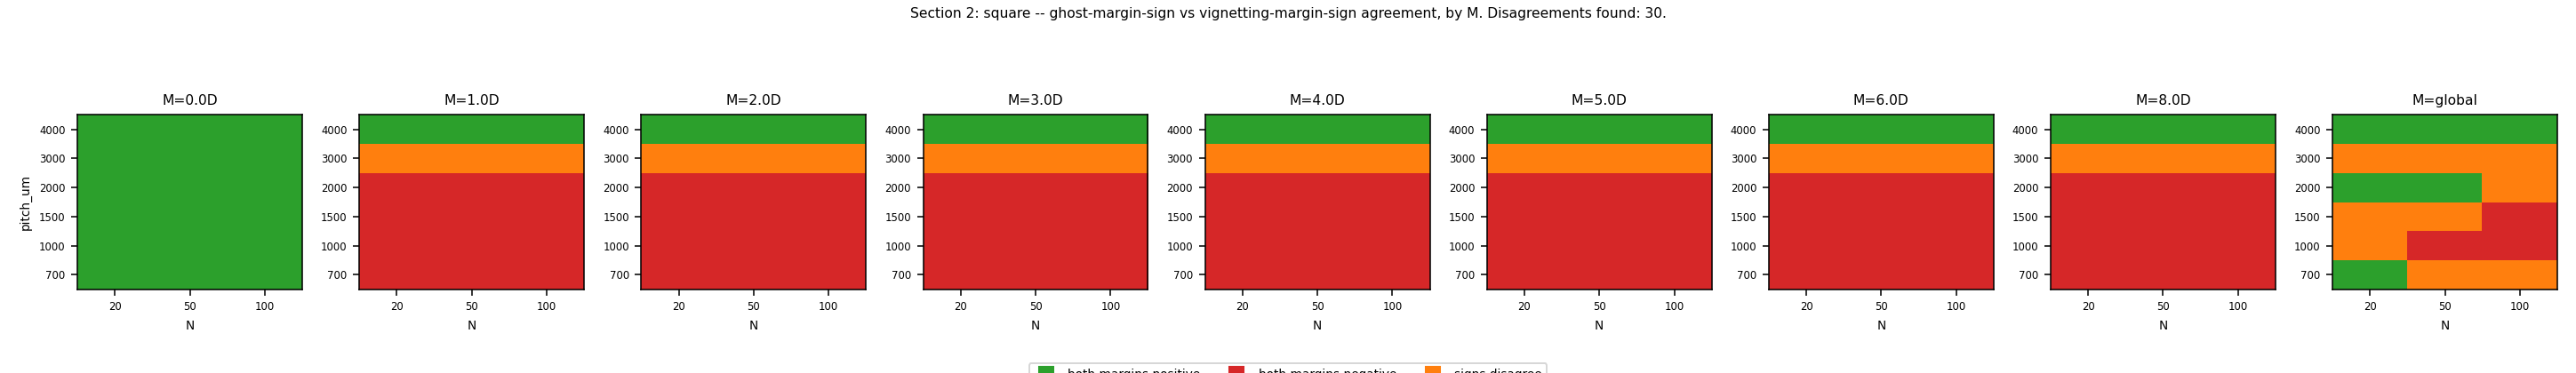
\includegraphics[width=\textwidth]{figs_exploration/section2_signagreement_square.png}
\caption{square: ghost-margin-sign vs.\ vignetting-margin-sign agreement, by $M$ (see the figure's own title for the exact disagreement count).}
\end{figure}
\clearpage
\begin{figure}[h!]
\centering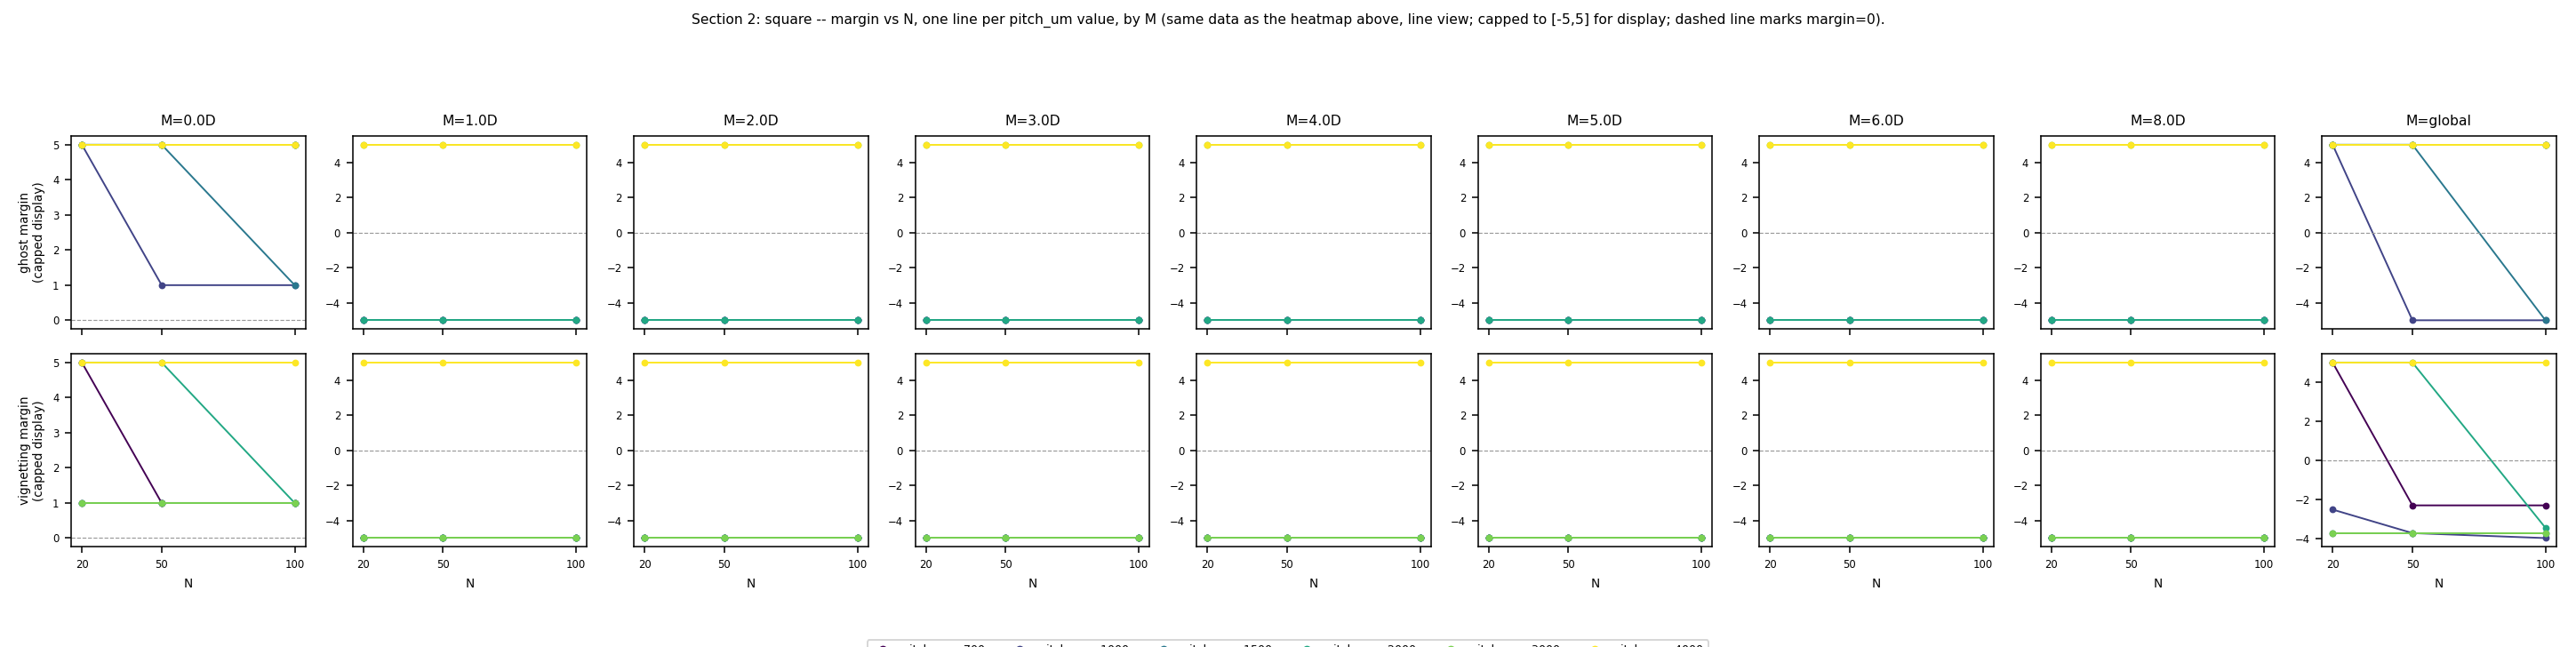
\includegraphics[width=\textwidth]{figs_exploration/section2_lineplot_square.png}
\caption{square: same margin data as the heatmap above, shown as line plots (margin vs.\ $N$, one line per pitch\_um value) -- a complementary graphical view for reading trends across $N$ directly.}
\end{figure}
\clearpage
\subsection*{square: raw number list}
\begin{longtable}{rrrrr}
\caption{square: raw worst\_case\_ghost\_margin and worst\_case\_vignetting\_margin values behind the heatmap and line plot above -- one row per tested $(N, pitch\_um, M)$ point. `inf' = zero active hole pairs under the pupil at that point (structurally safe, undisplayable on a linear scale).} \\
\toprule
N & pitch\_um & M & ghost\_margin & vignetting\_margin \\
\midrule
\endfirsthead
\toprule
N & pitch\_um & M & ghost\_margin & vignetting\_margin \\
\midrule
\endhead
\midrule
\multicolumn{5}{r}{\itshape continued on next page} \\
\endfoot
\bottomrule
\endlastfoot
20 & 700 & 0D & inf & inf \\
20 & 700 & 1D & -5.477 & -5.477 \\
20 & 700 & 2D & -11.052 & -11.052 \\
20 & 700 & 3D & -11.408 & -11.408 \\
20 & 700 & 4D & -16.743 & -16.743 \\
20 & 700 & 5D & -16.668 & -16.668 \\
20 & 700 & 6D & -21.253 & -21.253 \\
20 & 700 & 8D & -25.945 & -25.945 \\
20 & 700 & global & inf & inf \\
50 & 700 & 0D & inf & 1.000 \\
50 & 700 & 1D & -8.159 & -8.159 \\
50 & 700 & 2D & -16.044 & -16.044 \\
50 & 700 & 3D & -16.548 & -16.548 \\
50 & 700 & 4D & -18.837 & -19.230 \\
50 & 700 & 5D & -18.753 & -19.144 \\
50 & 700 & 6D & -23.880 & -24.373 \\
50 & 700 & 8D & -29.125 & -29.722 \\
50 & 700 & global & inf & -2.310 \\
100 & 700 & 0D & inf & 1.000 \\
100 & 700 & 1D & -8.159 & -8.159 \\
100 & 700 & 2D & -16.044 & -16.044 \\
100 & 700 & 3D & -16.548 & -16.548 \\
100 & 700 & 4D & -21.443 & -21.443 \\
100 & 700 & 5D & -21.348 & -21.348 \\
100 & 700 & 6D & -27.148 & -27.148 \\
100 & 700 & 8D & -33.083 & -33.083 \\
100 & 700 & global & inf & -2.310 \\
20 & 1000 & 0D & inf & 1.000 \\
20 & 1000 & 1D & -8.252 & -8.252 \\
20 & 1000 & 2D & -12.612 & -12.612 \\
20 & 1000 & 3D & -13.014 & -13.014 \\
20 & 1000 & 4D & -16.923 & -16.923 \\
20 & 1000 & 5D & -16.847 & -16.847 \\
20 & 1000 & 6D & -21.479 & -21.479 \\
20 & 1000 & 8D & -26.218 & -26.218 \\
20 & 1000 & global & inf & -2.524 \\
50 & 1000 & 0D & 1.000 & 1.000 \\
50 & 1000 & 1D & -8.252 & -8.252 \\
50 & 1000 & 2D & -12.612 & -14.520 \\
50 & 1000 & 3D & -13.014 & -14.978 \\
50 & 1000 & 4D & -16.923 & -19.435 \\
50 & 1000 & 5D & -16.847 & -19.349 \\
50 & 1000 & 6D & -21.479 & -24.630 \\
50 & 1000 & 8D & -26.218 & -30.034 \\
50 & 1000 & global & -18.246 & -3.729 \\
100 & 1000 & 0D & 1.000 & 1.000 \\
100 & 1000 & 1D & -6.315 & -6.315 \\
100 & 1000 & 2D & -12.612 & -14.520 \\
100 & 1000 & 3D & -13.014 & -14.978 \\
100 & 1000 & 4D & -16.923 & -19.435 \\
100 & 1000 & 5D & -16.847 & -19.349 \\
100 & 1000 & 6D & -21.479 & -24.630 \\
100 & 1000 & 8D & -26.218 & -30.034 \\
100 & 1000 & global & -18.246 & -3.984 \\
20 & 1500 & 0D & inf & 1.000 \\
20 & 1500 & 1D & -6.758 & -6.758 \\
20 & 1500 & 2D & -13.437 & -13.437 \\
20 & 1500 & 3D & -13.864 & -13.864 \\
20 & 1500 & 4D & -18.010 & -18.010 \\
20 & 1500 & 5D & -17.930 & -17.930 \\
20 & 1500 & 6D & -22.843 & -22.843 \\
20 & 1500 & 8D & -27.870 & -27.870 \\
20 & 1500 & global & inf & -3.729 \\
50 & 1500 & 0D & inf & 1.000 \\
50 & 1500 & 1D & -5.939 & -6.758 \\
50 & 1500 & 2D & -11.913 & -13.437 \\
50 & 1500 & 3D & -12.295 & -13.864 \\
50 & 1500 & 4D & -16.003 & -18.010 \\
50 & 1500 & 5D & -15.931 & -17.930 \\
50 & 1500 & 6D & -20.326 & -22.843 \\
50 & 1500 & 8D & -24.822 & -27.870 \\
50 & 1500 & global & inf & -3.729 \\
100 & 1500 & 0D & 1.000 & 1.000 \\
100 & 1500 & 1D & -5.939 & -6.758 \\
100 & 1500 & 2D & -11.913 & -13.437 \\
100 & 1500 & 3D & -12.295 & -13.864 \\
100 & 1500 & 4D & -16.003 & -18.010 \\
100 & 1500 & 5D & -15.931 & -17.930 \\
100 & 1500 & 6D & -20.326 & -22.843 \\
100 & 1500 & 8D & -24.822 & -27.870 \\
100 & 1500 & global & -17.259 & -3.729 \\
20 & 2000 & 0D & inf & inf \\
20 & 2000 & 1D & -5.542 & -5.542 \\
20 & 2000 & 2D & -11.175 & -11.175 \\
20 & 2000 & 3D & -11.534 & -11.534 \\
20 & 2000 & 4D & -15.031 & -15.031 \\
20 & 2000 & 5D & -14.963 & -14.963 \\
20 & 2000 & 6D & -19.106 & -19.106 \\
20 & 2000 & 8D & -23.345 & -23.345 \\
20 & 2000 & global & inf & inf \\
50 & 2000 & 0D & inf & inf \\
50 & 2000 & 1D & -5.542 & -5.542 \\
50 & 2000 & 2D & -11.175 & -11.175 \\
50 & 2000 & 3D & -11.534 & -11.534 \\
50 & 2000 & 4D & -15.031 & -15.031 \\
50 & 2000 & 5D & -14.963 & -14.963 \\
50 & 2000 & 6D & -19.106 & -19.106 \\
50 & 2000 & 8D & -23.345 & -23.345 \\
50 & 2000 & global & inf & inf \\
100 & 2000 & 0D & inf & 1.000 \\
100 & 2000 & 1D & -5.542 & -5.542 \\
100 & 2000 & 2D & -11.175 & -11.175 \\
100 & 2000 & 3D & -11.534 & -11.534 \\
100 & 2000 & 4D & -15.031 & -15.031 \\
100 & 2000 & 5D & -14.963 & -14.963 \\
100 & 2000 & 6D & -19.106 & -19.106 \\
100 & 2000 & 8D & -23.345 & -23.345 \\
100 & 2000 & global & inf & -3.458 \\
20 & 3000 & 0D & inf & 1.000 \\
20 & 3000 & 1D & inf & -5.939 \\
20 & 3000 & 2D & inf & -11.913 \\
20 & 3000 & 3D & inf & -12.295 \\
20 & 3000 & 4D & inf & -16.003 \\
20 & 3000 & 5D & inf & -15.931 \\
20 & 3000 & 6D & inf & -20.326 \\
20 & 3000 & 8D & inf & -24.822 \\
20 & 3000 & global & inf & -3.729 \\
50 & 3000 & 0D & inf & 1.000 \\
50 & 3000 & 1D & inf & -5.939 \\
50 & 3000 & 2D & inf & -11.913 \\
50 & 3000 & 3D & inf & -12.295 \\
50 & 3000 & 4D & inf & -16.003 \\
50 & 3000 & 5D & inf & -15.931 \\
50 & 3000 & 6D & inf & -20.326 \\
50 & 3000 & 8D & inf & -24.822 \\
50 & 3000 & global & inf & -3.729 \\
100 & 3000 & 0D & inf & 1.000 \\
100 & 3000 & 1D & inf & -5.939 \\
100 & 3000 & 2D & inf & -11.913 \\
100 & 3000 & 3D & inf & -12.295 \\
100 & 3000 & 4D & inf & -16.003 \\
100 & 3000 & 5D & inf & -15.931 \\
100 & 3000 & 6D & inf & -20.326 \\
100 & 3000 & 8D & inf & -24.822 \\
100 & 3000 & global & inf & -3.729 \\
20 & 4000 & 0D & inf & inf \\
20 & 4000 & 1D & inf & inf \\
20 & 4000 & 2D & inf & inf \\
20 & 4000 & 3D & inf & inf \\
20 & 4000 & 4D & inf & inf \\
20 & 4000 & 5D & inf & inf \\
20 & 4000 & 6D & inf & inf \\
20 & 4000 & 8D & inf & inf \\
20 & 4000 & global & inf & inf \\
50 & 4000 & 0D & inf & inf \\
50 & 4000 & 1D & inf & inf \\
50 & 4000 & 2D & inf & inf \\
50 & 4000 & 3D & inf & inf \\
50 & 4000 & 4D & inf & inf \\
50 & 4000 & 5D & inf & inf \\
50 & 4000 & 6D & inf & inf \\
50 & 4000 & 8D & inf & inf \\
50 & 4000 & global & inf & inf \\
100 & 4000 & 0D & inf & inf \\
100 & 4000 & 1D & inf & inf \\
100 & 4000 & 2D & inf & inf \\
100 & 4000 & 3D & inf & inf \\
100 & 4000 & 4D & inf & inf \\
100 & 4000 & 5D & inf & inf \\
100 & 4000 & 6D & inf & inf \\
100 & 4000 & 8D & inf & inf \\
100 & 4000 & global & inf & inf \\
\end{longtable}

\clearpage



%======================================================================
\chapter{Seed Variance (poisson\_disk, jittered\_lattice)}
\label{ch:seedvariance}
%======================================================================
For each $(N, \text{spacing})$ combination actually swept, the distribution of
\texttt{worst\_case\_ghost\_margin} across all 8 tested seeds, held at a single
representative $M=4$D (chosen so the spread shown is seed-driven only -- pooling every
$M$ into one violin was tried first and rejected, since cross-$M$ variation is far
larger than seed variation and would dominate the plot; see the figure-generation
script's own documented reasoning). A companion scatter shows seed-to-seed standard
deviation vs.\ the mean margin at each $(N, \text{spacing}, M)$ point (all $M$ shown here,
each point's own std computed strictly across seeds at that one $M$) -- no threshold is
drawn on it; that is a later step.

\begin{figure}[h!]
\centering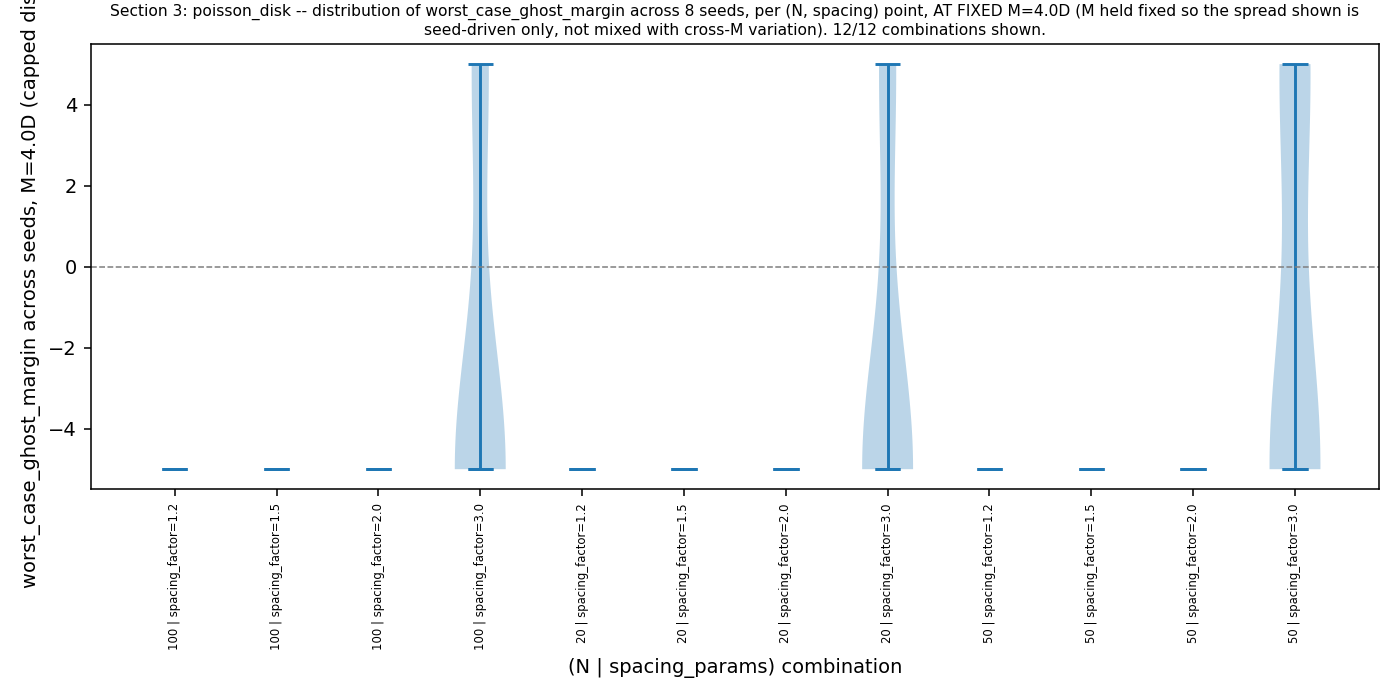
\includegraphics[width=\textwidth]{figs_exploration/section3_violin_poisson_disk.png}
\caption{poisson\_disk: margin distribution across 8 seeds, $M=4$D, per tested
$(N,\text{spacing})$ combination.}
\end{figure}
\begin{figure}[h!]
\centering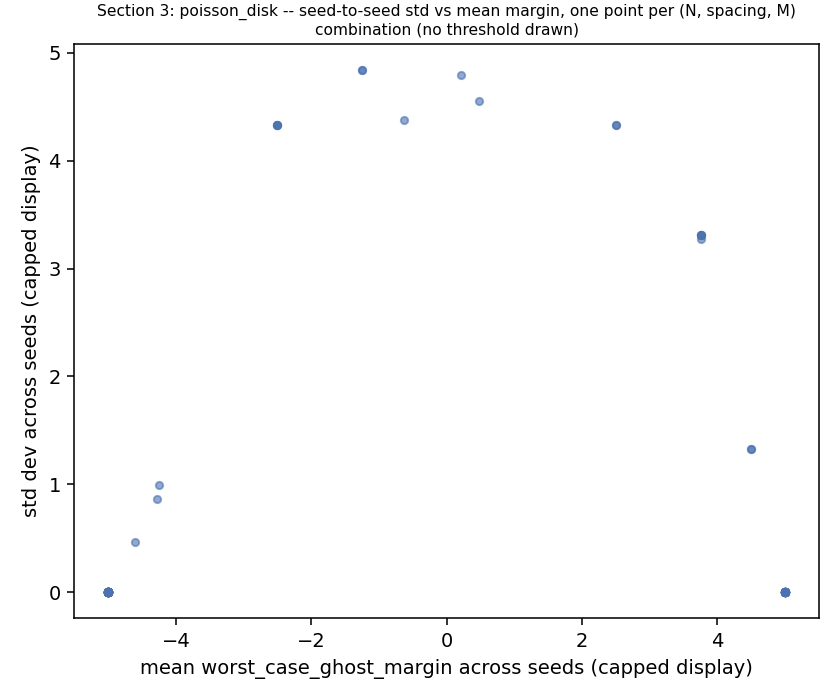
\includegraphics[width=0.6\textwidth]{figs_exploration/section3_std_vs_mean_poisson_disk.png}
\caption{poisson\_disk: seed-to-seed std vs.\ mean margin, one point per
$(N,\text{spacing},M)$.}
\end{figure}
\clearpage
\begin{figure}[h!]
\centering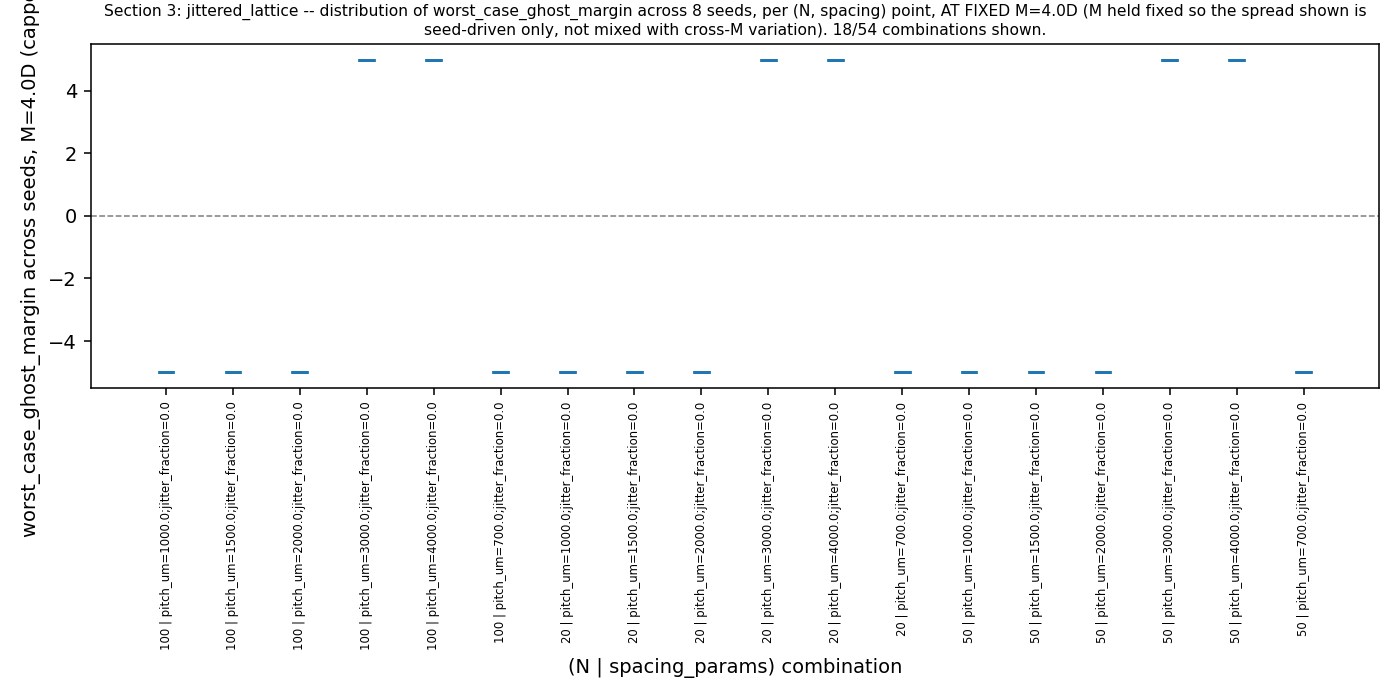
\includegraphics[width=\textwidth]{figs_exploration/section3_violin_jittered_lattice.png}
\caption{jittered\_lattice: margin distribution across 8 seeds, $M=4$D, per tested
$(N,\text{spacing})$ combination.}
\end{figure}
\begin{figure}[h!]
\centering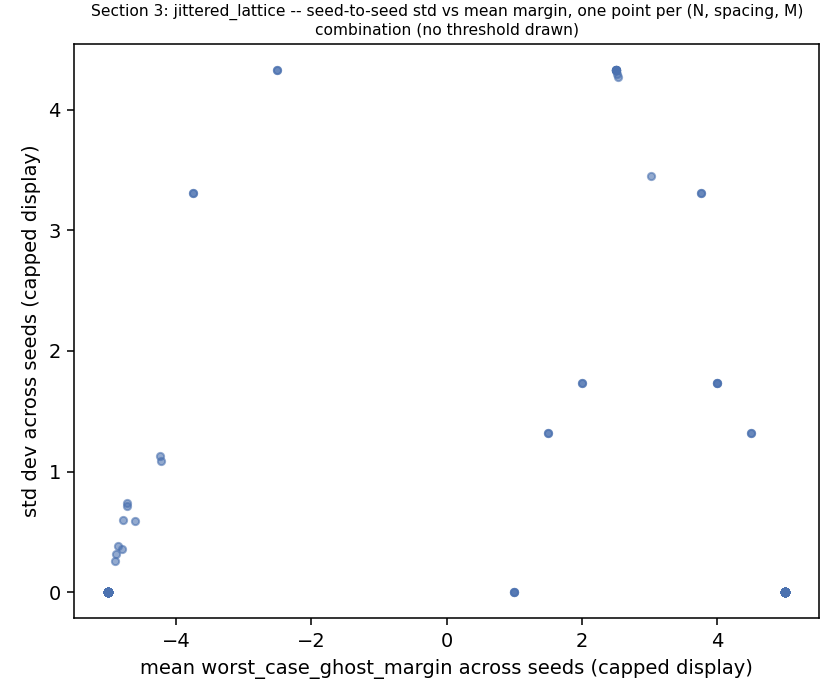
\includegraphics[width=0.6\textwidth]{figs_exploration/section3_std_vs_mean_jittered_lattice.png}
\caption{jittered\_lattice: seed-to-seed std vs.\ mean margin, one point per
$(N,\text{spacing},M)$.}
\end{figure}
\clearpage

%======================================================================
\chapter{Density vs. Safety}
%======================================================================
All structurally-safe candidates (\texttt{worst\_case\_ghost\_margin}$>0$ \textbf{and}
\texttt{worst\_case\_vignetting\_margin}$>0$, read directly from the CSV, not from any
gating script), across all 10 families, packing density on the $x$-axis vs.\
ghost margin on the $y$-axis, colored by family. Shown for $M=4$D and $M=\text{global}$
only (two representative cases, not the full $M$ grid, to keep this chapter to two
figures) -- $M=4$D as a representative mid-myopia single-$M$ case, $M=\text{global}$ as
the cross-$M$ worst-case scope.

\textbf{Density computation, stated explicitly}: packing density $=$
\texttt{N\_actual} / (area of the convex hull of the generated hole-center coordinates),
in holes per $\mu$m$^2$. The SAME convex-hull-area definition is applied uniformly to all
10 families (rather than a different closed-form cell-area formula per lattice type), so
density values are directly comparable on one axis; irregular families (spirals, rings,
stochastic patterns) have no closed-form cell area the way a lattice pitch does, so this
is the one measure that applies to all of them without a family-specific exception.
Coordinates are regenerated at each plotted point's own exact $(N, \text{spacing}[,
\text{seed}])$ to compute this -- not estimated.

\begin{figure}[h!]
\centering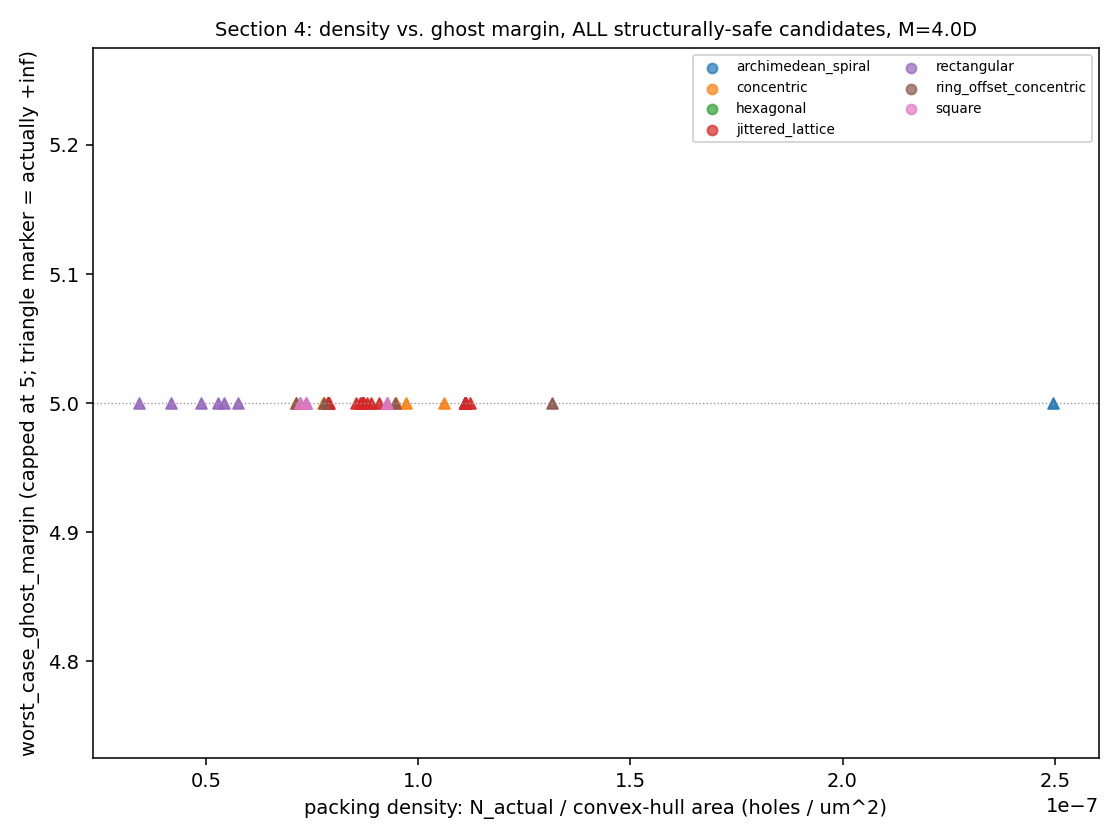
\includegraphics[width=0.85\textwidth]{figs_exploration/section4_density_vs_safety_M4.0.png}
\caption{Density vs.\ ghost margin, all structurally-safe candidates, $M=4$D.}
\end{figure}
\begin{figure}[h!]
\centering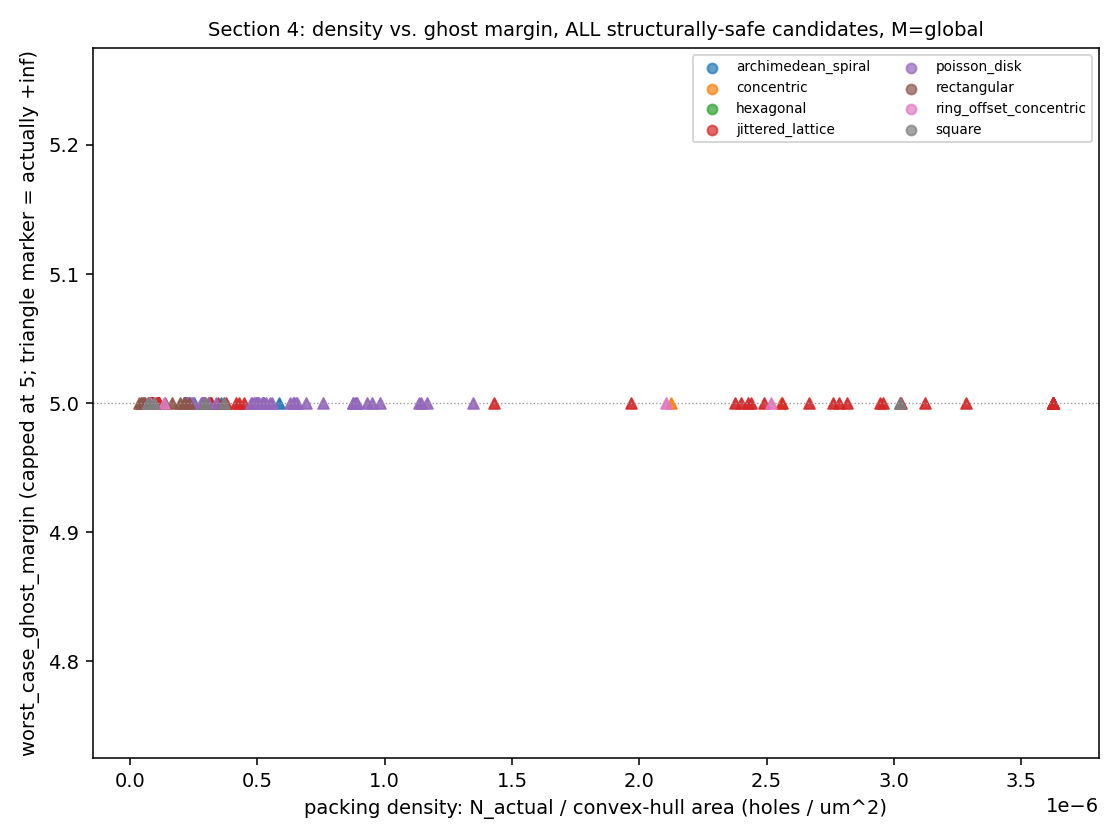
\includegraphics[width=0.85\textwidth]{figs_exploration/section4_density_vs_safety_Mglobal.png}
\caption{Density vs.\ ghost margin, all structurally-safe candidates, $M=\text{global}$.}
\end{figure}
\clearpage

%======================================================================
\chapter{Cross-Family Summary Table}
%======================================================================
One row per family, numbers read directly from \texttt{sweep\_results.csv} and
\texttt{family\_ranking.csv} by \texttt{generate\_exploration\_figures.py}
(\texttt{section5\_summary\_table()}), not computed by hand or typed into this document.
\texttt{best\_finite\_ghost\_margin} excludes $+\infty$ cells, reported separately as
\texttt{n\_inf\_margin\_rows}; seed-std columns apply only to the two stochastic families
and are computed across \emph{every} tested point (not only the ones that ended up
structurally safe overall -- restricting to safe-only was tried first and silently
excluded exactly the highest-variance points, since a point with a very negative
worst-case seed is, by definition, not in the safe set at all).

\begin{table}[h!]
\centering\small
\begin{tabular}{lrrrrrr}
\toprule
\textbf{family} & \textbf{N\_cand.} & \textbf{N\_safe} & \textbf{best\_finite} &
\textbf{N\_inf} & \textbf{mean\_std} & \textbf{max\_std} \\
\midrule
archimedean\_spiral & 15 & 26 & -3.337 & 66 & -- & -- \\
concentric & 36 & 78 & 1.000 & 102 & -- & -- \\
fibonacci\_spiral & 15 & 15 & 1.000 & 54 & -- & -- \\
golden\_angle & 15 & 15 & 1.000 & 54 & -- & -- \\
hexagonal & 18 & 43 & 1.000 & 76 & -- & -- \\
jittered\_lattice & 432 & 736 & 1.000 & 1740 & 0.182 & 4.330 \\
poisson\_disk & 96 & 180 & 1.000 & 302 & 0.656 & 4.841 \\
rectangular & 54 & 135 & 1.000 & 226 & -- & -- \\
ring\_offset\_concentric & 36 & 70 & 1.000 & 106 & -- & -- \\
square & 18 & 45 & 1.000 & 72 & -- & -- \\
\bottomrule

\end{tabular}
\caption{N\_cand. = number of distinct $(N,\text{spacing}[,\text{seed}])$ points tested;
N\_safe = rows with \texttt{structurally\_safe=True}; best\_finite =
largest \texttt{worst\_case\_ghost\_margin} excluding $+\infty$; N\_inf = count of
$+\infty$-margin rows; mean/max\_std = seed-to-seed std of \texttt{worst\_case\_ghost\_margin}
(poisson\_disk/jittered\_lattice only, ``--'' otherwise).}
\end{table}

\end{document}
